\documentclass[11pt]{article}

    \usepackage[breakable]{tcolorbox}
    \usepackage{parskip} % Stop auto-indenting (to mimic markdown behaviour)
    
    \usepackage{iftex}
    \ifPDFTeX
    	\usepackage[T1]{fontenc}
    	\usepackage{mathpazo}
    \else
    	\usepackage{fontspec}
    \fi

    % Basic figure setup, for now with no caption control since it's done
    % automatically by Pandoc (which extracts ![](path) syntax from Markdown).
    \usepackage{graphicx}
    % Maintain compatibility with old templates. Remove in nbconvert 6.0
    \let\Oldincludegraphics\includegraphics
    % Ensure that by default, figures have no caption (until we provide a
    % proper Figure object with a Caption API and a way to capture that
    % in the conversion process - todo).
    \usepackage{caption}
    \DeclareCaptionFormat{nocaption}{}
    \captionsetup{format=nocaption,aboveskip=0pt,belowskip=0pt}

    \usepackage{float}
    \floatplacement{figure}{H} % forces figures to be placed at the correct location
    \usepackage{xcolor} % Allow colors to be defined
    \usepackage{enumerate} % Needed for markdown enumerations to work
    \usepackage{geometry} % Used to adjust the document margins
    \usepackage{amsmath} % Equations
    \usepackage{amssymb} % Equations
    \usepackage{textcomp} % defines textquotesingle
    % Hack from http://tex.stackexchange.com/a/47451/13684:
    \AtBeginDocument{%
        \def\PYZsq{\textquotesingle}% Upright quotes in Pygmentized code
    }
    \usepackage{upquote} % Upright quotes for verbatim code
    \usepackage{eurosym} % defines \euro
    \usepackage[mathletters]{ucs} % Extended unicode (utf-8) support
    \usepackage{fancyvrb} % verbatim replacement that allows latex
    \usepackage{grffile} % extends the file name processing of package graphics 
                         % to support a larger range
    \makeatletter % fix for old versions of grffile with XeLaTeX
    \@ifpackagelater{grffile}{2019/11/01}
    {
      % Do nothing on new versions
    }
    {
      \def\Gread@@xetex#1{%
        \IfFileExists{"\Gin@base".bb}%
        {\Gread@eps{\Gin@base.bb}}%
        {\Gread@@xetex@aux#1}%
      }
    }
    \makeatother
    \usepackage[Export]{adjustbox} % Used to constrain images to a maximum size
    \adjustboxset{max size={0.9\linewidth}{0.9\paperheight}}

    % The hyperref package gives us a pdf with properly built
    % internal navigation ('pdf bookmarks' for the table of contents,
    % internal cross-reference links, web links for URLs, etc.)
    \usepackage{hyperref}
    % The default LaTeX title has an obnoxious amount of whitespace. By default,
    % titling removes some of it. It also provides customization options.
    \usepackage{titling}
    \usepackage{longtable} % longtable support required by pandoc >1.10
    \usepackage{booktabs}  % table support for pandoc > 1.12.2
    \usepackage[inline]{enumitem} % IRkernel/repr support (it uses the enumerate* environment)
    \usepackage[normalem]{ulem} % ulem is needed to support strikethroughs (\sout)
                                % normalem makes italics be italics, not underlines
    \usepackage{mathrsfs}
    

    
    % Colors for the hyperref package
    \definecolor{urlcolor}{rgb}{0,.145,.698}
    \definecolor{linkcolor}{rgb}{.71,0.21,0.01}
    \definecolor{citecolor}{rgb}{.12,.54,.11}

    % ANSI colors
    \definecolor{ansi-black}{HTML}{3E424D}
    \definecolor{ansi-black-intense}{HTML}{282C36}
    \definecolor{ansi-red}{HTML}{E75C58}
    \definecolor{ansi-red-intense}{HTML}{B22B31}
    \definecolor{ansi-green}{HTML}{00A250}
    \definecolor{ansi-green-intense}{HTML}{007427}
    \definecolor{ansi-yellow}{HTML}{DDB62B}
    \definecolor{ansi-yellow-intense}{HTML}{B27D12}
    \definecolor{ansi-blue}{HTML}{208FFB}
    \definecolor{ansi-blue-intense}{HTML}{0065CA}
    \definecolor{ansi-magenta}{HTML}{D160C4}
    \definecolor{ansi-magenta-intense}{HTML}{A03196}
    \definecolor{ansi-cyan}{HTML}{60C6C8}
    \definecolor{ansi-cyan-intense}{HTML}{258F8F}
    \definecolor{ansi-white}{HTML}{C5C1B4}
    \definecolor{ansi-white-intense}{HTML}{A1A6B2}
    \definecolor{ansi-default-inverse-fg}{HTML}{FFFFFF}
    \definecolor{ansi-default-inverse-bg}{HTML}{000000}

    % common color for the border for error outputs.
    \definecolor{outerrorbackground}{HTML}{FFDFDF}

    % commands and environments needed by pandoc snippets
    % extracted from the output of `pandoc -s`
    \providecommand{\tightlist}{%
      \setlength{\itemsep}{0pt}\setlength{\parskip}{0pt}}
    \DefineVerbatimEnvironment{Highlighting}{Verbatim}{commandchars=\\\{\}}
    % Add ',fontsize=\small' for more characters per line
    \newenvironment{Shaded}{}{}
    \newcommand{\KeywordTok}[1]{\textcolor[rgb]{0.00,0.44,0.13}{\textbf{{#1}}}}
    \newcommand{\DataTypeTok}[1]{\textcolor[rgb]{0.56,0.13,0.00}{{#1}}}
    \newcommand{\DecValTok}[1]{\textcolor[rgb]{0.25,0.63,0.44}{{#1}}}
    \newcommand{\BaseNTok}[1]{\textcolor[rgb]{0.25,0.63,0.44}{{#1}}}
    \newcommand{\FloatTok}[1]{\textcolor[rgb]{0.25,0.63,0.44}{{#1}}}
    \newcommand{\CharTok}[1]{\textcolor[rgb]{0.25,0.44,0.63}{{#1}}}
    \newcommand{\StringTok}[1]{\textcolor[rgb]{0.25,0.44,0.63}{{#1}}}
    \newcommand{\CommentTok}[1]{\textcolor[rgb]{0.38,0.63,0.69}{\textit{{#1}}}}
    \newcommand{\OtherTok}[1]{\textcolor[rgb]{0.00,0.44,0.13}{{#1}}}
    \newcommand{\AlertTok}[1]{\textcolor[rgb]{1.00,0.00,0.00}{\textbf{{#1}}}}
    \newcommand{\FunctionTok}[1]{\textcolor[rgb]{0.02,0.16,0.49}{{#1}}}
    \newcommand{\RegionMarkerTok}[1]{{#1}}
    \newcommand{\ErrorTok}[1]{\textcolor[rgb]{1.00,0.00,0.00}{\textbf{{#1}}}}
    \newcommand{\NormalTok}[1]{{#1}}
    
    % Additional commands for more recent versions of Pandoc
    \newcommand{\ConstantTok}[1]{\textcolor[rgb]{0.53,0.00,0.00}{{#1}}}
    \newcommand{\SpecialCharTok}[1]{\textcolor[rgb]{0.25,0.44,0.63}{{#1}}}
    \newcommand{\VerbatimStringTok}[1]{\textcolor[rgb]{0.25,0.44,0.63}{{#1}}}
    \newcommand{\SpecialStringTok}[1]{\textcolor[rgb]{0.73,0.40,0.53}{{#1}}}
    \newcommand{\ImportTok}[1]{{#1}}
    \newcommand{\DocumentationTok}[1]{\textcolor[rgb]{0.73,0.13,0.13}{\textit{{#1}}}}
    \newcommand{\AnnotationTok}[1]{\textcolor[rgb]{0.38,0.63,0.69}{\textbf{\textit{{#1}}}}}
    \newcommand{\CommentVarTok}[1]{\textcolor[rgb]{0.38,0.63,0.69}{\textbf{\textit{{#1}}}}}
    \newcommand{\VariableTok}[1]{\textcolor[rgb]{0.10,0.09,0.49}{{#1}}}
    \newcommand{\ControlFlowTok}[1]{\textcolor[rgb]{0.00,0.44,0.13}{\textbf{{#1}}}}
    \newcommand{\OperatorTok}[1]{\textcolor[rgb]{0.40,0.40,0.40}{{#1}}}
    \newcommand{\BuiltInTok}[1]{{#1}}
    \newcommand{\ExtensionTok}[1]{{#1}}
    \newcommand{\PreprocessorTok}[1]{\textcolor[rgb]{0.74,0.48,0.00}{{#1}}}
    \newcommand{\AttributeTok}[1]{\textcolor[rgb]{0.49,0.56,0.16}{{#1}}}
    \newcommand{\InformationTok}[1]{\textcolor[rgb]{0.38,0.63,0.69}{\textbf{\textit{{#1}}}}}
    \newcommand{\WarningTok}[1]{\textcolor[rgb]{0.38,0.63,0.69}{\textbf{\textit{{#1}}}}}
    
    
    % Define a nice break command that doesn't care if a line doesn't already
    % exist.
    \def\br{\hspace*{\fill} \\* }
    % Math Jax compatibility definitions
    \def\gt{>}
    \def\lt{<}
    \let\Oldtex\TeX
    \let\Oldlatex\LaTeX
    \renewcommand{\TeX}{\textrm{\Oldtex}}
    \renewcommand{\LaTeX}{\textrm{\Oldlatex}}
    % Document parameters
    % Document title
    \title{Simulating Rutherford Scattering}
    \author{Freddie Nunn}
    
    
    
    
% Pygments definitions
\makeatletter
\def\PY@reset{\let\PY@it=\relax \let\PY@bf=\relax%
    \let\PY@ul=\relax \let\PY@tc=\relax%
    \let\PY@bc=\relax \let\PY@ff=\relax}
\def\PY@tok#1{\csname PY@tok@#1\endcsname}
\def\PY@toks#1+{\ifx\relax#1\empty\else%
    \PY@tok{#1}\expandafter\PY@toks\fi}
\def\PY@do#1{\PY@bc{\PY@tc{\PY@ul{%
    \PY@it{\PY@bf{\PY@ff{#1}}}}}}}
\def\PY#1#2{\PY@reset\PY@toks#1+\relax+\PY@do{#2}}

\@namedef{PY@tok@w}{\def\PY@tc##1{\textcolor[rgb]{0.73,0.73,0.73}{##1}}}
\@namedef{PY@tok@c}{\let\PY@it=\textit\def\PY@tc##1{\textcolor[rgb]{0.25,0.50,0.50}{##1}}}
\@namedef{PY@tok@cp}{\def\PY@tc##1{\textcolor[rgb]{0.74,0.48,0.00}{##1}}}
\@namedef{PY@tok@k}{\let\PY@bf=\textbf\def\PY@tc##1{\textcolor[rgb]{0.00,0.50,0.00}{##1}}}
\@namedef{PY@tok@kp}{\def\PY@tc##1{\textcolor[rgb]{0.00,0.50,0.00}{##1}}}
\@namedef{PY@tok@kt}{\def\PY@tc##1{\textcolor[rgb]{0.69,0.00,0.25}{##1}}}
\@namedef{PY@tok@o}{\def\PY@tc##1{\textcolor[rgb]{0.40,0.40,0.40}{##1}}}
\@namedef{PY@tok@ow}{\let\PY@bf=\textbf\def\PY@tc##1{\textcolor[rgb]{0.67,0.13,1.00}{##1}}}
\@namedef{PY@tok@nb}{\def\PY@tc##1{\textcolor[rgb]{0.00,0.50,0.00}{##1}}}
\@namedef{PY@tok@nf}{\def\PY@tc##1{\textcolor[rgb]{0.00,0.00,1.00}{##1}}}
\@namedef{PY@tok@nc}{\let\PY@bf=\textbf\def\PY@tc##1{\textcolor[rgb]{0.00,0.00,1.00}{##1}}}
\@namedef{PY@tok@nn}{\let\PY@bf=\textbf\def\PY@tc##1{\textcolor[rgb]{0.00,0.00,1.00}{##1}}}
\@namedef{PY@tok@ne}{\let\PY@bf=\textbf\def\PY@tc##1{\textcolor[rgb]{0.82,0.25,0.23}{##1}}}
\@namedef{PY@tok@nv}{\def\PY@tc##1{\textcolor[rgb]{0.10,0.09,0.49}{##1}}}
\@namedef{PY@tok@no}{\def\PY@tc##1{\textcolor[rgb]{0.53,0.00,0.00}{##1}}}
\@namedef{PY@tok@nl}{\def\PY@tc##1{\textcolor[rgb]{0.63,0.63,0.00}{##1}}}
\@namedef{PY@tok@ni}{\let\PY@bf=\textbf\def\PY@tc##1{\textcolor[rgb]{0.60,0.60,0.60}{##1}}}
\@namedef{PY@tok@na}{\def\PY@tc##1{\textcolor[rgb]{0.49,0.56,0.16}{##1}}}
\@namedef{PY@tok@nt}{\let\PY@bf=\textbf\def\PY@tc##1{\textcolor[rgb]{0.00,0.50,0.00}{##1}}}
\@namedef{PY@tok@nd}{\def\PY@tc##1{\textcolor[rgb]{0.67,0.13,1.00}{##1}}}
\@namedef{PY@tok@s}{\def\PY@tc##1{\textcolor[rgb]{0.73,0.13,0.13}{##1}}}
\@namedef{PY@tok@sd}{\let\PY@it=\textit\def\PY@tc##1{\textcolor[rgb]{0.73,0.13,0.13}{##1}}}
\@namedef{PY@tok@si}{\let\PY@bf=\textbf\def\PY@tc##1{\textcolor[rgb]{0.73,0.40,0.53}{##1}}}
\@namedef{PY@tok@se}{\let\PY@bf=\textbf\def\PY@tc##1{\textcolor[rgb]{0.73,0.40,0.13}{##1}}}
\@namedef{PY@tok@sr}{\def\PY@tc##1{\textcolor[rgb]{0.73,0.40,0.53}{##1}}}
\@namedef{PY@tok@ss}{\def\PY@tc##1{\textcolor[rgb]{0.10,0.09,0.49}{##1}}}
\@namedef{PY@tok@sx}{\def\PY@tc##1{\textcolor[rgb]{0.00,0.50,0.00}{##1}}}
\@namedef{PY@tok@m}{\def\PY@tc##1{\textcolor[rgb]{0.40,0.40,0.40}{##1}}}
\@namedef{PY@tok@gh}{\let\PY@bf=\textbf\def\PY@tc##1{\textcolor[rgb]{0.00,0.00,0.50}{##1}}}
\@namedef{PY@tok@gu}{\let\PY@bf=\textbf\def\PY@tc##1{\textcolor[rgb]{0.50,0.00,0.50}{##1}}}
\@namedef{PY@tok@gd}{\def\PY@tc##1{\textcolor[rgb]{0.63,0.00,0.00}{##1}}}
\@namedef{PY@tok@gi}{\def\PY@tc##1{\textcolor[rgb]{0.00,0.63,0.00}{##1}}}
\@namedef{PY@tok@gr}{\def\PY@tc##1{\textcolor[rgb]{1.00,0.00,0.00}{##1}}}
\@namedef{PY@tok@ge}{\let\PY@it=\textit}
\@namedef{PY@tok@gs}{\let\PY@bf=\textbf}
\@namedef{PY@tok@gp}{\let\PY@bf=\textbf\def\PY@tc##1{\textcolor[rgb]{0.00,0.00,0.50}{##1}}}
\@namedef{PY@tok@go}{\def\PY@tc##1{\textcolor[rgb]{0.53,0.53,0.53}{##1}}}
\@namedef{PY@tok@gt}{\def\PY@tc##1{\textcolor[rgb]{0.00,0.27,0.87}{##1}}}
\@namedef{PY@tok@err}{\def\PY@bc##1{{\setlength{\fboxsep}{\string -\fboxrule}\fcolorbox[rgb]{1.00,0.00,0.00}{1,1,1}{\strut ##1}}}}
\@namedef{PY@tok@kc}{\let\PY@bf=\textbf\def\PY@tc##1{\textcolor[rgb]{0.00,0.50,0.00}{##1}}}
\@namedef{PY@tok@kd}{\let\PY@bf=\textbf\def\PY@tc##1{\textcolor[rgb]{0.00,0.50,0.00}{##1}}}
\@namedef{PY@tok@kn}{\let\PY@bf=\textbf\def\PY@tc##1{\textcolor[rgb]{0.00,0.50,0.00}{##1}}}
\@namedef{PY@tok@kr}{\let\PY@bf=\textbf\def\PY@tc##1{\textcolor[rgb]{0.00,0.50,0.00}{##1}}}
\@namedef{PY@tok@bp}{\def\PY@tc##1{\textcolor[rgb]{0.00,0.50,0.00}{##1}}}
\@namedef{PY@tok@fm}{\def\PY@tc##1{\textcolor[rgb]{0.00,0.00,1.00}{##1}}}
\@namedef{PY@tok@vc}{\def\PY@tc##1{\textcolor[rgb]{0.10,0.09,0.49}{##1}}}
\@namedef{PY@tok@vg}{\def\PY@tc##1{\textcolor[rgb]{0.10,0.09,0.49}{##1}}}
\@namedef{PY@tok@vi}{\def\PY@tc##1{\textcolor[rgb]{0.10,0.09,0.49}{##1}}}
\@namedef{PY@tok@vm}{\def\PY@tc##1{\textcolor[rgb]{0.10,0.09,0.49}{##1}}}
\@namedef{PY@tok@sa}{\def\PY@tc##1{\textcolor[rgb]{0.73,0.13,0.13}{##1}}}
\@namedef{PY@tok@sb}{\def\PY@tc##1{\textcolor[rgb]{0.73,0.13,0.13}{##1}}}
\@namedef{PY@tok@sc}{\def\PY@tc##1{\textcolor[rgb]{0.73,0.13,0.13}{##1}}}
\@namedef{PY@tok@dl}{\def\PY@tc##1{\textcolor[rgb]{0.73,0.13,0.13}{##1}}}
\@namedef{PY@tok@s2}{\def\PY@tc##1{\textcolor[rgb]{0.73,0.13,0.13}{##1}}}
\@namedef{PY@tok@sh}{\def\PY@tc##1{\textcolor[rgb]{0.73,0.13,0.13}{##1}}}
\@namedef{PY@tok@s1}{\def\PY@tc##1{\textcolor[rgb]{0.73,0.13,0.13}{##1}}}
\@namedef{PY@tok@mb}{\def\PY@tc##1{\textcolor[rgb]{0.40,0.40,0.40}{##1}}}
\@namedef{PY@tok@mf}{\def\PY@tc##1{\textcolor[rgb]{0.40,0.40,0.40}{##1}}}
\@namedef{PY@tok@mh}{\def\PY@tc##1{\textcolor[rgb]{0.40,0.40,0.40}{##1}}}
\@namedef{PY@tok@mi}{\def\PY@tc##1{\textcolor[rgb]{0.40,0.40,0.40}{##1}}}
\@namedef{PY@tok@il}{\def\PY@tc##1{\textcolor[rgb]{0.40,0.40,0.40}{##1}}}
\@namedef{PY@tok@mo}{\def\PY@tc##1{\textcolor[rgb]{0.40,0.40,0.40}{##1}}}
\@namedef{PY@tok@ch}{\let\PY@it=\textit\def\PY@tc##1{\textcolor[rgb]{0.25,0.50,0.50}{##1}}}
\@namedef{PY@tok@cm}{\let\PY@it=\textit\def\PY@tc##1{\textcolor[rgb]{0.25,0.50,0.50}{##1}}}
\@namedef{PY@tok@cpf}{\let\PY@it=\textit\def\PY@tc##1{\textcolor[rgb]{0.25,0.50,0.50}{##1}}}
\@namedef{PY@tok@c1}{\let\PY@it=\textit\def\PY@tc##1{\textcolor[rgb]{0.25,0.50,0.50}{##1}}}
\@namedef{PY@tok@cs}{\let\PY@it=\textit\def\PY@tc##1{\textcolor[rgb]{0.25,0.50,0.50}{##1}}}

\def\PYZbs{\char`\\}
\def\PYZus{\char`\_}
\def\PYZob{\char`\{}
\def\PYZcb{\char`\}}
\def\PYZca{\char`\^}
\def\PYZam{\char`\&}
\def\PYZlt{\char`\<}
\def\PYZgt{\char`\>}
\def\PYZsh{\char`\#}
\def\PYZpc{\char`\%}
\def\PYZdl{\char`\$}
\def\PYZhy{\char`\-}
\def\PYZsq{\char`\'}
\def\PYZdq{\char`\"}
\def\PYZti{\char`\~}
% for compatibility with earlier versions
\def\PYZat{@}
\def\PYZlb{[}
\def\PYZrb{]}
\makeatother


    % For linebreaks inside Verbatim environment from package fancyvrb. 
    \makeatletter
        \newbox\Wrappedcontinuationbox 
        \newbox\Wrappedvisiblespacebox 
        \newcommand*\Wrappedvisiblespace {\textcolor{red}{\textvisiblespace}} 
        \newcommand*\Wrappedcontinuationsymbol {\textcolor{red}{\llap{\tiny$\m@th\hookrightarrow$}}} 
        \newcommand*\Wrappedcontinuationindent {3ex } 
        \newcommand*\Wrappedafterbreak {\kern\Wrappedcontinuationindent\copy\Wrappedcontinuationbox} 
        % Take advantage of the already applied Pygments mark-up to insert 
        % potential linebreaks for TeX processing. 
        %        {, <, #, %, $, ' and ": go to next line. 
        %        _, }, ^, &, >, - and ~: stay at end of broken line. 
        % Use of \textquotesingle for straight quote. 
        \newcommand*\Wrappedbreaksatspecials {% 
            \def\PYGZus{\discretionary{\char`\_}{\Wrappedafterbreak}{\char`\_}}% 
            \def\PYGZob{\discretionary{}{\Wrappedafterbreak\char`\{}{\char`\{}}% 
            \def\PYGZcb{\discretionary{\char`\}}{\Wrappedafterbreak}{\char`\}}}% 
            \def\PYGZca{\discretionary{\char`\^}{\Wrappedafterbreak}{\char`\^}}% 
            \def\PYGZam{\discretionary{\char`\&}{\Wrappedafterbreak}{\char`\&}}% 
            \def\PYGZlt{\discretionary{}{\Wrappedafterbreak\char`\<}{\char`\<}}% 
            \def\PYGZgt{\discretionary{\char`\>}{\Wrappedafterbreak}{\char`\>}}% 
            \def\PYGZsh{\discretionary{}{\Wrappedafterbreak\char`\#}{\char`\#}}% 
            \def\PYGZpc{\discretionary{}{\Wrappedafterbreak\char`\%}{\char`\%}}% 
            \def\PYGZdl{\discretionary{}{\Wrappedafterbreak\char`\$}{\char`\$}}% 
            \def\PYGZhy{\discretionary{\char`\-}{\Wrappedafterbreak}{\char`\-}}% 
            \def\PYGZsq{\discretionary{}{\Wrappedafterbreak\textquotesingle}{\textquotesingle}}% 
            \def\PYGZdq{\discretionary{}{\Wrappedafterbreak\char`\"}{\char`\"}}% 
            \def\PYGZti{\discretionary{\char`\~}{\Wrappedafterbreak}{\char`\~}}% 
        } 
        % Some characters . , ; ? ! / are not pygmentized. 
        % This macro makes them "active" and they will insert potential linebreaks 
        \newcommand*\Wrappedbreaksatpunct {% 
            \lccode`\~`\.\lowercase{\def~}{\discretionary{\hbox{\char`\.}}{\Wrappedafterbreak}{\hbox{\char`\.}}}% 
            \lccode`\~`\,\lowercase{\def~}{\discretionary{\hbox{\char`\,}}{\Wrappedafterbreak}{\hbox{\char`\,}}}% 
            \lccode`\~`\;\lowercase{\def~}{\discretionary{\hbox{\char`\;}}{\Wrappedafterbreak}{\hbox{\char`\;}}}% 
            \lccode`\~`\:\lowercase{\def~}{\discretionary{\hbox{\char`\:}}{\Wrappedafterbreak}{\hbox{\char`\:}}}% 
            \lccode`\~`\?\lowercase{\def~}{\discretionary{\hbox{\char`\?}}{\Wrappedafterbreak}{\hbox{\char`\?}}}% 
            \lccode`\~`\!\lowercase{\def~}{\discretionary{\hbox{\char`\!}}{\Wrappedafterbreak}{\hbox{\char`\!}}}% 
            \lccode`\~`\/\lowercase{\def~}{\discretionary{\hbox{\char`\/}}{\Wrappedafterbreak}{\hbox{\char`\/}}}% 
            \catcode`\.\active
            \catcode`\,\active 
            \catcode`\;\active
            \catcode`\:\active
            \catcode`\?\active
            \catcode`\!\active
            \catcode`\/\active 
            \lccode`\~`\~ 	
        }
    \makeatother

    \let\OriginalVerbatim=\Verbatim
    \makeatletter
    \renewcommand{\Verbatim}[1][1]{%
        %\parskip\z@skip
        \sbox\Wrappedcontinuationbox {\Wrappedcontinuationsymbol}%
        \sbox\Wrappedvisiblespacebox {\FV@SetupFont\Wrappedvisiblespace}%
        \def\FancyVerbFormatLine ##1{\hsize\linewidth
            \vtop{\raggedright\hyphenpenalty\z@\exhyphenpenalty\z@
                \doublehyphendemerits\z@\finalhyphendemerits\z@
                \strut ##1\strut}%
        }%
        % If the linebreak is at a space, the latter will be displayed as visible
        % space at end of first line, and a continuation symbol starts next line.
        % Stretch/shrink are however usually zero for typewriter font.
        \def\FV@Space {%
            \nobreak\hskip\z@ plus\fontdimen3\font minus\fontdimen4\font
            \discretionary{\copy\Wrappedvisiblespacebox}{\Wrappedafterbreak}
            {\kern\fontdimen2\font}%
        }%
        
        % Allow breaks at special characters using \PYG... macros.
        \Wrappedbreaksatspecials
        % Breaks at punctuation characters . , ; ? ! and / need catcode=\active 	
        \OriginalVerbatim[#1,codes*=\Wrappedbreaksatpunct]%
    }
    \makeatother

    % Exact colors from NB
    \definecolor{incolor}{HTML}{303F9F}
    \definecolor{outcolor}{HTML}{D84315}
    \definecolor{cellborder}{HTML}{CFCFCF}
    \definecolor{cellbackground}{HTML}{F7F7F7}
    
    % prompt
    \makeatletter
    \newcommand{\boxspacing}{\kern\kvtcb@left@rule\kern\kvtcb@boxsep}
    \makeatother
    \newcommand{\prompt}[4]{
        {\ttfamily\llap{{\color{#2}[#3]:\hspace{3pt}#4}}\vspace{-\baselineskip}}
    }
    

    
    % Prevent overflowing lines due to hard-to-break entities
    \sloppy 
    % Setup hyperref package
    \hypersetup{
      breaklinks=true,  % so long urls are correctly broken across lines
      colorlinks=true,
      urlcolor=urlcolor,
      linkcolor=linkcolor,
      citecolor=citecolor,
      }
    % Slightly bigger margins than the latex defaults
    
    \geometry{verbose,tmargin=1in,bmargin=1in,lmargin=1in,rmargin=1in}
    
    

\begin{document}

    	\begin{titlepage}
		\begin{center}
			\vspace*{1cm}
			
			\Huge
			\textbf{Simulating Rutherford Scattering}
			
			\vspace{0.5cm}
			\LARGE
			May 8, 2022
			
			\vspace{1.5cm}
			
			\textbf{Freddie Nunn}
			
			\vfill
			
			
			\vspace{0.8cm}
			
			\hypertarget{eton-college-computational-physics-prize-2022}{%
			\section*{Eton College Computational Physics Prize 2022}\label{eton-college-computational-physics-prize-2022}}
			
			
		\end{center}
	\end{titlepage}
    
	\pagebreak
	\begingroup
	\color{black}
	\tableofcontents
	\endgroup
	\pagebreak

 \hypertarget{introduction}{%
\section{Introduction}\label{introduction}}

\begin{center}\rule{0.5\linewidth}{0.5pt}\end{center}

\hypertarget{history-of-rutherford-scattering}{%
\subsection{History of Rutherford
Scattering}\label{history-of-rutherford-scattering}}

Rutherford Scattering is a phenomenon first explained by Ernest
Rutherford in 1911$^{\cite{rutherford_1911}}$; it describes the scattering of charged particles due
to the Coulomb Interaction (force between charged particles). The
phenomenon was first tested by Hans Geiger and Ernest Marsden in 1909$^{\cite{geiger_marsden_1913}}$
using the gold foil experiment, shown below:

\quad
\begin{figure}[!ht]
	\centering
	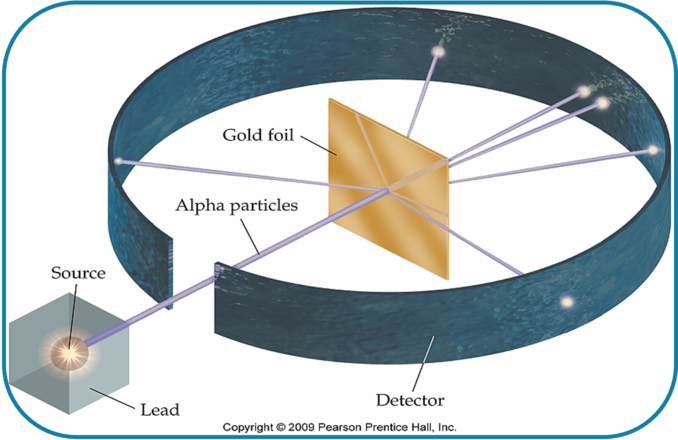
\includegraphics[width=0.8\textwidth]{../images/Hnet.com-image.png}
\end{figure}

The experiment consisted of bombarding a thin gold foil with alpha
particles from a radium source, and measuring the angle it comes out
with a fleorescent screen. At the time, the most widely accepted model
of an atom was Thomson's `plum pudding' model, which describes an atom
as a sperical region of positive charge with negative particles
scattered inside. According to this model, the particles should pass
through the atoms with very little deflections in their path, as there
is no large concentration of charge to deflect the particles. They found
most particles went through without much deflection, as expected, but a
few particles were deflected very large angles. This was not explained
until Rutherford published his paper in 1911 detailing the Rutherford
model of the atom, which consists of a small positive densely charged
area in the center of the atom called the nucleus, orbited by negative
particles. This explained the experiment's behaviour, as a small amount
of the alpha particles would get very close to the nucleus, exerting a
large force on the alpha particle, in turn causing a large deflection.
This model is very similar to the one used today, and was a big leap for
particle physics.

    \hypertarget{the-physics-of-rutherford-scattering}{%
\subsection{The Physics of Rutherford
Scattering}\label{the-physics-of-rutherford-scattering}}

Rutherford scattering is a direct consequence of Coulombs Law, which
describes the force between charged objects.
\[ {F = -\frac {1}{4\pi \epsilon_{0}}\frac {q_{1}q_{2}}{r^{2}}} \] Where
\(F\) is the force on the object in the direction of the other object,
\(\epsilon_{0}\) is the permutivity of a vacuum, \(q_{1}\) and \(q_{2}\)
are the charges of the objects, and \(r\) is the distance between them.
The main consequences of this in this context are: 1. The force between
the particles increases as they get closer 2. the direction of the force
on the alpha particle is directly away from the nucleus.

These 2 factors result in a behaviour where most of the particles'
trajectories are fairly unchanged, since they don't get close enough to
a nucleus for the force to be significant, but a few particles that get
close enough to the nucleus are pushed away, changing their trajectory
drastically. This change in trajectory is what Rutherford measured to
create his atom model, and is what I will be attempting to recreate.

    \hypertarget{model-overview}{%
\section{Model Overview}\label{model-overview}}

\begin{center}\rule{0.5\linewidth}{0.5pt}\end{center}

The aim of this model is to model Rutherford Scattering by simulating
the Gold Foil experiment that Geiger and Marsden performed. I will then
measure the distribution of scattering angles, and compare it to real
data to check its accuracy.

\hypertarget{factors-to-consider}{%
\subsection{Factors to Consider}\label{factors-to-consider}}

In order to create as accurate a model as possible, I will need to
consider all factors that could affect the scattering angle, and decide
whether to include them in my model or not.

\hypertarget{included-factors}{%
\subsubsection{Included Factors}\label{included-factors}}

\hypertarget{material-and-lattice-structure}{%
\subsubsection*{Material and Lattice
Structure}\label{material-and-lattice-structure}}
%
In the original experiment, they fired the alpha particles at a thin
leaf of gold lattice a few atoms thick. However, in Rutherford's paper
he repeated the experiment with multiple different materials, to verify
the scattering effect with different materials and investigate the
effect of different atom weights and sizes. In my model, varying the
material is much easier than Rutherford's experiment, and is just a
question of different numbers. My final model will also use a 3
Dimensional lattice to be as accurate as possible, but I will also model
a single atom and a 2 Dimensional lattice on the way, as they are easier
and allow me to more closely invesigate specific parts of the model.

\hypertarget{alpha-particle-velocity}{%
\subsubsection*{Alpha Particle Velocity}\label{alpha-particle-velocity}}
%
The velocity of the alpha particles directly affects the angle of
deflection, as the faster the particle is, the less time it spends close
to the nucleus and so it will be pushed less. In Rutherford's
experiments, he used a radium source to emit alpha particles with a
random distribution of velocities. However, I will use a constant
velocity for all of the alpha particles. While this means the results
may slightly differ from Rutherford's, it also means the results will be
more accurate, as each particle from the same position will be deflected
the same amount; A luxury unavailable to Rutherford at the time.

\hypertarget{effect-of-force-on-nucleus}{%
\subsubsection*{Effect of Force on
Nucleus}\label{effect-of-force-on-nucleus}}

The Coulomb Force acts on both particles involved, and so the nucleus
will also feel a repulsive force from the alpha particle. This creates a
small `recoil' in the nucleus, which can affect the deflection angle. I
will take the same approach as with the lattice structure, by
implementing it once I have a basic model completed.

\hypertarget{exluded-factors}{%
\subsubsection{Exluded Factors}\label{exluded-factors}}

\hypertarget{quantum-mechanics}{%
\subparagraph{Quantum Mechanics}\label{quantum-mechanics}}

I will be using the classical physics for this model. In reality, at
this microscopic level quantum physics starts to take over, which could
affect the results. However, these behaviours are very hard to
computationally model, so I will leave them out of this.

\hypertarget{relativistic-effects}{%
\subsubsection*{Relativistic Effects}\label{relativistic-effects}}

According to Einstein's Special Relativity, an object's mass is affected
by its velocity by a factor of
\(\frac {1}{\sqrt {1 - \frac {v^{2}}{c^{2}}}}\), where \(v\) is the
object's velocity and \(c\) is the speed of light in a vacuum. To decide
whether to include this in my model, I calculated the speed of an alpha
particle being emitted from a radium source. The alpha particles emitted
have \textasciitilde5.6 MeV of energy, and using
\(KE = \frac {1}{2}mv{2}\) and a mass of 4u, I found the speed to be
\textasciitilde{}\(1.6\times10^{7} m s^{-1}\). I then calculated the
relativistic mass using the factor stated earlier, and I got
\(6.7\times10^{-27}kg\). Finally, I calculated the \% change of mass
using the following formula: \[ \frac {m_{rel} - m}{m} \times 100\% \]
Where \(m\) is the standing mass and \(m_{rel}\) is the relativistic
mass, and got 0.15\% change. This shows that at these speeds, the change
in mass is neglegable, and I can safely assume the particles do not feel
these relativistic effects in my model, without significantly affecting
the results.

\hypertarget{charge-distribution-in-particles}{%
\subsubsection*{Charge Distribution in
Particles}\label{charge-distribution-in-particles}}

In my model, I will assume charge is distributed uniformly within the
particles. In reality, this is not true, as charge is contained in
discreet protons within the nucleus. However, Coulomb's Law only works
with point charges or uniformly distributed charge in a sphere, and so
this assumption must be made for the model to hold up. Once I have
completed the model, I may be able to depict this accurately by
considering the Coulomb force from each proton in a nucleus, increasing
the accuracy of the results.

    \hypertarget{model-breakdown}{%
\subsection{Model Breakdown}\label{model-breakdown}}

\hypertarget{parameters}{%
\subsubsection{Parameters}\label{parameters}}

The parameters for this model can be split into 3 main categories: alpha
particle, Nucleus, and simulation parameters.

\hypertarget{alpha-particle}{%
\subparagraph*{Alpha Particle}\label{alpha-particle}}

\begin{itemize}
\tightlist
\item
  \$ Q\_\{1\} \$: Charge of the particle
\item
  \(m_{\alpha}\): Mass of the particle
\item
  \(u\): Initial speed
\end{itemize}

The mass and charge of the particle will be based off the actual alpha
particle values. Initial speed will be chosen to follow Geiger and
Marsdon's original experiment as similarly as possible.

\hypertarget{nucleus}{%
\subparagraph*{Nucleus}\label{nucleus}}

\begin{itemize}
\tightlist
\item
  \(Q_{2}\): Charge of the nucleus
\item
  \(m_{n}\): Mass of the nucleus
\item
  \(r_{n}\): radius of the nucleus
\end{itemize}

The mass, charge and radius will be decided by the material being used.
This will be gold for most of the simulation to correlate with the
original experiments.

\hypertarget{simulation}{%
\subparagraph*{Simulation}\label{simulation}}

\begin{itemize}
\tightlist
\item
  \(a\): Activity of the source
\item
  \(r_{max}\): radius of source
\item
  \(n\): number of alpha particles
\item
  \(l\): Length of lattice
\item
  \(t\): thickness
\item
  \(d\): Distance from source to lattice
\end{itemize}

the activity decides the chance an alpha particle is created and will be
based off the radium source used in the original experiment. The radius
of the source determines the size of the area from wherer the alpha
particles are emitted. The number of alpha particles is the total number
emitted, and so determines how long the simulation will take and how
accurate the results will be. The length and thickness of the lattice
decide the size of the lattice that the alpha particles will be fired
into. The distance between source and lattice decides both how far away
alpha particles are when they are created, and the distance from the
lattice at which their scattering angle should be measured.

\hypertarget{the-simulation}{%
\subsubsection{The Simulation}\label{the-simulation}}

This describes the oultine of the simulation process.

\begin{enumerate}
\def\labelenumi{\arabic{enumi}.}
\tightlist
\item
  Initialize the atoms with positions according to the lattice shape and
  size, and values according the the material being used.
\item
  Choose whether to create an alpha particle or not randomly, according
  to the activity.

  \begin{itemize}
  \tightlist
  \item
    If an alpha particle is created, initialize it with a position
    randomly on a 2D plane representing the source.
  \end{itemize}
\item
  Calculate the net force on each alpha particle by combining the force
  from each nucleus.
\item
  Move forward a fixed timestep and change the alpha particles
  accordingly.
\item
  If an alpha particle is over \(d\) distance from the closest nucleus,
  measure its scattering angle, and delete the particle.
\item
  repeat steps 2-5 until \(n\) alpha particles have been created and
  deleted.
\end{enumerate}

    \hypertarget{algorithm-details}{%
\section{Algorithm Details}\label{algorithm-details}}

\begin{center}\rule{0.5\linewidth}{0.5pt}\end{center}

Here I will go over the details and mathematics involved with the
algorithms I will create.

    \hypertarget{distance-and-force}{%
\subsection{Distance and Force}\label{distance-and-force}}

The core algorithms in this model are calculating the distance and force
between particles. This forms the basis of how Rutherford Scattering
work.

Distance is calculated using the Euclidean Distance formula between 2
vectors A and B:
\[ r = \sqrt{(x_{A}-x_{B})^{2}+(y_{A}-y_{B})^{2}+(z_{A}-z_{B})^{2}} \]
and force can be calculated using Coulomb's Law.
\[ {|F| = \frac {Q_{A}Q_{B}}{4\pi \epsilon_{0}r^{2}}} \] This gives us
the magnitude of the force, but we then need to calculate the force
vector. Since both we know both particles will always be positive, the
direction of the force must be directly away from the other particle.
Therefore for a force on A, the direction is:
\[ \vec{BA} = \begin{pmatrix} x_{A}-x_{B} \\ y_{A}-y_{B}  \\  z_{A}-z_{B} \end{pmatrix} \]
We can now calculate the force vector. \[ F =  \lambda\times\vec{BA} \]
\[ |F| =  \lambda|\vec{BA}| \]
\[ F = \frac{|F|}{|\vec{BA}|}\times \vec{BA} \]

\hypertarget{net-force}{%
\subsubsection{Net Force}\label{net-force}}

Calculating the net force is as simple as adding up the forces from all
particles.
\[ \sum F = \sum_{i}\begin{pmatrix} x_{i} \\ y_{i}  \\  z_{i} \end{pmatrix} \]

    \hypertarget{update-position-and-velocity}{%
\subsection{Update Position and
Velocity}\label{update-position-and-velocity}}

I used a time integration method to update position and velocity in
discrete chunks of time. To do this, I used the Kinematic equations:
\[ v(t+\Delta t) = v(t) + a(t)\Delta t \]
\[ x(t+\Delta t) = x(t) + v(t+\Delta t)\Delta t \] Position and velocity
will both have starting values, and acceleration is calculated using
\(a=F/m\), where \(F\) is the net force on the particle. \(\Delta t\)
refers to the timestep, which will be calculated in a seperate
algorithm. I am using a semi-implicit method, where the velocity from
after the timestep is used to update the position; this is more accurate
than the explicit method of using the current velocity. You will notice
a fully implicit method where the acceleration from after the timstep is
used to update the velocity is not possible, as the position after the
timestep is needed for this, which we do not have. Therefore, the
equations to update velocity and position are as follows:
\[ v_{n+1} = v_{n} + \frac{\sum F}{m}\Delta t \]
\[ x_{n+1} = x_{n} + v_{n+1}\Delta t \]

    \hypertarget{calculate-timestep}{%
\subsubsection{Calculate Timestep}\label{calculate-timestep}}

The value of the timestep I use directly affects the efficiency and
accuracy of the program. Smaller timesteps give more accurate results,
but are slower. To improve efficiency and accuracy, I used a variable
timstep method, where the timstep is proportional to the smallest
distance from particle to nuclei. I also introduced a maximum and
minimum timestep to ensure accuracy and efficiency. Using trial and
error, I landed on \(10^{14}\) and \(10^{23}\) for the min and max
respectively, and \(10^{-9}\) for the proportional constant.
\[ \Delta t=max(min(d\times 10^{-9}, 10^{-14}), 10^{-23}) \]

    \hypertarget{calculate-angle}{%
\subsection{Calculate Angle}\label{calculate-angle}}

To calculate the total angle a particle has been deflected by, we can
use the equation for the dot product:
\[ A \cdot B = |A||B|cos(\theta) \] where A and B are vectors, and
\(\theta\) is the angle between them. since the direction of the
velocity vector of a particle represents the direction it is travelling,
the angle btween the initial velocity and the final velocity represents
the deflection angle. Thus, we can calculate the deflection angle as
follows:
\[ \theta = cos^{-1}(\frac{V_{0} \cdot V_{f}}{|V_{0}||V_{f}|}) \] Where
\(V_{0}\) is the initial velocity and \(V_{f}\) is the final velocity.

    \hypertarget{lattice-creation}{%
\subsection{Lattice creation}\label{lattice-creation}}

\hypertarget{single-nucleus}{%
\subsubsection{Single Nucleus}\label{single-nucleus}}

To create a single nucleus, a particle with 0 speed is initialized at
point \((0, 0, d)\).

\hypertarget{d-3d-lattice}{%
\subsubsection{2D \& 3D Lattice}\label{d-3d-lattice}}

The gold lattice is arranged in a face-centered cubic lattice; this is
where the lattice is made of multiple unit boxes stacked together, each
box having a particle at each corner and the centre of each face, as
shown.

\quad
\begin{figure}[!ht]
	\centering
	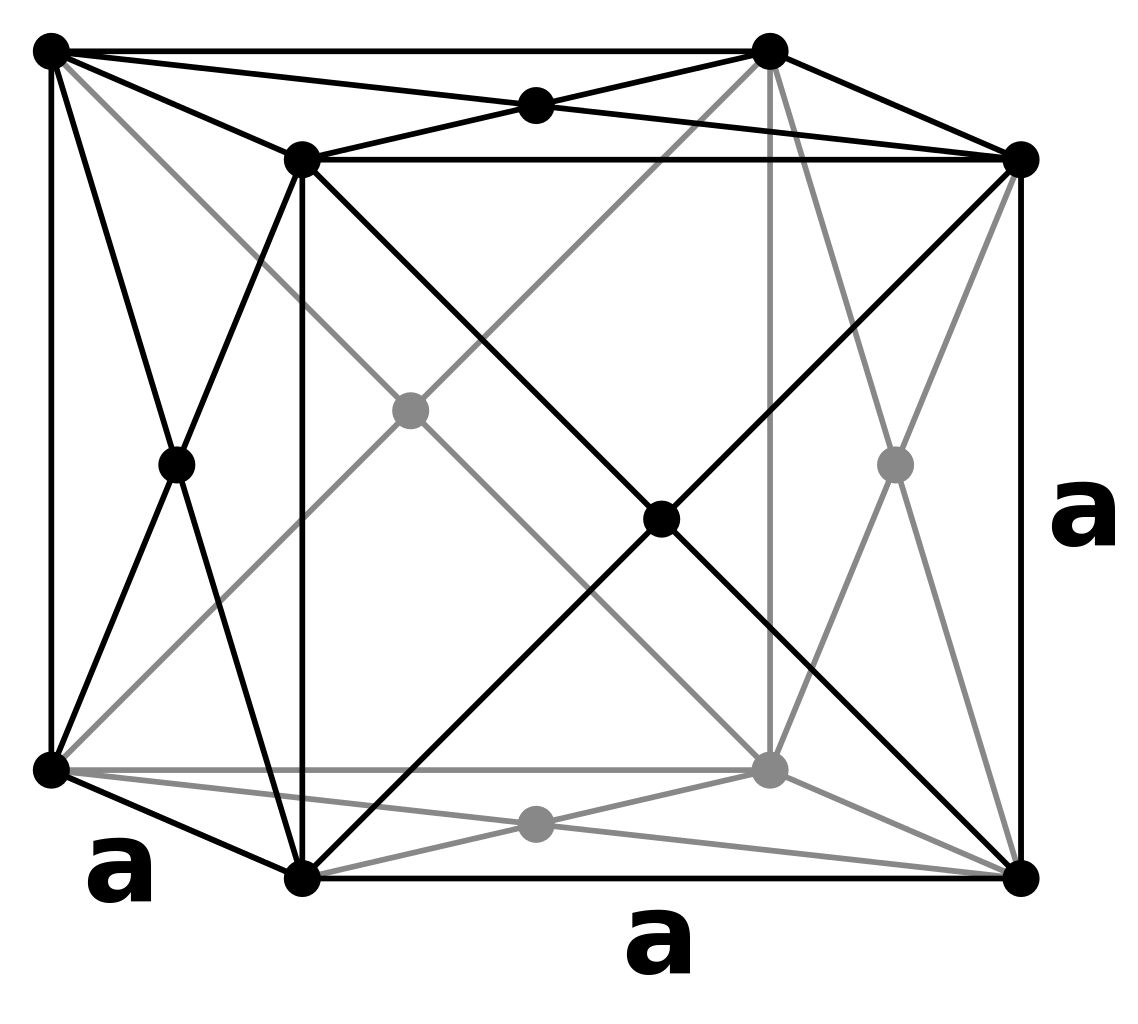
\includegraphics[width=0.4\textwidth]{../images/FaceCentredCubic.png}
\end{figure}

The length, \(a\), of the unit cube is determined by the weight and
density of the material. since \(\rho = m/V\), the side length of the
unit cube can be determined as \(a = \sqrt[3]{m/\rho}\). Since there are
4 full atoms in the cube (8 lots of 1/8 atoms in the corners, 6 lots of
1/2 atoms at the faces), the side length can be determined.
\[ a = \sqrt[3]{4m/\rho} \] Where \(m\) is the mass of 1 atom of the
material, and \(\rho\) is the density of the material.

    \hypertarget{handling-particles}{%
\subsection{Handling Particles}\label{handling-particles}}

\hypertarget{particle-creation}{%
\subsubsection{Particle Creation}\label{particle-creation}}

At each timestep, there is a chance an alpha particle is created based
of the activity of the source. This probability is represented by
\(a \Delta t\), where \(a\) is the activity and \(\Delta t\) is the
timestep. If a particle is created, it is given a random coordinate on
the x-y plane. This is generated as follows:
\[ r = \begin{pmatrix} R \cos(\Theta) \\  R \sin(\Theta)  \\  0 \end{pmatrix} \]
Where \(R\) is a uniformly distributed random variable between 0 and
\(r_{max}\), and \(\Theta\) is a uniformly distributed random variable
between 0 and \(2\pi\).

\hypertarget{particle-deletion}{%
\subsubsection{Particle Deletion}\label{particle-deletion}}

The particle is deleted when it is at least \(d\) distance from the
closest nucleus. At this point, the angle is calculated and stored, and
then the particle is deleted.

    \hypertarget{the-model}{%
\section{The Model}\label{the-model}}

\begin{center}\rule{0.5\linewidth}{0.5pt}\end{center}

\hypertarget{the-code}{%
\subsection{The Code}\label{the-code}}

    \begin{tcolorbox}[breakable, size=fbox, boxrule=1pt, pad at break*=1mm,colback=cellbackground, colframe=cellborder]
\prompt{In}{incolor}{29}{\boxspacing}
\begin{Verbatim}[commandchars=\\\{\}]
\PY{c+c1}{\PYZsh{} Establishing dependencies}

\PY{k+kn}{import} \PY{n+nn}{numpy} \PY{k}{as} \PY{n+nn}{np}
\PY{k+kn}{import} \PY{n+nn}{numpy}\PY{n+nn}{.}\PY{n+nn}{random} \PY{k}{as} \PY{n+nn}{rand}
\PY{k+kn}{from} \PY{n+nn}{enum} \PY{k+kn}{import} \PY{n}{Enum}
\PY{k+kn}{import} \PY{n+nn}{pickle}

\PY{c+c1}{\PYZsh{} set seed to ensure repeatability}
\PY{n}{rand}\PY{o}{.}\PY{n}{seed}\PY{p}{(}\PY{l+m+mi}{1}\PY{p}{)}

\PY{c+c1}{\PYZsh{} setup of Particle class}
\PY{k}{class} \PY{n+nc}{Particle}\PY{p}{:}
    \PY{l+s+sd}{\PYZdq{}\PYZdq{}\PYZdq{}}
\PY{l+s+sd}{    Particle class}

\PY{l+s+sd}{    Constants:}
\PY{l+s+sd}{        E0: permittivity of free space}
\PY{l+s+sd}{        u: mass of a nucleon}
\PY{l+s+sd}{        e: elementary charge}

\PY{l+s+sd}{    INIT:}
\PY{l+s+sd}{        Parameters:}
\PY{l+s+sd}{            mass: relative mass of the particle}
\PY{l+s+sd}{            charge: relative charge of the particle}
\PY{l+s+sd}{            position: starting position of the particle}
\PY{l+s+sd}{            velocity: starting velocity of the particle}

\PY{l+s+sd}{        Attributes:}
\PY{l+s+sd}{            mass: mass of the particle in kg}
\PY{l+s+sd}{            charge: charge of the particle in coulombs}
\PY{l+s+sd}{            position: starting position of the particle}
\PY{l+s+sd}{            velocity: starting velocity of the particle}
\PY{l+s+sd}{            initialVel: initial velocity of the particle}
\PY{l+s+sd}{            initialOffset: distance from (0, 0, 0) as start}

\PY{l+s+sd}{    \PYZdq{}\PYZdq{}\PYZdq{}}

    \PY{n}{E0} \PY{o}{=} \PY{l+m+mf}{8.85e\PYZhy{}12}
    \PY{n}{u} \PY{o}{=} \PY{l+m+mf}{1.66e\PYZhy{}27}
    \PY{n}{e} \PY{o}{=} \PY{l+m+mf}{1.602e\PYZhy{}19}

    \PY{k}{def} \PY{n+nf+fm}{\PYZus{}\PYZus{}init\PYZus{}\PYZus{}}\PY{p}{(}\PY{n+nb+bp}{self}\PY{p}{,} \PY{n}{mass}\PY{p}{:} \PY{n+nb}{float}\PY{p}{,} \PY{n}{charge}\PY{p}{:} \PY{n+nb}{float}\PY{p}{,} \PY{n}{position}\PY{p}{:} \PY{n}{np}\PY{o}{.}\PY{n}{array}\PY{p}{,} \PY{n}{velocity}\PY{p}{:} \PY{n}{np}\PY{o}{.}\PY{n}{array}\PY{p}{)}\PY{p}{:}

        \PY{n+nb+bp}{self}\PY{o}{.}\PY{n}{mass} \PY{o}{=} \PY{n}{mass}\PY{o}{*}\PY{n+nb+bp}{self}\PY{o}{.}\PY{n}{u}
        \PY{n+nb+bp}{self}\PY{o}{.}\PY{n}{charge} \PY{o}{=} \PY{n}{charge}\PY{o}{*}\PY{n+nb+bp}{self}\PY{o}{.}\PY{n}{e}
        \PY{n+nb+bp}{self}\PY{o}{.}\PY{n}{position} \PY{o}{=} \PY{n}{position}
        \PY{n+nb+bp}{self}\PY{o}{.}\PY{n}{velocity} \PY{o}{=} \PY{n}{velocity}
        \PY{n+nb+bp}{self}\PY{o}{.}\PY{n}{initialVel} \PY{o}{=} \PY{n}{np}\PY{o}{.}\PY{n}{array}\PY{p}{(}\PY{n}{velocity}\PY{p}{)}
        \PY{n+nb+bp}{self}\PY{o}{.}\PY{n}{initialOffset} \PY{o}{=} \PY{n}{np}\PY{o}{.}\PY{n}{linalg}\PY{o}{.}\PY{n}{norm}\PY{p}{(}\PY{n}{position}\PY{p}{)}

    \PY{k}{def} \PY{n+nf}{distance}\PY{p}{(}\PY{n+nb+bp}{self}\PY{p}{,} \PY{n}{particle}\PY{p}{)}\PY{p}{:}
        \PY{l+s+sd}{\PYZdq{}\PYZdq{}\PYZdq{}calculates distance between given particle and self}

\PY{l+s+sd}{        Args:}
\PY{l+s+sd}{            particle ([Particle]): a single particle}

\PY{l+s+sd}{        Returns:}
\PY{l+s+sd}{            Float: distance}
\PY{l+s+sd}{        \PYZdq{}\PYZdq{}\PYZdq{}}
        \PY{k}{return} \PY{n}{np}\PY{o}{.}\PY{n}{linalg}\PY{o}{.}\PY{n}{norm}\PY{p}{(}\PY{n+nb+bp}{self}\PY{o}{.}\PY{n}{position}\PY{o}{\PYZhy{}}\PY{n}{particle}\PY{o}{.}\PY{n}{position}\PY{p}{)}
    
    \PY{k}{def} \PY{n+nf}{minDistance}\PY{p}{(}\PY{n+nb+bp}{self}\PY{p}{,} \PY{n}{particles}\PY{p}{)}\PY{p}{:}
        \PY{l+s+sd}{\PYZdq{}\PYZdq{}\PYZdq{}calculates minimum distance from a set of nuclei}

\PY{l+s+sd}{        Args:}
\PY{l+s+sd}{            particles ([Particle]): array of nuclei}

\PY{l+s+sd}{        Returns:}
\PY{l+s+sd}{            Float: minimum distance}
\PY{l+s+sd}{        \PYZdq{}\PYZdq{}\PYZdq{}}
        \PY{k}{return} \PY{n+nb}{min}\PY{p}{(}\PY{p}{[}\PY{n}{np}\PY{o}{.}\PY{n}{linalg}\PY{o}{.}\PY{n}{norm}\PY{p}{(}\PY{n+nb+bp}{self}\PY{o}{.}\PY{n}{position}\PY{o}{\PYZhy{}}\PY{n}{particle}\PY{o}{.}\PY{n}{position}\PY{p}{)} \PY{k}{for} \PY{n}{particle} \PY{o+ow}{in} \PY{n}{particles}\PY{p}{]}\PY{p}{)}

    \PY{k}{def} \PY{n+nf}{attraction}\PY{p}{(}\PY{n+nb+bp}{self}\PY{p}{,} \PY{n}{particle}\PY{p}{)}\PY{p}{:}
        \PY{l+s+sd}{\PYZdq{}\PYZdq{}\PYZdq{}calculates magnitude of force from a particle on self}

\PY{l+s+sd}{        Args:}
\PY{l+s+sd}{            particle (Particle): single nuclei}

\PY{l+s+sd}{        Returns:}
\PY{l+s+sd}{            Float: magnitude of electric force}
\PY{l+s+sd}{        \PYZdq{}\PYZdq{}\PYZdq{}}
        \PY{k}{return} \PY{p}{(}\PY{n+nb+bp}{self}\PY{o}{.}\PY{n}{charge}\PY{o}{*}\PY{n}{particle}\PY{o}{.}\PY{n}{charge}\PY{p}{)}\PY{o}{/}\PY{p}{(}\PY{l+m+mi}{4}\PY{o}{*}\PY{n}{np}\PY{o}{.}\PY{n}{pi}\PY{o}{*}\PY{n+nb+bp}{self}\PY{o}{.}\PY{n}{E0}\PY{o}{*}\PY{p}{(}\PY{n+nb+bp}{self}\PY{o}{.}\PY{n}{distance}\PY{p}{(}\PY{n}{particle}\PY{p}{)}\PY{o}{*}\PY{o}{*}\PY{l+m+mi}{2}\PY{p}{)}\PY{p}{)}

    \PY{k}{def} \PY{n+nf}{netForce}\PY{p}{(}\PY{n+nb+bp}{self}\PY{p}{,} \PY{n}{particles}\PY{p}{)}\PY{p}{:}
        \PY{l+s+sd}{\PYZdq{}\PYZdq{}\PYZdq{}calculates net force on particle as a vector}

\PY{l+s+sd}{        Args:}
\PY{l+s+sd}{            particles ([Particle]): array of nuclei}

\PY{l+s+sd}{        Returns:}
\PY{l+s+sd}{            np.array: force on the particle as a vector}
\PY{l+s+sd}{        \PYZdq{}\PYZdq{}\PYZdq{}}
        \PY{n}{force} \PY{o}{=} \PY{n}{np}\PY{o}{.}\PY{n}{zeros}\PY{p}{(}\PY{l+m+mi}{3}\PY{p}{)}
        \PY{k}{for} \PY{n}{particle} \PY{o+ow}{in} \PY{n}{particles}\PY{p}{:}
            \PY{n}{forceMag} \PY{o}{=} \PY{n+nb+bp}{self}\PY{o}{.}\PY{n}{attraction}\PY{p}{(}\PY{n}{particle}\PY{p}{)}
            \PY{n}{direction} \PY{o}{=} \PY{n+nb+bp}{self}\PY{o}{.}\PY{n}{position}\PY{o}{\PYZhy{}}\PY{n}{particle}\PY{o}{.}\PY{n}{position}
            \PY{n}{force} \PY{o}{+}\PY{o}{=} \PY{p}{(}\PY{n}{forceMag}\PY{o}{/}\PY{n}{np}\PY{o}{.}\PY{n}{linalg}\PY{o}{.}\PY{n}{norm}\PY{p}{(}\PY{n}{direction}\PY{p}{)}\PY{p}{)}\PY{o}{*}\PY{n}{direction}

        \PY{k}{return} \PY{n}{force}
    
    \PY{k}{def} \PY{n+nf}{updatePosVel}\PY{p}{(}\PY{n+nb+bp}{self}\PY{p}{,} \PY{n}{particles}\PY{p}{,} \PY{n}{TIMESTEP}\PY{p}{)}\PY{p}{:}
        \PY{l+s+sd}{\PYZdq{}\PYZdq{}\PYZdq{}updates the particle\PYZsq{}s position and velocity after a given timestep}

\PY{l+s+sd}{        Args:}
\PY{l+s+sd}{            particles ([Particle]): array of nuclei}
\PY{l+s+sd}{            TIMESTEP (\PYZus{}type\PYZus{}): change in time}
\PY{l+s+sd}{        \PYZdq{}\PYZdq{}\PYZdq{}}
        \PY{n}{a} \PY{o}{=} \PY{n+nb+bp}{self}\PY{o}{.}\PY{n}{netForce}\PY{p}{(}\PY{n}{particles}\PY{p}{)}\PY{o}{/}\PY{n+nb+bp}{self}\PY{o}{.}\PY{n}{mass}
        \PY{n+nb+bp}{self}\PY{o}{.}\PY{n}{velocity} \PY{o}{+}\PY{o}{=} \PY{n}{a}\PY{o}{*}\PY{n}{TIMESTEP}
        \PY{n+nb+bp}{self}\PY{o}{.}\PY{n}{position} \PY{o}{+}\PY{o}{=} \PY{n+nb+bp}{self}\PY{o}{.}\PY{n}{velocity}\PY{o}{*}\PY{n}{TIMESTEP}
    
    \PY{k}{def} \PY{n+nf}{calcTimeStep}\PY{p}{(}\PY{n+nb+bp}{self}\PY{p}{,} \PY{n}{particles}\PY{p}{)}\PY{p}{:}
        \PY{l+s+sd}{\PYZdq{}\PYZdq{}\PYZdq{}calculates timestep for the particle}

\PY{l+s+sd}{        Args:}
\PY{l+s+sd}{            particles ([Particle]): array of nuclei}

\PY{l+s+sd}{        Returns:}
\PY{l+s+sd}{            Float: timestep}
\PY{l+s+sd}{        \PYZdq{}\PYZdq{}\PYZdq{}}
        \PY{n}{dist} \PY{o}{=} \PY{n+nb}{min}\PY{p}{(}\PY{p}{[}\PY{n+nb+bp}{self}\PY{o}{.}\PY{n}{distance}\PY{p}{(}\PY{n}{particle}\PY{p}{)} \PY{k}{for} \PY{n}{particle} \PY{o+ow}{in} \PY{n}{particles}\PY{p}{]}\PY{p}{)}
        \PY{k}{return} \PY{n+nb}{max}\PY{p}{(}\PY{n+nb}{min}\PY{p}{(}\PY{p}{(}\PY{n}{dist}\PY{o}{*}\PY{l+m+mf}{1e\PYZhy{}9}\PY{p}{)}\PY{p}{,}\PY{l+m+mf}{1e\PYZhy{}14}\PY{p}{)}\PY{p}{,} \PY{l+m+mf}{1e\PYZhy{}23}\PY{p}{)}
    
    \PY{k}{def} \PY{n+nf}{calcAngle}\PY{p}{(}\PY{n+nb+bp}{self}\PY{p}{)}\PY{p}{:}
        \PY{l+s+sd}{\PYZdq{}\PYZdq{}\PYZdq{}calculates deflection angle from when it was initialized}

\PY{l+s+sd}{        Returns:}
\PY{l+s+sd}{            Float: deflection angle}
\PY{l+s+sd}{        \PYZdq{}\PYZdq{}\PYZdq{}}
        \PY{n}{dot} \PY{o}{=} \PY{n}{np}\PY{o}{.}\PY{n}{dot}\PY{p}{(}\PY{n+nb+bp}{self}\PY{o}{.}\PY{n}{velocity}\PY{p}{,} \PY{n+nb+bp}{self}\PY{o}{.}\PY{n}{initialVel}\PY{p}{)}
        \PY{n}{angle} \PY{o}{=} \PY{n}{np}\PY{o}{.}\PY{n}{arccos}\PY{p}{(}\PY{n}{dot}\PY{o}{/}\PY{p}{(}\PY{n}{np}\PY{o}{.}\PY{n}{linalg}\PY{o}{.}\PY{n}{norm}\PY{p}{(}\PY{n+nb+bp}{self}\PY{o}{.}\PY{n}{velocity}\PY{p}{)}\PY{o}{*}\PY{n}{np}\PY{o}{.}\PY{n}{linalg}\PY{o}{.}\PY{n}{norm}\PY{p}{(}\PY{n+nb+bp}{self}\PY{o}{.}\PY{n}{initialVel}\PY{p}{)}\PY{p}{)}\PY{p}{)}
        \PY{k}{return} \PY{n}{np}\PY{o}{.}\PY{n}{degrees}\PY{p}{(}\PY{n}{angle}\PY{p}{)}

\PY{c+c1}{\PYZsh{} Enum for different particles}
\PY{k}{class} \PY{n+nc}{ParticleType}\PY{p}{(}\PY{n}{Enum}\PY{p}{)}\PY{p}{:}
    \PY{l+s+sd}{\PYZdq{}\PYZdq{}\PYZdq{}}
\PY{l+s+sd}{    Values:}
\PY{l+s+sd}{        m: relative mass of particle}
\PY{l+s+sd}{        q: relative charge of particle}
\PY{l+s+sd}{        u: initial speed of particle}
\PY{l+s+sd}{        dens: density of material}
\PY{l+s+sd}{    \PYZdq{}\PYZdq{}\PYZdq{}}

    \PY{n}{ALPHA} \PY{o}{=} \PY{p}{\PYZob{}}
        \PY{l+s+s2}{\PYZdq{}}\PY{l+s+s2}{m}\PY{l+s+s2}{\PYZdq{}}\PY{p}{:} \PY{l+m+mi}{4}\PY{p}{,}
        \PY{l+s+s2}{\PYZdq{}}\PY{l+s+s2}{q}\PY{l+s+s2}{\PYZdq{}}\PY{p}{:} \PY{l+m+mi}{2}\PY{p}{,}
        \PY{l+s+s2}{\PYZdq{}}\PY{l+s+s2}{u}\PY{l+s+s2}{\PYZdq{}}\PY{p}{:} \PY{l+m+mf}{1.9e7}
        \PY{p}{\PYZcb{}}
    \PY{n}{GOLD} \PY{o}{=} \PY{p}{\PYZob{}}
        \PY{l+s+s2}{\PYZdq{}}\PY{l+s+s2}{m}\PY{l+s+s2}{\PYZdq{}}\PY{p}{:} \PY{l+m+mi}{197}\PY{p}{,}
        \PY{l+s+s2}{\PYZdq{}}\PY{l+s+s2}{q}\PY{l+s+s2}{\PYZdq{}}\PY{p}{:} \PY{l+m+mi}{79}\PY{p}{,}
        \PY{l+s+s2}{\PYZdq{}}\PY{l+s+s2}{dens}\PY{l+s+s2}{\PYZdq{}}\PY{p}{:} \PY{l+m+mi}{19300}
        \PY{p}{\PYZcb{}}
    \PY{n}{LEAD} \PY{o}{=} \PY{p}{\PYZob{}}
        \PY{l+s+s2}{\PYZdq{}}\PY{l+s+s2}{m}\PY{l+s+s2}{\PYZdq{}}\PY{p}{:} \PY{l+m+mi}{207}\PY{p}{,}
        \PY{l+s+s2}{\PYZdq{}}\PY{l+s+s2}{q}\PY{l+s+s2}{\PYZdq{}}\PY{p}{:} \PY{l+m+mi}{82}\PY{p}{,}
        \PY{l+s+s2}{\PYZdq{}}\PY{l+s+s2}{dens}\PY{l+s+s2}{\PYZdq{}}\PY{p}{:} \PY{l+m+mi}{11342}
    \PY{p}{\PYZcb{}}
    \PY{n}{TIN} \PY{o}{=} \PY{p}{\PYZob{}}
        \PY{l+s+s2}{\PYZdq{}}\PY{l+s+s2}{m}\PY{l+s+s2}{\PYZdq{}}\PY{p}{:} \PY{l+m+mf}{118.7}\PY{p}{,}
        \PY{l+s+s2}{\PYZdq{}}\PY{l+s+s2}{q}\PY{l+s+s2}{\PYZdq{}}\PY{p}{:} \PY{l+m+mi}{50}\PY{p}{,}
        \PY{l+s+s2}{\PYZdq{}}\PY{l+s+s2}{dens}\PY{l+s+s2}{\PYZdq{}}\PY{p}{:} \PY{l+m+mi}{5750}
    \PY{p}{\PYZcb{}}


\PY{c+c1}{\PYZsh{} setup of RutherfordSystem class}
\PY{k}{class} \PY{n+nc}{RutherfordSystem}\PY{p}{:}
    \PY{l+s+sd}{\PYZdq{}\PYZdq{}\PYZdq{}}
\PY{l+s+sd}{    INIT:}
\PY{l+s+sd}{        Parameters:}
\PY{l+s+sd}{            activity: activity of the alpha source}
\PY{l+s+sd}{            rMax: maximum offset from center for the alpha particles}
\PY{l+s+sd}{            l: length of the nuclei array}
\PY{l+s+sd}{            t: thickness of the nuclei array}
\PY{l+s+sd}{            d: distance from source to nuclei}
\PY{l+s+sd}{            particleType: particle type of source particle}
\PY{l+s+sd}{            nucleusType: particle type of the nuclei}
\PY{l+s+sd}{        Attributes:}
\PY{l+s+sd}{            particleType: particle type of source particle}
\PY{l+s+sd}{            d: distance from source to nuclei}
\PY{l+s+sd}{            l: length of the nuclei array}
\PY{l+s+sd}{            t: thickness of the nuclei array}
\PY{l+s+sd}{            nuclei: array of nuclei lattice}
\PY{l+s+sd}{            activity: activity of the alpha source}
\PY{l+s+sd}{            rMax: maximum offset from center for the alpha particles}
\PY{l+s+sd}{            timestep: variable amount of time for each step}

\PY{l+s+sd}{    \PYZdq{}\PYZdq{}\PYZdq{}}

    \PY{k}{def} \PY{n+nf+fm}{\PYZus{}\PYZus{}init\PYZus{}\PYZus{}}\PY{p}{(}\PY{n+nb+bp}{self}\PY{p}{,} \PY{n}{activity}\PY{p}{,} \PY{n}{rMax}\PY{p}{,} \PY{n}{l}\PY{p}{,} \PY{n}{t}\PY{p}{,} \PY{n}{d}\PY{p}{,} \PY{n}{particleType}\PY{p}{:} \PY{n}{ParticleType}\PY{p}{,} \PY{n}{nucleusType}\PY{p}{:} \PY{n}{ParticleType}\PY{p}{)}\PY{p}{:}
        \PY{n+nb+bp}{self}\PY{o}{.}\PY{n}{particleType} \PY{o}{=} \PY{n}{particleType}
        \PY{n+nb+bp}{self}\PY{o}{.}\PY{n}{d} \PY{o}{=} \PY{n}{d}
        \PY{n+nb+bp}{self}\PY{o}{.}\PY{n}{l} \PY{o}{=} \PY{n}{l}
        \PY{n+nb+bp}{self}\PY{o}{.}\PY{n}{t} \PY{o}{=} \PY{n}{t}
        \PY{n+nb+bp}{self}\PY{o}{.}\PY{n}{nuclei} \PY{o}{=} \PY{n+nb+bp}{self}\PY{o}{.}\PY{n}{createLattice}\PY{p}{(}\PY{n}{l}\PY{p}{,} \PY{n}{t}\PY{p}{,} \PY{n}{d}\PY{p}{,} \PY{n}{nucleusType}\PY{p}{)}
        \PY{n+nb+bp}{self}\PY{o}{.}\PY{n}{activity} \PY{o}{=} \PY{n}{activity}
        \PY{n+nb+bp}{self}\PY{o}{.}\PY{n}{rMax} \PY{o}{=} \PY{n}{rMax}
        \PY{n+nb+bp}{self}\PY{o}{.}\PY{n}{timeStep} \PY{o}{=} \PY{l+m+mi}{0}
    
    \PY{k}{def} \PY{n+nf}{unitBoxLength}\PY{p}{(}\PY{n+nb+bp}{self}\PY{p}{,} \PY{n}{nucleusType}\PY{p}{)}\PY{p}{:}
        \PY{l+s+sd}{\PYZdq{}\PYZdq{}\PYZdq{}calculate the length of the unit box of the given particle lattice}

\PY{l+s+sd}{        Args:}
\PY{l+s+sd}{            nucleusType (ParticleType): type of particle in the lattice}

\PY{l+s+sd}{        Returns:}
\PY{l+s+sd}{            Float: unit box length}
\PY{l+s+sd}{        \PYZdq{}\PYZdq{}\PYZdq{}}
        \PY{n}{vol} \PY{o}{=} \PY{p}{(}\PY{l+m+mi}{4}\PY{o}{*}\PY{n}{nucleusType}\PY{o}{.}\PY{n}{value}\PY{p}{[}\PY{l+s+s2}{\PYZdq{}}\PY{l+s+s2}{m}\PY{l+s+s2}{\PYZdq{}}\PY{p}{]}\PY{o}{*}\PY{n}{Particle}\PY{o}{.}\PY{n}{u}\PY{p}{)}\PY{o}{/}\PY{n}{nucleusType}\PY{o}{.}\PY{n}{value}\PY{p}{[}\PY{l+s+s2}{\PYZdq{}}\PY{l+s+s2}{dens}\PY{l+s+s2}{\PYZdq{}}\PY{p}{]}
        \PY{k}{return} \PY{n}{vol}\PY{o}{*}\PY{o}{*}\PY{p}{(}\PY{l+m+mi}{1}\PY{o}{/}\PY{l+m+mi}{3}\PY{p}{)}
    
    \PY{k}{def} \PY{n+nf}{createLattice}\PY{p}{(}\PY{n+nb+bp}{self}\PY{p}{,} \PY{n}{length}\PY{p}{,} \PY{n}{t}\PY{p}{,} \PY{n}{d}\PY{p}{,} \PY{n}{nucleusType}\PY{p}{)}\PY{p}{:}
        \PY{l+s+sd}{\PYZdq{}\PYZdq{}\PYZdq{}returns either single nuclei, 2D lattice of 3D lattice based on the length and thickness of the lattice}

\PY{l+s+sd}{        Args:}
\PY{l+s+sd}{            length (Float): length of the lattice}
\PY{l+s+sd}{            t (Float): thickness of the lattice}
\PY{l+s+sd}{            d (Float): Distance of lattice from source}
\PY{l+s+sd}{            nucleusType (ParticleType): type of particle in the lattice}

\PY{l+s+sd}{        Returns:}
\PY{l+s+sd}{            [Particle]: Array of nuclei on lattice}
\PY{l+s+sd}{        \PYZdq{}\PYZdq{}\PYZdq{}}
        \PY{k}{if} \PY{n}{length} \PY{o}{==} \PY{l+m+mi}{0}\PY{p}{:}
            \PY{k}{return} \PY{p}{[}\PY{n}{Particle}\PY{p}{(}\PY{n}{nucleusType}\PY{o}{.}\PY{n}{value}\PY{p}{[}\PY{l+s+s2}{\PYZdq{}}\PY{l+s+s2}{m}\PY{l+s+s2}{\PYZdq{}}\PY{p}{]}\PY{p}{,} \PY{n}{nucleusType}\PY{o}{.}\PY{n}{value}\PY{p}{[}\PY{l+s+s2}{\PYZdq{}}\PY{l+s+s2}{q}\PY{l+s+s2}{\PYZdq{}}\PY{p}{]}\PY{p}{,} \PY{n}{np}\PY{o}{.}\PY{n}{array}\PY{p}{(}\PY{p}{[}\PY{l+m+mf}{0.}\PY{p}{,} \PY{l+m+mf}{0.}\PY{p}{,} \PY{n}{d}\PY{p}{]}\PY{p}{)}\PY{p}{,} \PY{n}{np}\PY{o}{.}\PY{n}{array}\PY{p}{(}\PY{p}{[}\PY{l+m+mf}{0.}\PY{p}{,} \PY{l+m+mf}{0.}\PY{p}{,} \PY{l+m+mf}{0.}\PY{p}{]}\PY{p}{)}\PY{p}{)}\PY{p}{]}
        \PY{k}{elif} \PY{n}{t} \PY{o}{==} \PY{l+m+mi}{0}\PY{p}{:}
            \PY{c+c1}{\PYZsh{} Create 2D lattice}
            \PY{n}{nuclei} \PY{o}{=} \PY{p}{[}\PY{p}{]}
            \PY{n}{boxLen} \PY{o}{=} \PY{n+nb+bp}{self}\PY{o}{.}\PY{n}{unitBoxLength}\PY{p}{(}\PY{n}{nucleusType}\PY{p}{)}
            \PY{n}{xPos} \PY{o}{=} \PY{o}{\PYZhy{}}\PY{n}{length}\PY{o}{/}\PY{l+m+mi}{2}
            \PY{n}{yPos} \PY{o}{=} \PY{o}{\PYZhy{}}\PY{n}{length}\PY{o}{/}\PY{l+m+mi}{2}
            \PY{n}{layerOffset} \PY{o}{=} \PY{k+kc}{False}
            \PY{k}{while} \PY{n}{yPos} \PY{o}{\PYZlt{}}\PY{o}{=} \PY{n}{length}\PY{o}{/}\PY{l+m+mi}{2}\PY{p}{:}
                \PY{k}{while} \PY{n}{xPos} \PY{o}{\PYZlt{}}\PY{o}{=} \PY{n}{length}\PY{o}{/}\PY{l+m+mi}{2}\PY{p}{:}
                    \PY{n}{nuclei}\PY{o}{.}\PY{n}{append}\PY{p}{(}\PY{n}{Particle}\PY{p}{(}\PY{n}{nucleusType}\PY{o}{.}\PY{n}{value}\PY{p}{[}\PY{l+s+s2}{\PYZdq{}}\PY{l+s+s2}{m}\PY{l+s+s2}{\PYZdq{}}\PY{p}{]}\PY{p}{,} \PY{n}{nucleusType}\PY{o}{.}\PY{n}{value}\PY{p}{[}\PY{l+s+s2}{\PYZdq{}}\PY{l+s+s2}{q}\PY{l+s+s2}{\PYZdq{}}\PY{p}{]}\PY{p}{,} \PY{n}{np}\PY{o}{.}\PY{n}{array}\PY{p}{(}\PY{p}{[}\PY{n}{xPos}\PY{p}{,} \PY{n}{yPos}\PY{p}{,} \PY{n}{d}\PY{p}{]}\PY{p}{)}\PY{p}{,} \PY{n}{np}\PY{o}{.}\PY{n}{array}\PY{p}{(}\PY{p}{[}\PY{l+m+mf}{0.}\PY{p}{,} \PY{l+m+mf}{0.}\PY{p}{,} \PY{l+m+mf}{0.}\PY{p}{]}\PY{p}{)}\PY{p}{)}\PY{p}{)}
                    \PY{n}{xPos} \PY{o}{+}\PY{o}{=} \PY{n}{boxLen}
                \PY{n}{yPos} \PY{o}{+}\PY{o}{=} \PY{n}{boxLen}
                \PY{n}{layerOffset} \PY{o}{=} \PY{o+ow}{not} \PY{n}{layerOffset}
                \PY{k}{if} \PY{n}{layerOffset}\PY{p}{:}
                    \PY{n}{xPos} \PY{o}{=} \PY{p}{(}\PY{n}{boxLen}\PY{o}{\PYZhy{}}\PY{n}{length}\PY{p}{)}\PY{o}{/}\PY{l+m+mi}{2}
                \PY{k}{else}\PY{p}{:}
                    \PY{n}{xPos} \PY{o}{=} \PY{o}{\PYZhy{}}\PY{n}{length}\PY{o}{/}\PY{l+m+mi}{2}

            \PY{k}{return} \PY{n}{nuclei}
        \PY{k}{else}\PY{p}{:}
            \PY{c+c1}{\PYZsh{}  Create 3D lattice}
            \PY{n}{nuclei} \PY{o}{=} \PY{p}{[}\PY{p}{]}
            \PY{n}{boxLen} \PY{o}{=} \PY{n+nb+bp}{self}\PY{o}{.}\PY{n}{unitBoxLength}\PY{p}{(}\PY{n}{nucleusType}\PY{p}{)}
            \PY{n}{xPos} \PY{o}{=} \PY{o}{\PYZhy{}}\PY{n}{length}\PY{o}{/}\PY{l+m+mi}{2}
            \PY{n}{yPos} \PY{o}{=} \PY{o}{\PYZhy{}}\PY{n}{length}\PY{o}{/}\PY{l+m+mi}{2}
            \PY{n}{zPos} \PY{o}{=} \PY{n+nb+bp}{self}\PY{o}{.}\PY{n}{d}
            \PY{n}{xlayerOffset} \PY{o}{=} \PY{k+kc}{False}
            \PY{n}{zlayerOffset} \PY{o}{=} \PY{k+kc}{False}
            \PY{k}{while} \PY{n}{zPos} \PY{o}{\PYZlt{}}\PY{o}{=} \PY{p}{(}\PY{n+nb+bp}{self}\PY{o}{.}\PY{n}{d} \PY{o}{+} \PY{n}{t}\PY{p}{)}\PY{p}{:}
                \PY{k}{while} \PY{n}{yPos} \PY{o}{\PYZlt{}}\PY{o}{=} \PY{n}{length}\PY{o}{/}\PY{l+m+mi}{2}\PY{p}{:}
                    \PY{k}{while} \PY{n}{xPos} \PY{o}{\PYZlt{}}\PY{o}{=} \PY{n}{length}\PY{o}{/}\PY{l+m+mi}{2}\PY{p}{:}
                        \PY{n}{nuclei}\PY{o}{.}\PY{n}{append}\PY{p}{(}\PY{n}{Particle}\PY{p}{(}\PY{n}{nucleusType}\PY{o}{.}\PY{n}{value}\PY{p}{[}\PY{l+s+s2}{\PYZdq{}}\PY{l+s+s2}{m}\PY{l+s+s2}{\PYZdq{}}\PY{p}{]}\PY{p}{,} \PY{n}{nucleusType}\PY{o}{.}\PY{n}{value}\PY{p}{[}\PY{l+s+s2}{\PYZdq{}}\PY{l+s+s2}{q}\PY{l+s+s2}{\PYZdq{}}\PY{p}{]}\PY{p}{,} \PY{n}{np}\PY{o}{.}\PY{n}{array}\PY{p}{(}\PY{p}{[}\PY{n}{xPos}\PY{p}{,} \PY{n}{yPos}\PY{p}{,} \PY{n}{zPos}\PY{p}{]}\PY{p}{)}\PY{p}{,} \PY{n}{np}\PY{o}{.}\PY{n}{array}\PY{p}{(}\PY{p}{[}\PY{l+m+mf}{0.}\PY{p}{,} \PY{l+m+mf}{0.}\PY{p}{,} \PY{l+m+mf}{0.}\PY{p}{]}\PY{p}{)}\PY{p}{)}\PY{p}{)}
                        \PY{n}{xPos} \PY{o}{+}\PY{o}{=} \PY{n}{boxLen}
                    \PY{n}{yPos} \PY{o}{+}\PY{o}{=} \PY{n}{boxLen}
                    \PY{n}{xlayerOffset} \PY{o}{=} \PY{o+ow}{not} \PY{n}{xlayerOffset}
                    \PY{k}{if} \PY{n}{xlayerOffset}\PY{p}{:}
                        \PY{n}{xPos} \PY{o}{=} \PY{p}{(}\PY{n}{boxLen}\PY{o}{\PYZhy{}}\PY{n}{length}\PY{p}{)}\PY{o}{/}\PY{l+m+mi}{2}
                    \PY{k}{else}\PY{p}{:}
                        \PY{n}{xPos} \PY{o}{=} \PY{o}{\PYZhy{}}\PY{n}{length}\PY{o}{/}\PY{l+m+mi}{2}
                \PY{n}{zPos} \PY{o}{+}\PY{o}{=} \PY{n}{boxLen}\PY{o}{/}\PY{l+m+mi}{2}
                \PY{n}{zlayerOffset} \PY{o}{=} \PY{o+ow}{not} \PY{n}{zlayerOffset}
                \PY{n}{xlayerOffset} \PY{o}{=} \PY{n}{zlayerOffset}
                \PY{n}{yPos} \PY{o}{=} \PY{o}{\PYZhy{}}\PY{n}{length}\PY{o}{/}\PY{l+m+mi}{2}
                \PY{k}{if} \PY{n}{xlayerOffset}\PY{p}{:}
                    \PY{n}{xPos} \PY{o}{=} \PY{p}{(}\PY{n}{boxLen}\PY{o}{\PYZhy{}}\PY{n}{length}\PY{p}{)}\PY{o}{/}\PY{l+m+mi}{2}
                \PY{k}{else}\PY{p}{:}
                    \PY{n}{xPos} \PY{o}{=} \PY{o}{\PYZhy{}}\PY{n}{length}\PY{o}{/}\PY{l+m+mi}{2}
            \PY{k}{return} \PY{n}{nuclei}
    
    \PY{k}{def} \PY{n+nf}{changeNucleus}\PY{p}{(}\PY{n+nb+bp}{self}\PY{p}{,} \PY{n}{nucleusType}\PY{p}{)}\PY{p}{:}
        \PY{l+s+sd}{\PYZdq{}\PYZdq{}\PYZdq{}Changes the type of nucleus particle}
\PY{l+s+sd}{        }
\PY{l+s+sd}{        Args:}
\PY{l+s+sd}{            nucleusType (ParticleType): the type of nucleus to be changed to}
\PY{l+s+sd}{        \PYZdq{}\PYZdq{}\PYZdq{}}
        \PY{n+nb+bp}{self}\PY{o}{.}\PY{n}{nuclei} \PY{o}{=} \PY{n+nb+bp}{self}\PY{o}{.}\PY{n}{createLattice}\PY{p}{(}\PY{n}{nucleusType}\PY{o}{=}\PY{n}{nucleusType}\PY{p}{,} \PY{n}{length}\PY{o}{=}\PY{n+nb+bp}{self}\PY{o}{.}\PY{n}{l}\PY{p}{,} \PY{n}{t}\PY{o}{=}\PY{n+nb+bp}{self}\PY{o}{.}\PY{n}{t}\PY{p}{,} \PY{n}{d}\PY{o}{=}\PY{n+nb+bp}{self}\PY{o}{.}\PY{n}{d}\PY{p}{)}
    
    \PY{k}{def} \PY{n+nf}{newParticle}\PY{p}{(}\PY{n+nb+bp}{self}\PY{p}{,} \PY{n}{pos}\PY{p}{)}\PY{p}{:}
        \PY{l+s+sd}{\PYZdq{}\PYZdq{}\PYZdq{}Creates new particle to be emitted from source}

\PY{l+s+sd}{        Args:}
\PY{l+s+sd}{            pos (np.array): initial position of particle}

\PY{l+s+sd}{        Returns:}
\PY{l+s+sd}{            Particle: new particle}
\PY{l+s+sd}{        \PYZdq{}\PYZdq{}\PYZdq{}}
        \PY{k}{return} \PY{n}{Particle}\PY{p}{(}\PY{n}{mass}\PY{o}{=}\PY{n+nb+bp}{self}\PY{o}{.}\PY{n}{particleType}\PY{o}{.}\PY{n}{value}\PY{p}{[}\PY{l+s+s2}{\PYZdq{}}\PY{l+s+s2}{m}\PY{l+s+s2}{\PYZdq{}}\PY{p}{]}\PY{p}{,} \PY{n}{charge}\PY{o}{=}\PY{n+nb+bp}{self}\PY{o}{.}\PY{n}{particleType}\PY{o}{.}\PY{n}{value}\PY{p}{[}\PY{l+s+s2}{\PYZdq{}}\PY{l+s+s2}{q}\PY{l+s+s2}{\PYZdq{}}\PY{p}{]}\PY{p}{,}  \PY{n}{position}\PY{o}{=}\PY{n}{pos}\PY{p}{,} \PY{n}{velocity}\PY{o}{=}\PY{n}{np}\PY{o}{.}\PY{n}{array}\PY{p}{(}\PY{p}{[}\PY{l+m+mf}{0.}\PY{p}{,} \PY{l+m+mf}{0.}\PY{p}{,} \PY{n+nb+bp}{self}\PY{o}{.}\PY{n}{particleType}\PY{o}{.}\PY{n}{value}\PY{p}{[}\PY{l+s+s2}{\PYZdq{}}\PY{l+s+s2}{u}\PY{l+s+s2}{\PYZdq{}}\PY{p}{]}\PY{p}{]}\PY{p}{)}\PY{p}{)}
    
    \PY{k}{def} \PY{n+nf}{randomPoint}\PY{p}{(}\PY{n+nb+bp}{self}\PY{p}{)}\PY{p}{:}
        \PY{l+s+sd}{\PYZdq{}\PYZdq{}\PYZdq{}Creates random starting position for new particles within rMax}

\PY{l+s+sd}{        Returns:}
\PY{l+s+sd}{            np.array: starting position}
\PY{l+s+sd}{        \PYZdq{}\PYZdq{}\PYZdq{}}
        \PY{n}{theta} \PY{o}{=} \PY{n}{rand}\PY{o}{.}\PY{n}{uniform}\PY{p}{(}\PY{l+m+mi}{0}\PY{p}{,}\PY{l+m+mi}{2}\PY{o}{*}\PY{n}{np}\PY{o}{.}\PY{n}{pi}\PY{p}{,} \PY{l+m+mi}{1}\PY{p}{)}
        \PY{n}{radius} \PY{o}{=} \PY{n}{rand}\PY{o}{.}\PY{n}{uniform}\PY{p}{(}\PY{l+m+mi}{0}\PY{p}{,}\PY{n+nb+bp}{self}\PY{o}{.}\PY{n}{rMax}\PY{p}{,} \PY{l+m+mi}{1}\PY{p}{)}
        \PY{k}{return} \PY{n}{np}\PY{o}{.}\PY{n}{array}\PY{p}{(}\PY{p}{[}\PY{p}{(}\PY{n}{radius}\PY{o}{*}\PY{n}{np}\PY{o}{.}\PY{n}{cos}\PY{p}{(}\PY{n}{theta}\PY{p}{)}\PY{p}{)}\PY{p}{[}\PY{l+m+mi}{0}\PY{p}{]}\PY{p}{,} \PY{p}{(}\PY{n}{radius}\PY{o}{*}\PY{n}{np}\PY{o}{.}\PY{n}{sin}\PY{p}{(}\PY{n}{theta}\PY{p}{)}\PY{p}{)}\PY{p}{[}\PY{l+m+mi}{0}\PY{p}{]}\PY{p}{,} \PY{l+m+mf}{0.}\PY{p}{]}\PY{p}{)}
    
    \PY{k}{def} \PY{n+nf}{singleSim}\PY{p}{(}\PY{n+nb+bp}{self}\PY{p}{,} \PY{n}{b}\PY{p}{)}\PY{p}{:}
        \PY{l+s+sd}{\PYZdq{}\PYZdq{}\PYZdq{}Simulation of a single alpha particle being emitted}

\PY{l+s+sd}{        Args:}
\PY{l+s+sd}{            b (Float): initial offset from centre of lattice}

\PY{l+s+sd}{        Returns:}
\PY{l+s+sd}{            [np.array]: array of positions at each timestep}
\PY{l+s+sd}{            Float: final deflection angle}
\PY{l+s+sd}{        \PYZdq{}\PYZdq{}\PYZdq{}}
        \PY{n}{alpha} \PY{o}{=} \PY{n+nb+bp}{self}\PY{o}{.}\PY{n}{newParticle}\PY{p}{(}\PY{n}{np}\PY{o}{.}\PY{n}{array}\PY{p}{(}\PY{p}{[}\PY{n}{b}\PY{p}{,} \PY{l+m+mf}{0.}\PY{p}{,} \PY{l+m+mf}{0.}\PY{p}{]}\PY{p}{)}\PY{p}{)}
        \PY{n}{positions} \PY{o}{=} \PY{n}{np}\PY{o}{.}\PY{n}{array}\PY{p}{(}\PY{p}{[}\PY{n}{alpha}\PY{o}{.}\PY{n}{position}\PY{p}{]}\PY{p}{)}
        \PY{n}{dist} \PY{o}{=} \PY{n}{alpha}\PY{o}{.}\PY{n}{minDistance}\PY{p}{(}\PY{n+nb+bp}{self}\PY{o}{.}\PY{n}{nuclei}\PY{p}{)}
        \PY{k}{while} \PY{n}{alpha}\PY{o}{.}\PY{n}{minDistance}\PY{p}{(}\PY{n+nb+bp}{self}\PY{o}{.}\PY{n}{nuclei}\PY{p}{)} \PY{o}{\PYZlt{}}\PY{o}{=} \PY{n}{dist}\PY{p}{:}
            \PY{n+nb+bp}{self}\PY{o}{.}\PY{n}{timeStep} \PY{o}{=} \PY{n}{alpha}\PY{o}{.}\PY{n}{calcTimeStep}\PY{p}{(}\PY{n+nb+bp}{self}\PY{o}{.}\PY{n}{nuclei}\PY{p}{)}
            \PY{n}{alpha}\PY{o}{.}\PY{n}{updatePosVel}\PY{p}{(}\PY{n+nb+bp}{self}\PY{o}{.}\PY{n}{nuclei}\PY{p}{,} \PY{n+nb+bp}{self}\PY{o}{.}\PY{n}{timeStep}\PY{p}{)}
            \PY{n}{positions} \PY{o}{=} \PY{n}{np}\PY{o}{.}\PY{n}{concatenate}\PY{p}{(}\PY{p}{(}\PY{p}{[}\PY{n}{alpha}\PY{o}{.}\PY{n}{position}\PY{p}{]}\PY{p}{,} \PY{n}{positions}\PY{p}{)}\PY{p}{)}
        \PY{k}{return} \PY{p}{\PYZob{}}\PY{l+s+s2}{\PYZdq{}}\PY{l+s+s2}{positions}\PY{l+s+s2}{\PYZdq{}}\PY{p}{:} \PY{n}{positions}\PY{p}{,} \PY{l+s+s2}{\PYZdq{}}\PY{l+s+s2}{angle}\PY{l+s+s2}{\PYZdq{}}\PY{p}{:} \PY{n}{alpha}\PY{o}{.}\PY{n}{calcAngle}\PY{p}{(}\PY{p}{)}\PY{p}{\PYZcb{}}

    \PY{k}{def} \PY{n+nf}{multiSim}\PY{p}{(}\PY{n+nb+bp}{self}\PY{p}{,} \PY{n}{num}\PY{p}{)}\PY{p}{:}
        \PY{l+s+sd}{\PYZdq{}\PYZdq{}\PYZdq{}Simulation of a set number of alpha particles being emitted}

\PY{l+s+sd}{        Args:}
\PY{l+s+sd}{            num (Int): number of alpha particles to be emitted}

\PY{l+s+sd}{        Returns:}
\PY{l+s+sd}{            [Float]: array of deflection angles of each particle}
\PY{l+s+sd}{            [Float]: initial offset of each particle}
\PY{l+s+sd}{        \PYZdq{}\PYZdq{}\PYZdq{}}
        \PY{n}{alphaCount} \PY{o}{=} \PY{l+m+mi}{1}
        \PY{n}{alphas} \PY{o}{=} \PY{p}{[}\PY{n+nb+bp}{self}\PY{o}{.}\PY{n}{newParticle}\PY{p}{(}\PY{n+nb+bp}{self}\PY{o}{.}\PY{n}{randomPoint}\PY{p}{(}\PY{p}{)}\PY{p}{)}\PY{p}{]}
        \PY{n}{angles} \PY{o}{=} \PY{p}{[}\PY{p}{]}
        \PY{n}{offsets} \PY{o}{=} \PY{p}{[}\PY{p}{]}
        \PY{k}{while} \PY{n}{alphaCount} \PY{o}{\PYZlt{}} \PY{n}{num} \PY{o+ow}{or} \PY{n+nb}{len}\PY{p}{(}\PY{n}{alphas}\PY{p}{)} \PY{o}{!=} \PY{l+m+mi}{0}\PY{p}{:}
            \PY{n}{timeStep} \PY{o}{=} \PY{n}{np}\PY{o}{.}\PY{n}{inf}
            \PY{k}{for} \PY{n}{alpha} \PY{o+ow}{in} \PY{n}{alphas}\PY{p}{:}
                \PY{n}{timeStep} \PY{o}{=} \PY{n+nb}{min}\PY{p}{(}\PY{n}{timeStep}\PY{p}{,} \PY{n}{alpha}\PY{o}{.}\PY{n}{calcTimeStep}\PY{p}{(}\PY{n+nb+bp}{self}\PY{o}{.}\PY{n}{nuclei}\PY{p}{)}\PY{p}{)}
            
            \PY{k}{for} \PY{n}{alpha} \PY{o+ow}{in} \PY{n}{alphas}\PY{p}{:}
                \PY{n}{alpha}\PY{o}{.}\PY{n}{updatePosVel}\PY{p}{(}\PY{n+nb+bp}{self}\PY{o}{.}\PY{n}{nuclei}\PY{p}{,} \PY{n}{timeStep}\PY{p}{)}
                \PY{k}{if} \PY{n}{alpha}\PY{o}{.}\PY{n}{minDistance}\PY{p}{(}\PY{n+nb+bp}{self}\PY{o}{.}\PY{n}{nuclei}\PY{p}{)} \PY{o}{\PYZgt{}} \PY{n}{np}\PY{o}{.}\PY{n}{linalg}\PY{o}{.}\PY{n}{norm}\PY{p}{(}\PY{n}{np}\PY{o}{.}\PY{n}{array}\PY{p}{(}\PY{p}{[}\PY{n+nb+bp}{self}\PY{o}{.}\PY{n}{d}\PY{p}{,} \PY{n+nb+bp}{self}\PY{o}{.}\PY{n}{rMax}\PY{p}{]}\PY{p}{)}\PY{p}{)}\PY{p}{:}
                    \PY{n}{angles}\PY{o}{.}\PY{n}{append}\PY{p}{(}\PY{n}{alpha}\PY{o}{.}\PY{n}{calcAngle}\PY{p}{(}\PY{p}{)}\PY{p}{)}
                    \PY{n}{offsets}\PY{o}{.}\PY{n}{append}\PY{p}{(}\PY{n}{alpha}\PY{o}{.}\PY{n}{initialOffset}\PY{p}{)}
                    \PY{n}{alphas}\PY{o}{.}\PY{n}{remove}\PY{p}{(}\PY{n}{alpha}\PY{p}{)}

            \PY{k}{if} \PY{n}{rand}\PY{o}{.}\PY{n}{rand}\PY{p}{(}\PY{l+m+mi}{1}\PY{p}{)}\PY{p}{[}\PY{l+m+mi}{0}\PY{p}{]} \PY{o}{\PYZlt{}} \PY{n+nb+bp}{self}\PY{o}{.}\PY{n}{activity}\PY{o}{*}\PY{n}{timeStep} \PY{o+ow}{and} \PY{n}{alphaCount} \PY{o}{\PYZlt{}} \PY{n}{num}\PY{p}{:}
                \PY{n}{alphas}\PY{o}{.}\PY{n}{append}\PY{p}{(}\PY{n+nb+bp}{self}\PY{o}{.}\PY{n}{newParticle}\PY{p}{(}\PY{n+nb+bp}{self}\PY{o}{.}\PY{n}{randomPoint}\PY{p}{(}\PY{p}{)}\PY{p}{)}\PY{p}{)}
                \PY{n}{alphaCount} \PY{o}{+}\PY{o}{=} \PY{l+m+mi}{1}

        \PY{k}{return} \PY{p}{\PYZob{}}\PY{l+s+s2}{\PYZdq{}}\PY{l+s+s2}{angles}\PY{l+s+s2}{\PYZdq{}}\PY{p}{:} \PY{n}{angles}\PY{p}{,} \PY{l+s+s2}{\PYZdq{}}\PY{l+s+s2}{offsets}\PY{l+s+s2}{\PYZdq{}}\PY{p}{:} \PY{n}{offsets}\PY{p}{\PYZcb{}}
\end{Verbatim}
\end{tcolorbox}

    \hypertarget{usage}{%
\subsection{Usage}\label{usage}}

The main class is the RutherfordSystem class. This takes the following
inputs.
\begin{itemize}
	\item activity: this determines how often alpha particles are
emitted.
	\item rMax: this is the maximum distance from the centre alpha
particles are emitted. They are emitted uniformly within the circle of
rMax radius.
	\item t: this is the thickness of the lattice. If it is 0, a 2D lattice is
created.
	\item d: this is the distance from the lattice the alpha particles
are emitted from.
	\item particleType: the type of emitted particle. Always
alpha in our case.
	\item nucleusType: the type of nucleus in the lattice.
Normally gold.
\end{itemize}

The main methods in this class are singleSim and multiSim. singleSim
simulates a single particle emitted, and takes 1 parameter b, the impact
parameter (explained later). multiSim simulates multiple particles being
emitted from random positions within rMax. It takes 1 parameter num, the
number of particles emitted.

\hypertarget{units}{%
\subsubsection{Units}\label{units}}

Nearly everything in this model is measured in SI units. The expections
to this is the inputs for mass and charge, which are measured in atomic
mass units (u) and elementary charge (e) respecively. However, these are
converted to SI units on instantiation of the object.

    \hypertarget{data-analysis}{%
\section{Data Analysis}\label{data-analysis}}

\begin{center}\rule{0.5\linewidth}{0.5pt}\end{center}

\hypertarget{single-atom}{%
\subsection{Single Atom}\label{single-atom}}

To test the accuracy of the model, the first and simplest simulation to
perform is that of a single gold atom. To create a single atom model,
simply set the length of the lattice to 0.

The major equation we can prove with our model is the equation linking
the impact parameter, \(b\), with the scattering angle, \(\theta\), as
shown in the diagram.

\quad
\begin{figure}[!ht]
	\centering
	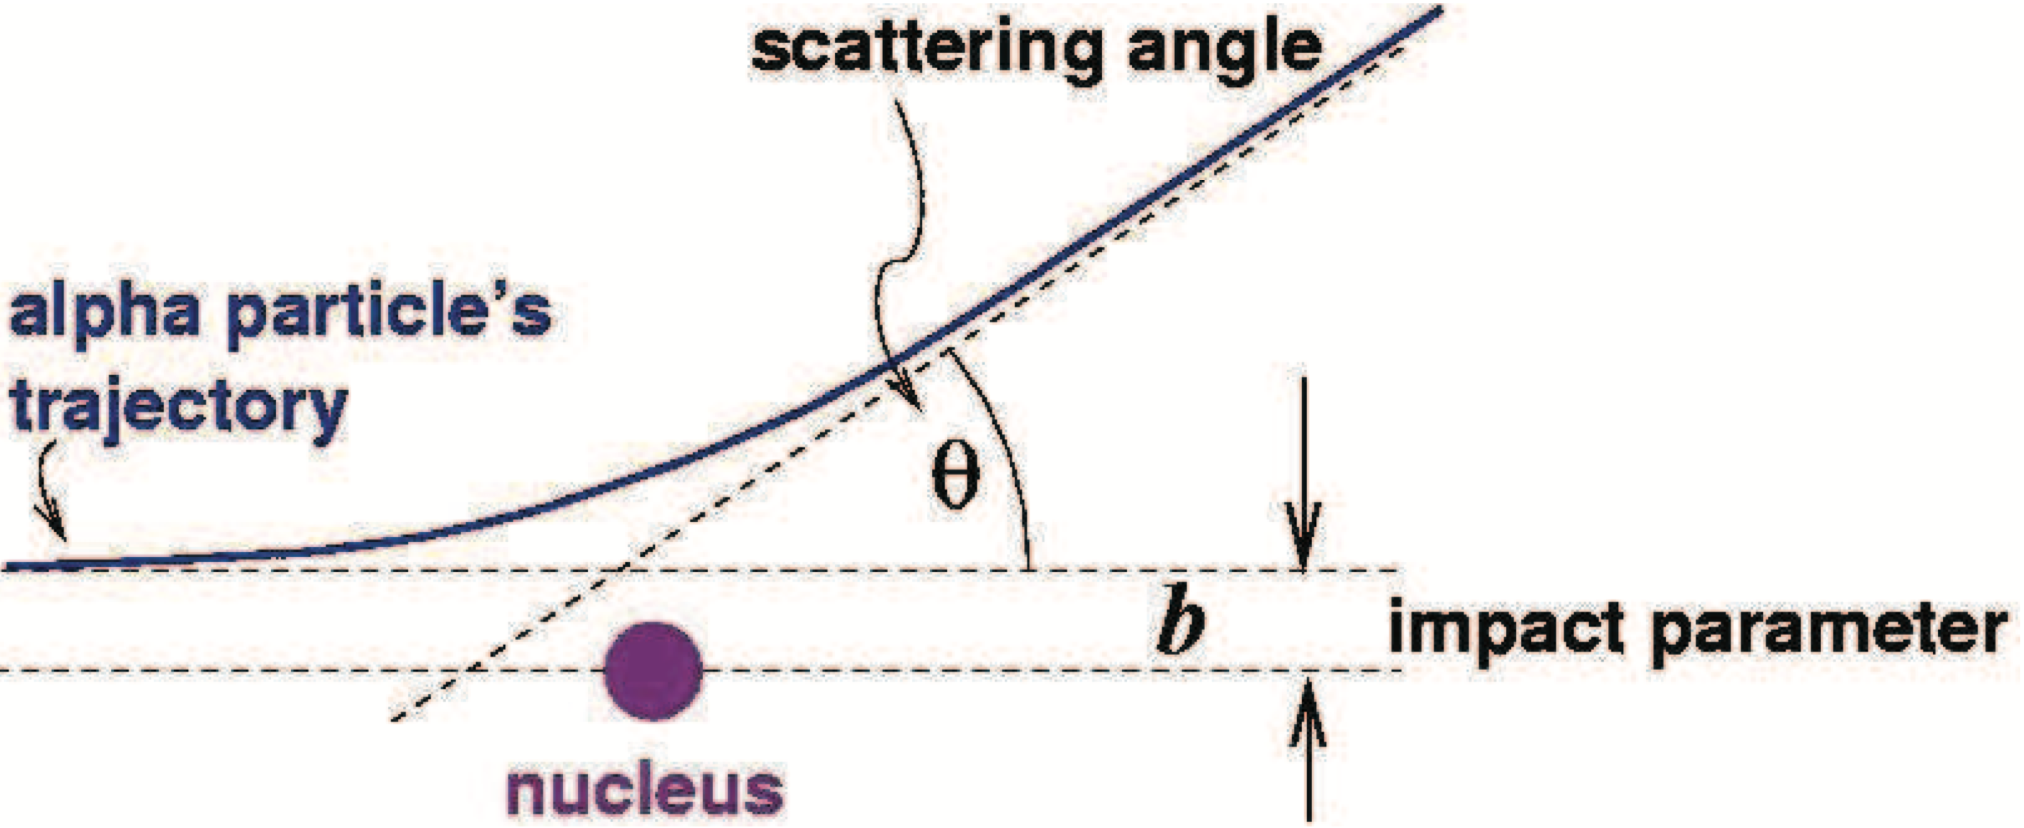
\includegraphics[width=0.8\textwidth]{../images/impactParam.png}
\end{figure}

These 2 values are linked with the following equation$^{\cite{ben-zion_2015}}$:
\[ b(\theta) = \frac{zZe^{2}}{4\pi \epsilon_{0} mv_{0}^{2}}\cot(\frac{\theta}{2}) \]
- \(b(\theta)\): impact parameter - \(\theta\): scattering angle -
\(z\): charge of alpha particle as a multiple of \(e\) - \(Z\): charge
of nucleus as a multiple of \(e\) - \(m\): mass of the alpha particle -
\(v_{0}\): initial speed of the alpha particle

\hypertarget{initial-speed}{%
\subsubsection*{Initial Speed}\label{initial-speed}}

As a quick interlude, we will work out what the initial speed of the
alpha particle was in the original experiment, so we can use it in our
model. Geiger and Marsden used a radium source to produce radon-222 gas,
which emitted the alpha particles. radon-222 decays to polonium-218.
From this we can calculate the gained energy of the alpha particle.
Using \(E=mc^{2}\), the gained KE is calulated:
\[ \Delta KE = M_{r}c^{2} - (M_{p}+M_{\alpha})c^{2} \] Where \(M_{r}\)
is the mass of radon-222, \(222.0175763u\), \(M_{p}\) is the mass of
polonium-218, \(218.0089730u\), and \(M_{\alpha}\) is the mass of an
alpha particle, \(4.001506179127u\). From this, we get a change in
energy of \(~6.6MeV\). Finally, using the equation
\(KE = \frac{1}{2}mv^{2}\) and our value for mass of the alpha particle,
we get a speed of \(1.9\times 10^{7}ms^{-1}\). This is also stored in
the ParticleType enum.

Now that we know the initial speed, we can plug the known values in to
get the following relationship:

\[ b(\theta) = K\cot(\frac{\theta}{2}) \] where
\(K = 1.52142\times 10^{-14}\).

Now, we can run the simulation and compare it to this relationship.

The relevant data values for the gold atom and alpha particle are
already stored in the ParticleType enum. The rest of the data is
determined as follows.

\begin{itemize}
\tightlist
\item
  activity: \(3.7\times 10^{9}\)

  \begin{itemize}
  \tightlist
  \item
    The same as the activity of the radium in the original gold foil
    experiment.
  \end{itemize}
\item
  rMax: 1e-12

  \begin{itemize}
  \tightlist
  \item
    This is arbitrarily chosen, and only affects the spread of the
    results.
  \end{itemize}
\item
  l: 0

  \begin{itemize}
  \tightlist
  \item
    l is 0 for single atom model
  \end{itemize}
\item
  t: 0

  \begin{itemize}
  \tightlist
  \item
    same as above
  \end{itemize}
\item
  d: 1e-6

  \begin{itemize}
  \tightlist
  \item
    also arbitrarily chosen to balance accuracy and speed.
  \end{itemize}
\end{itemize}

We will simulate 5000 particles being emitted.

    \begin{tcolorbox}[breakable, size=fbox, boxrule=1pt, pad at break*=1mm,colback=cellbackground, colframe=cellborder]
\prompt{In}{incolor}{367}{\boxspacing}
\begin{Verbatim}[commandchars=\\\{\}]
\PY{n}{goldAtom} \PY{o}{=} \PY{n}{RutherfordSystem}\PY{p}{(}\PY{n}{activity}\PY{o}{=}\PY{l+m+mf}{3.7e9}\PY{p}{,} 
                            \PY{n}{rMax}\PY{o}{=}\PY{l+m+mf}{1e\PYZhy{}12}\PY{p}{,} 
                            \PY{n}{l}\PY{o}{=}\PY{l+m+mi}{0}\PY{p}{,} 
                            \PY{n}{t}\PY{o}{=}\PY{l+m+mi}{0}\PY{p}{,} 
                            \PY{n}{d}\PY{o}{=}\PY{l+m+mf}{1e\PYZhy{}6}\PY{p}{,} 
                            \PY{n}{particleType}\PY{o}{=}\PY{n}{ParticleType}\PY{o}{.}\PY{n}{ALPHA}\PY{p}{,} 
                            \PY{n}{nucleusType}\PY{o}{=}\PY{n}{ParticleType}\PY{o}{.}\PY{n}{GOLD}\PY{p}{)}

                            
\PY{n}{results} \PY{o}{=} \PY{n}{goldAtom}\PY{o}{.}\PY{n}{multiSim}\PY{p}{(}\PY{l+m+mi}{5000}\PY{p}{)}
\end{Verbatim}
\end{tcolorbox}


\hypertarget{scattering-distribution}{%
\subsubsection{Scattering Distribution}\label{scattering-distribution-single}}

First, we can check if the scattering angles fits with Rutherford's
experiments; that is, most particles have a very small angle, but a
small amount scatter across a large angle.

    \begin{tcolorbox}[breakable, size=fbox, boxrule=1pt, pad at break*=1mm,colback=cellbackground, colframe=cellborder]
\prompt{In}{incolor}{368}{\boxspacing}
\begin{Verbatim}[commandchars=\\\{\}]
\PY{k+kn}{import} \PY{n+nn}{matplotlib}\PY{n+nn}{.}\PY{n+nn}{pyplot} \PY{k}{as} \PY{n+nn}{plt}
\PY{o}{\PYZpc{}}\PY{k}{matplotlib} inline

\PY{n}{hist} \PY{o}{=} \PY{n}{plt}\PY{o}{.}\PY{n}{hist}\PY{p}{(}\PY{n}{results}\PY{p}{[}\PY{l+s+s2}{\PYZdq{}}\PY{l+s+s2}{angles}\PY{l+s+s2}{\PYZdq{}}\PY{p}{]}\PY{p}{,} \PY{l+m+mi}{36}\PY{p}{)}
\PY{n}{plt}\PY{o}{.}\PY{n}{xlabel}\PY{p}{(}\PY{l+s+s1}{\PYZsq{}}\PY{l+s+s1}{Angles}\PY{l+s+s1}{\PYZsq{}}\PY{p}{)}
\PY{n}{plt}\PY{o}{.}\PY{n}{ylabel}\PY{p}{(}\PY{l+s+s1}{\PYZsq{}}\PY{l+s+s1}{Frequency}\PY{l+s+s1}{\PYZsq{}}\PY{p}{)}
\PY{n}{plt}\PY{o}{.}\PY{n}{title}\PY{p}{(}\PY{l+s+s1}{\PYZsq{}}\PY{l+s+s1}{Histogram of Angles}\PY{l+s+s1}{\PYZsq{}}\PY{p}{)}
\PY{n}{plt}\PY{o}{.}\PY{n}{xlim}\PY{p}{(}\PY{l+m+mi}{0}\PY{p}{,} \PY{l+m+mi}{180}\PY{p}{)}
\PY{n}{plt}\PY{o}{.}\PY{n}{grid}\PY{p}{(}\PY{k+kc}{True}\PY{p}{)}

\PY{n}{plt}\PY{o}{.}\PY{n}{show}\PY{p}{(}\PY{p}{)}
\end{Verbatim}
\end{tcolorbox}

    \begin{center}
    \adjustimage{max size={0.9\linewidth}{0.9\paperheight}}{../outputs/singleAtomHist.png}
    \end{center}
    { \hspace*{\fill} \\}
    
    As we can see, the model fits well. a large majority of particle barely
scattered at all, most less than \(5^{\circ}\), but a small amount had a
large scattering angle, with some surpassing \(140^{\circ}\).

    \hypertarget{impact-parameter-relationship}{%
\subsubsection{Impact Parameter
Relationship}\label{impact-parameter-relationship}}

Next, we can analyze the relationship we looked at earlier. Firstly, to
plot angle against impact parameter, we need an equation for the angle
in terms of the impact parameter, so we need to invert the function, and
code it.

\[ \theta (b) = 2\arctan(\frac{K}{b}) \]

    \begin{tcolorbox}[breakable, size=fbox, boxrule=1pt, pad at break*=1mm,colback=cellbackground, colframe=cellborder]
\prompt{In}{incolor}{369}{\boxspacing}
\begin{Verbatim}[commandchars=\\\{\}]
\PY{k}{def} \PY{n+nf}{scatterAngle}\PY{p}{(}\PY{n}{b}\PY{p}{)}\PY{p}{:}
    \PY{k}{return} \PY{n}{np}\PY{o}{.}\PY{n}{degrees}\PY{p}{(}\PY{n}{np}\PY{o}{.}\PY{n}{arctan}\PY{p}{(}\PY{l+m+mf}{1.52109e\PYZhy{}14}\PY{o}{*}\PY{p}{(}\PY{n}{b}\PY{o}{*}\PY{o}{*}\PY{o}{\PYZhy{}}\PY{l+m+mi}{1}\PY{p}{)}\PY{p}{)}\PY{o}{*}\PY{l+m+mi}{2}\PY{p}{)}
\end{Verbatim}
\end{tcolorbox}

    Now we can plot our results against the expected results.

    \begin{tcolorbox}[breakable, size=fbox, boxrule=1pt, pad at break*=1mm,colback=cellbackground, colframe=cellborder]
\prompt{In}{incolor}{370}{\boxspacing}
\begin{Verbatim}[commandchars=\\\{\}]
\PY{n}{fig} \PY{o}{=} \PY{n}{plt}\PY{o}{.}\PY{n}{figure}\PY{p}{(}\PY{p}{)}
\PY{n}{ax} \PY{o}{=} \PY{n}{fig}\PY{o}{.}\PY{n}{add\PYZus{}subplot}\PY{p}{(}\PY{p}{)}
\PY{n}{plt}\PY{o}{.}\PY{n}{title}\PY{p}{(}\PY{l+s+s2}{\PYZdq{}}\PY{l+s+s2}{Scattering angle against Impact parameter}\PY{l+s+s2}{\PYZdq{}}\PY{p}{)}
\PY{n}{plt}\PY{o}{.}\PY{n}{xlabel}\PY{p}{(}\PY{l+s+s2}{\PYZdq{}}\PY{l+s+s2}{Scatering Angle}\PY{l+s+s2}{\PYZdq{}}\PY{p}{)}
\PY{n}{plt}\PY{o}{.}\PY{n}{ylabel}\PY{p}{(}\PY{l+s+s2}{\PYZdq{}}\PY{l+s+s2}{Impact Parameter}\PY{l+s+s2}{\PYZdq{}}\PY{p}{)}


\PY{n}{ax}\PY{o}{.}\PY{n}{scatter}\PY{p}{(}\PY{n}{results}\PY{p}{[}\PY{l+s+s2}{\PYZdq{}}\PY{l+s+s2}{offsets}\PY{l+s+s2}{\PYZdq{}}\PY{p}{]}\PY{p}{,} \PY{n}{results}\PY{p}{[}\PY{l+s+s2}{\PYZdq{}}\PY{l+s+s2}{angles}\PY{l+s+s2}{\PYZdq{}}\PY{p}{]}\PY{p}{,} \PY{n}{marker}\PY{o}{=}\PY{l+s+s2}{\PYZdq{}}\PY{l+s+s2}{.}\PY{l+s+s2}{\PYZdq{}}\PY{p}{,} \PY{n}{label}\PY{o}{=}\PY{l+s+s2}{\PYZdq{}}\PY{l+s+s2}{simulation}\PY{l+s+s2}{\PYZdq{}}\PY{p}{)}

\PY{n}{x} \PY{o}{=} \PY{n}{np}\PY{o}{.}\PY{n}{linspace}\PY{p}{(}\PY{l+m+mf}{1e\PYZhy{}20}\PY{p}{,} \PY{l+m+mf}{1e\PYZhy{}12}\PY{p}{,} \PY{l+m+mi}{1000}\PY{p}{)}
\PY{n}{ax}\PY{o}{.}\PY{n}{plot}\PY{p}{(}\PY{n}{x}\PY{p}{,} \PY{n}{scatterAngle}\PY{p}{(}\PY{n}{x}\PY{p}{)}\PY{p}{,} \PY{n}{c}\PY{o}{=}\PY{l+s+s2}{\PYZdq{}}\PY{l+s+s2}{orange}\PY{l+s+s2}{\PYZdq{}}\PY{p}{,} \PY{n}{label}\PY{o}{=}\PY{l+s+s2}{\PYZdq{}}\PY{l+s+s2}{equation}\PY{l+s+s2}{\PYZdq{}}\PY{p}{)}

\PY{n}{ax}\PY{o}{.}\PY{n}{legend}\PY{p}{(}\PY{p}{)}
\PY{n}{plt}\PY{o}{.}\PY{n}{show}\PY{p}{(}\PY{p}{)}
\end{Verbatim}
\end{tcolorbox}

    \begin{center}
    \adjustimage{max size={0.9\linewidth}{0.9\paperheight}}{../outputs/thetaAgainstB.png}
    \end{center}
    { \hspace*{\fill} \\}
    
    The line fits perfectly with the data, which shows that this equation
linking impact parameter and scattering angle is correct. To ensure
this, I performed residual analysis on the relationship. This involves
calculating the residual for each point, and plotting it against the
impact parameter. The residual is calulated as follows:

\[ e = \theta - \hat{\theta} \]

where e is the residual, \(\theta\) is the angle from the simulation and
\(\hat{\theta}\) is the calculated angle.

    \begin{tcolorbox}[breakable, size=fbox, boxrule=1pt, pad at break*=1mm,colback=cellbackground, colframe=cellborder]
\prompt{In}{incolor}{371}{\boxspacing}
\begin{Verbatim}[commandchars=\\\{\}]
\PY{n}{residual} \PY{o}{=} \PY{p}{[}\PY{p}{]}
\PY{k}{for} \PY{n}{b}\PY{p}{,} \PY{n}{angle} \PY{o+ow}{in} \PY{n+nb}{zip}\PY{p}{(}\PY{n}{results}\PY{p}{[}\PY{l+s+s2}{\PYZdq{}}\PY{l+s+s2}{offsets}\PY{l+s+s2}{\PYZdq{}}\PY{p}{]}\PY{p}{,} \PY{n}{results}\PY{p}{[}\PY{l+s+s2}{\PYZdq{}}\PY{l+s+s2}{angles}\PY{l+s+s2}{\PYZdq{}}\PY{p}{]}\PY{p}{)}\PY{p}{:}
    \PY{n}{residual}\PY{o}{.}\PY{n}{append}\PY{p}{(}\PY{n}{angle}\PY{o}{\PYZhy{}}\PY{n}{scatterAngle}\PY{p}{(}\PY{n}{b}\PY{p}{)}\PY{p}{)}

\PY{n}{fig} \PY{o}{=} \PY{n}{plt}\PY{o}{.}\PY{n}{figure}\PY{p}{(}\PY{p}{)}
\PY{n}{plt}\PY{o}{.}\PY{n}{title}\PY{p}{(}\PY{l+s+s2}{\PYZdq{}}\PY{l+s+s2}{Residual Analysis}\PY{l+s+s2}{\PYZdq{}}\PY{p}{)}
\PY{n}{plt}\PY{o}{.}\PY{n}{xlabel}\PY{p}{(}\PY{l+s+s2}{\PYZdq{}}\PY{l+s+s2}{Impact Parameter}\PY{l+s+s2}{\PYZdq{}}\PY{p}{)}
\PY{n}{plt}\PY{o}{.}\PY{n}{ylabel}\PY{p}{(}\PY{l+s+s2}{\PYZdq{}}\PY{l+s+s2}{Residual}\PY{l+s+s2}{\PYZdq{}}\PY{p}{)}
\PY{n}{plt}\PY{o}{.}\PY{n}{scatter}\PY{p}{(}\PY{n}{results}\PY{p}{[}\PY{l+s+s2}{\PYZdq{}}\PY{l+s+s2}{offsets}\PY{l+s+s2}{\PYZdq{}}\PY{p}{]}\PY{p}{,} \PY{n}{residual}\PY{p}{)}
\PY{n}{plt}\PY{o}{.}\PY{n}{show}\PY{p}{(}\PY{p}{)}
\end{Verbatim}
\end{tcolorbox}

    \begin{center}
    \adjustimage{max size={0.9\linewidth}{0.9\paperheight}}{../outputs/residualAnal.png}
    \end{center}
    { \hspace*{\fill} \\}
    
    While there is a quirk in the residual at around \(10^{-14}\) m, this
can probably be explained with how the timestep lines up with the
closest approach to the nucleus. Importantly, the max error is only
\(0.16^{\circ}\), and most are a lot less than that, and so I can
confidently conclude the equation described accurately models the
relationship between scattering angle and impact parameter.

\hypertarget{trajectory}{%
\subsubsection{Trajectory}\label{trajectory}}

Finally, we can have a look at the trajectory of a single alpha
particle, to ensure behaviour is as expected. I will use a value of
\(b=1.5210857\times 10^{-14}\), as this should produce a \(90^{\circ}\)
angle, according to the equation.

    \begin{tcolorbox}[breakable, size=fbox, boxrule=1pt, pad at break*=1mm,colback=cellbackground, colframe=cellborder]
\prompt{In}{incolor}{113}{\boxspacing}
\begin{Verbatim}[commandchars=\\\{\}]
\PY{n}{singleSim} \PY{o}{=} \PY{n}{goldAtom}\PY{o}{.}\PY{n}{singleSim}\PY{p}{(}\PY{n}{b}\PY{o}{=}\PY{l+m+mf}{1.5210857e\PYZhy{}14}\PY{p}{)}
\PY{n+nb}{print}\PY{p}{(}\PY{n}{singleSim}\PY{p}{[}\PY{l+s+s2}{\PYZdq{}}\PY{l+s+s2}{angle}\PY{l+s+s2}{\PYZdq{}}\PY{p}{]}\PY{p}{)}

\PY{n}{fig} \PY{o}{=} \PY{n}{plt}\PY{o}{.}\PY{n}{figure}\PY{p}{(}\PY{p}{)}
\PY{n}{ax} \PY{o}{=} \PY{n}{fig}\PY{o}{.}\PY{n}{add\PYZus{}subplot}\PY{p}{(}\PY{n}{projection}\PY{o}{=}\PY{l+s+s1}{\PYZsq{}}\PY{l+s+s1}{3d}\PY{l+s+s1}{\PYZsq{}}\PY{p}{)}
\PY{n}{ax}\PY{o}{.}\PY{n}{scatter}\PY{p}{(}\PY{n}{singleSim}\PY{p}{[}\PY{l+s+s2}{\PYZdq{}}\PY{l+s+s2}{positions}\PY{l+s+s2}{\PYZdq{}}\PY{p}{]}\PY{p}{[}\PY{o}{.}\PY{o}{.}\PY{o}{.}\PY{p}{,}\PY{l+m+mi}{0}\PY{p}{]}\PY{p}{,} \PY{n}{singleSim}\PY{p}{[}\PY{l+s+s2}{\PYZdq{}}\PY{l+s+s2}{positions}\PY{l+s+s2}{\PYZdq{}}\PY{p}{]}\PY{p}{[}\PY{o}{.}\PY{o}{.}\PY{o}{.}\PY{p}{,}\PY{l+m+mi}{1}\PY{p}{]}\PY{p}{,} \PY{n}{singleSim}\PY{p}{[}\PY{l+s+s2}{\PYZdq{}}\PY{l+s+s2}{positions}\PY{l+s+s2}{\PYZdq{}}\PY{p}{]}\PY{p}{[}\PY{o}{.}\PY{o}{.}\PY{o}{.}\PY{p}{,}\PY{l+m+mi}{2}\PY{p}{]}\PY{p}{,} \PY{n}{marker} \PY{o}{=} \PY{l+s+s2}{\PYZdq{}}\PY{l+s+s2}{o}\PY{l+s+s2}{\PYZdq{}}\PY{p}{)}
\PY{k}{for} \PY{n}{nucleus} \PY{o+ow}{in} \PY{n}{goldAtom}\PY{o}{.}\PY{n}{nuclei}\PY{p}{:}
    \PY{n}{ax}\PY{o}{.}\PY{n}{scatter}\PY{p}{(}\PY{n}{nucleus}\PY{o}{.}\PY{n}{position}\PY{p}{[}\PY{l+m+mi}{0}\PY{p}{]}\PY{p}{,} \PY{n}{nucleus}\PY{o}{.}\PY{n}{position}\PY{p}{[}\PY{l+m+mi}{1}\PY{p}{]}\PY{p}{,} \PY{n}{nucleus}\PY{o}{.}\PY{n}{position}\PY{p}{[}\PY{l+m+mi}{2}\PY{p}{]}\PY{p}{,} \PY{n}{marker} \PY{o}{=} \PY{l+s+s2}{\PYZdq{}}\PY{l+s+s2}{X}\PY{l+s+s2}{\PYZdq{}}\PY{p}{)}
\PY{n}{plt}\PY{o}{.}\PY{n}{show}\PY{p}{(}\PY{p}{)}
\end{Verbatim}
\end{tcolorbox}

    \begin{Verbatim}[commandchars=\\\{\}]
89.84380427965971
    \end{Verbatim}

    \begin{center}
    \adjustimage{max size={0.9\linewidth}{0.9\paperheight}}{../outputs/trajectory.png}
    \end{center}
    { \hspace*{\fill} \\}
    
    The trajectory of the particle is as expected. If ran seperately the
graph is interactive, and the timestep jumps can be seen: these are
sufficiently close together for an accurate result. The angle is also
only 0.16\% off, which is more than accurate enough for our uses.

    \hypertarget{d-lattice}{%
\subsection{2D Lattice}\label{d-lattice}}

The next stage of the simulation is creating a 2D lattice. This is done
by setting the thickness of the lattice to 0. With this simulation, we
will analyse the accuracy of the original experiments, and the effect
the material has on the results. We will use the same initialization
data as the single atom simulation, with a couple key differences: rMax
and l. Since the scale of the original experiment in terms of the number
of atoms is too large to feasibly simulate, I had to compromise and find
a balance between accuracy and efficiency. rMax was set to just under
half this value, to cover most of the lattice.

I will run a simulation of 1000 particles.

    \begin{tcolorbox}[breakable, size=fbox, boxrule=1pt, pad at break*=1mm,colback=cellbackground, colframe=cellborder]
\prompt{In}{incolor}{146}{\boxspacing}
\begin{Verbatim}[commandchars=\\\{\}]
\PY{n}{goldLattice} \PY{o}{=} \PY{n}{RutherfordSystem}\PY{p}{(}\PY{n}{activity}\PY{o}{=}\PY{l+m+mf}{3.7e9}\PY{p}{,} 
                               \PY{n}{rMax}\PY{o}{=}\PY{l+m+mf}{2.9e\PYZhy{}9}\PY{p}{,} 
                               \PY{n}{l}\PY{o}{=}\PY{l+m+mf}{6e\PYZhy{}9}\PY{p}{,} 
                               \PY{n}{t}\PY{o}{=}\PY{l+m+mi}{0}\PY{p}{,} 
                               \PY{n}{d}\PY{o}{=}\PY{l+m+mf}{1e\PYZhy{}6}\PY{p}{,} 
                               \PY{n}{particleType}\PY{o}{=}\PY{n}{ParticleType}\PY{o}{.}\PY{n}{ALPHA}\PY{p}{,} 
                               \PY{n}{nucleusType}\PY{o}{=}\PY{n}{ParticleType}\PY{o}{.}\PY{n}{GOLD}\PY{p}{)}

\PY{n}{results} \PY{o}{=} \PY{n}{goldLattice}\PY{o}{.}\PY{n}{multiSim}\PY{p}{(}\PY{l+m+mi}{1000}\PY{p}{)}
\end{Verbatim}
\end{tcolorbox}

\hypertarget{lattice}{%
\subsubsection{Lattice}\label{lattice}}

Firstly I will check the formation of the lattice:

    \begin{tcolorbox}[breakable, size=fbox, boxrule=1pt, pad at break*=1mm,colback=cellbackground, colframe=cellborder]
\prompt{In}{incolor}{159}{\boxspacing}
\begin{Verbatim}[commandchars=\\\{\}]
\PY{n}{fig} \PY{o}{=} \PY{n}{plt}\PY{o}{.}\PY{n}{figure}\PY{p}{(}\PY{p}{)}
\PY{n}{ax} \PY{o}{=} \PY{n}{fig}\PY{o}{.}\PY{n}{add\PYZus{}subplot}\PY{p}{(}\PY{n}{projection}\PY{o}{=}\PY{l+s+s2}{\PYZdq{}}\PY{l+s+s2}{3d}\PY{l+s+s2}{\PYZdq{}}\PY{p}{)}
\PY{n}{plt}\PY{o}{.}\PY{n}{title}\PY{p}{(}\PY{l+s+s2}{\PYZdq{}}\PY{l+s+s2}{2D Lattice}\PY{l+s+s2}{\PYZdq{}}\PY{p}{)}

\PY{k}{for} \PY{n}{nucleus} \PY{o+ow}{in} \PY{n}{goldLattice}\PY{o}{.}\PY{n}{nuclei}\PY{p}{:}
    \PY{n}{plt}\PY{o}{.}\PY{n}{scatter}\PY{p}{(}\PY{n}{nucleus}\PY{o}{.}\PY{n}{position}\PY{p}{[}\PY{l+m+mi}{0}\PY{p}{]}\PY{p}{,} \PY{n}{nucleus}\PY{o}{.}\PY{n}{position}\PY{p}{[}\PY{l+m+mi}{1}\PY{p}{]}\PY{p}{,} \PY{n}{nucleus}\PY{o}{.}\PY{n}{position}\PY{p}{[}\PY{l+m+mi}{2}\PY{p}{]}\PY{p}{,} \PY{n}{c}\PY{o}{=}\PY{l+s+s2}{\PYZdq{}}\PY{l+s+s2}{blue}\PY{l+s+s2}{\PYZdq{}}\PY{p}{,} \PY{n}{marker}\PY{o}{=}\PY{l+s+s2}{\PYZdq{}}\PY{l+s+s2}{X}\PY{l+s+s2}{\PYZdq{}}\PY{p}{)}

\PY{n}{plt}\PY{o}{.}\PY{n}{show}\PY{p}{(}\PY{p}{)}
\end{Verbatim}
\end{tcolorbox}

    \begin{center}
    \adjustimage{max size={0.9\linewidth}{0.9\paperheight}}{../outputs/2DLattice.png}
    \end{center}
    { \hspace*{\fill} \\}
    
    I can see that the lattice is formed in the correct shape.

\hypertarget{scattering-distribution}{%
\subsubsection{Scattering Distribution}\label{scattering-distribution}}

Next I can look at the distribution of scattering angles. Again,
Rutherford observed that a large majority of particles barely scatter,
while a small amount deflect a large angle.

    \begin{tcolorbox}[breakable, size=fbox, boxrule=1pt, pad at break*=1mm,colback=cellbackground, colframe=cellborder]
\prompt{In}{incolor}{160}{\boxspacing}
\begin{Verbatim}[commandchars=\\\{\}]
\PY{n}{hist} \PY{o}{=} \PY{n}{plt}\PY{o}{.}\PY{n}{hist}\PY{p}{(}\PY{n}{results}\PY{p}{[}\PY{l+s+s2}{\PYZdq{}}\PY{l+s+s2}{angles}\PY{l+s+s2}{\PYZdq{}}\PY{p}{]}\PY{p}{,} \PY{l+m+mi}{36}\PY{p}{)}
\PY{n}{plt}\PY{o}{.}\PY{n}{xlabel}\PY{p}{(}\PY{l+s+s1}{\PYZsq{}}\PY{l+s+s1}{Angles}\PY{l+s+s1}{\PYZsq{}}\PY{p}{)}
\PY{n}{plt}\PY{o}{.}\PY{n}{ylabel}\PY{p}{(}\PY{l+s+s1}{\PYZsq{}}\PY{l+s+s1}{Frequency}\PY{l+s+s1}{\PYZsq{}}\PY{p}{)}
\PY{n}{plt}\PY{o}{.}\PY{n}{title}\PY{p}{(}\PY{l+s+s1}{\PYZsq{}}\PY{l+s+s1}{Histogram of Angles}\PY{l+s+s1}{\PYZsq{}}\PY{p}{)}
\PY{n}{plt}\PY{o}{.}\PY{n}{grid}\PY{p}{(}\PY{k+kc}{True}\PY{p}{)}

\PY{n}{plt}\PY{o}{.}\PY{n}{show}\PY{p}{(}\PY{p}{)}
\end{Verbatim}
\end{tcolorbox}

    \begin{center}
    \adjustimage{max size={0.9\linewidth}{0.9\paperheight}}{../outputs/2DHist.png}
    \end{center}
    { \hspace*{\fill} \\}
    
    These results are a lot less conclusive than the single atom. This is
because of the limitation of the efficiency of the model; in order to
gain more conclusive results, either the length of the lattice or the
number of alpha particles would have to be increased, which is not
feasible with the time constraints. However, we can still see
Rutherford's observations in work here; most angles are below
\(0.1^{\circ}\), but some reach up to \(0.3^{\circ}\). While these are
small angles, the same conclusions can be made.

    \hypertarget{effect-of-material}{%
\subsubsection{Effect of Material}\label{effect-of-material}}

To test the effect of material on scattering distribution, I will run the simulation with lead,
heavier than gold, and tin, lighter than gold. Lead should result in
more scattering than tin, as it has a higher charge per nucleus. Again,
the data for each material is already in the ParticleType Enum.

    \begin{tcolorbox}[breakable, size=fbox, boxrule=1pt, pad at break*=1mm,colback=cellbackground, colframe=cellborder]
\prompt{In}{incolor}{ }{\boxspacing}
\begin{Verbatim}[commandchars=\\\{\}]
\PY{n}{goldLattice}\PY{o}{.}\PY{n}{changeNucleus}\PY{p}{(}\PY{n}{nucleusType}\PY{o}{=}\PY{n}{ParticleType}\PY{o}{.}\PY{n}{LEAD}\PY{p}{)}
\PY{n}{leadResults} \PY{o}{=} \PY{n}{goldLattice}\PY{o}{.}\PY{n}{multiSim}\PY{p}{(}\PY{n}{num}\PY{o}{=}\PY{l+m+mi}{100}\PY{p}{)}

\PY{n}{goldLattice}\PY{o}{.}\PY{n}{changeNucleus}\PY{p}{(}\PY{n}{nucleusType}\PY{o}{=}\PY{n}{ParticleType}\PY{o}{.}\PY{n}{TIN}\PY{p}{)}
\PY{n}{tinResults} \PY{o}{=} \PY{n}{goldLattice}\PY{o}{.}\PY{n}{multiSim}\PY{p}{(}\PY{n}{num}\PY{o}{=}\PY{l+m+mi}{100}\PY{p}{)}
\end{Verbatim}
\end{tcolorbox}

    \begin{tcolorbox}[breakable, size=fbox, boxrule=1pt, pad at break*=1mm,colback=cellbackground, colframe=cellborder]
\prompt{In}{incolor}{301}{\boxspacing}
\begin{Verbatim}[commandchars=\\\{\}]
\PY{n}{plt}\PY{o}{.}\PY{n}{subplot}\PY{p}{(}\PY{l+m+mi}{211}\PY{p}{)}
\PY{n}{plt}\PY{o}{.}\PY{n}{hist}\PY{p}{(}\PY{n}{leadResults}\PY{p}{[}\PY{l+s+s2}{\PYZdq{}}\PY{l+s+s2}{angles}\PY{l+s+s2}{\PYZdq{}}\PY{p}{]}\PY{p}{,} \PY{l+m+mi}{36}\PY{p}{)}
\PY{n}{plt}\PY{o}{.}\PY{n}{xlabel}\PY{p}{(}\PY{l+s+s1}{\PYZsq{}}\PY{l+s+s1}{Angles}\PY{l+s+s1}{\PYZsq{}}\PY{p}{)}
\PY{n}{plt}\PY{o}{.}\PY{n}{ylabel}\PY{p}{(}\PY{l+s+s1}{\PYZsq{}}\PY{l+s+s1}{Frequency}\PY{l+s+s1}{\PYZsq{}}\PY{p}{)}
\PY{n}{plt}\PY{o}{.}\PY{n}{text}\PY{p}{(}\PY{l+m+mi}{0}\PY{p}{,} \PY{l+m+mi}{10}\PY{p}{,} \PY{l+s+s2}{\PYZdq{}}\PY{l+s+s2}{Lead}\PY{l+s+s2}{\PYZdq{}}\PY{p}{)}
\PY{n}{plt}\PY{o}{.}\PY{n}{title}\PY{p}{(}\PY{l+s+s1}{\PYZsq{}}\PY{l+s+s1}{Histogram of Angles}\PY{l+s+s1}{\PYZsq{}}\PY{p}{)}
\PY{n}{plt}\PY{o}{.}\PY{n}{xlim}\PY{p}{(}\PY{l+m+mi}{0}\PY{p}{,} \PY{l+m+mf}{0.2}\PY{p}{)}
\PY{n}{plt}\PY{o}{.}\PY{n}{grid}\PY{p}{(}\PY{k+kc}{True}\PY{p}{)}

\PY{n}{plt}\PY{o}{.}\PY{n}{subplot}\PY{p}{(}\PY{l+m+mi}{212}\PY{p}{)}
\PY{n}{plt}\PY{o}{.}\PY{n}{hist}\PY{p}{(}\PY{n}{tinResults}\PY{p}{[}\PY{l+s+s2}{\PYZdq{}}\PY{l+s+s2}{angles}\PY{l+s+s2}{\PYZdq{}}\PY{p}{]}\PY{p}{,} \PY{l+m+mi}{20}\PY{p}{)}
\PY{n}{plt}\PY{o}{.}\PY{n}{xlabel}\PY{p}{(}\PY{l+s+s1}{\PYZsq{}}\PY{l+s+s1}{Angles}\PY{l+s+s1}{\PYZsq{}}\PY{p}{)}
\PY{n}{plt}\PY{o}{.}\PY{n}{ylabel}\PY{p}{(}\PY{l+s+s1}{\PYZsq{}}\PY{l+s+s1}{Frequency}\PY{l+s+s1}{\PYZsq{}}\PY{p}{)}
\PY{n}{plt}\PY{o}{.}\PY{n}{text}\PY{p}{(}\PY{l+m+mi}{0}\PY{p}{,} \PY{l+m+mi}{10}\PY{p}{,} \PY{l+s+s2}{\PYZdq{}}\PY{l+s+s2}{Tin}\PY{l+s+s2}{\PYZdq{}}\PY{p}{)}
\PY{n}{plt}\PY{o}{.}\PY{n}{xlim}\PY{p}{(}\PY{l+m+mi}{0}\PY{p}{,} \PY{l+m+mf}{0.2}\PY{p}{)}
\PY{n}{plt}\PY{o}{.}\PY{n}{grid}\PY{p}{(}\PY{k+kc}{True}\PY{p}{)}

\PY{n}{plt}\PY{o}{.}\PY{n}{show}\PY{p}{(}\PY{p}{)}
\end{Verbatim}
\end{tcolorbox}

    \begin{center}
    \adjustimage{max size={0.9\linewidth}{0.9\paperheight}}{../outputs/material.png}
    \end{center}
    { \hspace*{\fill} \\}
    
    the scattering of tin is significantly less than that of lead, which is
expected. What is interesting here is the distribution of lead
scattering is more spread out than tin, rather than just having more
particles that scatter more. This makes sense, as all particles feel an
electric force even if it is small, so a larger charge and therefore a
larger force will spread out the small deflections.

    \hypertarget{d-lattice}{%
\subsection{3D Lattice}\label{d-lattice}}

    The final stage of this model is to create a 3D lattice. This is done by
setting the thickness and side length of the lattice. In theh original
experiment, a thickness of \(10^{7}\) m was used. However this
translates to \textasciitilde245 layers, which is too much for the model
to simulate. Instead, I will use a thickness of \(10^{-9}\) m. The rest
of the parameters will be identtical to the 2D lattice simulation.
Additionally, I will analyse Rutherford's proposed relationship between
thickness and scattering distribution by running smaller tests at
varying thicknesses.

    \begin{tcolorbox}[breakable, size=fbox, boxrule=1pt, pad at break*=1mm,colback=cellbackground, colframe=cellborder]
\prompt{In}{incolor}{2}{\boxspacing}
\begin{Verbatim}[commandchars=\\\{\}]
\PY{n}{goldLattice} \PY{o}{=} \PY{n}{RutherfordSystem}\PY{p}{(}\PY{n}{activity}\PY{o}{=}\PY{l+m+mf}{3.7e9}\PY{p}{,} 
                               \PY{n}{rMax}\PY{o}{=}\PY{l+m+mf}{2.9e\PYZhy{}9}\PY{p}{,} 
                               \PY{n}{l}\PY{o}{=}\PY{l+m+mf}{6e\PYZhy{}9}\PY{p}{,} 
                               \PY{n}{t}\PY{o}{=}\PY{l+m+mf}{1e\PYZhy{}9}\PY{p}{,} 
                               \PY{n}{d}\PY{o}{=}\PY{l+m+mf}{1e\PYZhy{}6}\PY{p}{,} 
                               \PY{n}{particleType}\PY{o}{=}\PY{n}{ParticleType}\PY{o}{.}\PY{n}{ALPHA}\PY{p}{,} 
                               \PY{n}{nucleusType}\PY{o}{=}\PY{n}{ParticleType}\PY{o}{.}\PY{n}{GOLD}\PY{p}{)}

\PY{n}{results} \PY{o}{=} \PY{n}{goldLattice}\PY{o}{.}\PY{n}{multiSim}\PY{p}{(}\PY{l+m+mi}{500}\PY{p}{)}
\end{Verbatim}
\end{tcolorbox}

    \hypertarget{lattice-visualisation}{%
\subsubsection{Lattice Visualisation}\label{lattice-visualisation}}

First, I will check the Lattice arrangement.

    \begin{tcolorbox}[breakable, size=fbox, boxrule=1pt, pad at break*=1mm,colback=cellbackground, colframe=cellborder]
\prompt{In}{incolor}{28}{\boxspacing}
\begin{Verbatim}[commandchars=\\\{\}]
\PY{n}{fig} \PY{o}{=} \PY{n}{plt}\PY{o}{.}\PY{n}{figure}\PY{p}{(}\PY{p}{)}
\PY{n}{ax} \PY{o}{=} \PY{n}{fig}\PY{o}{.}\PY{n}{add\PYZus{}subplot}\PY{p}{(}\PY{n}{projection}\PY{o}{=}\PY{l+s+s2}{\PYZdq{}}\PY{l+s+s2}{3d}\PY{l+s+s2}{\PYZdq{}}\PY{p}{)}
\PY{n}{plt}\PY{o}{.}\PY{n}{title}\PY{p}{(}\PY{l+s+s2}{\PYZdq{}}\PY{l+s+s2}{3D Lattice}\PY{l+s+s2}{\PYZdq{}}\PY{p}{)}


\PY{k}{for} \PY{n}{i} \PY{o+ow}{in} \PY{n}{goldLattice}\PY{o}{.}\PY{n}{nuclei}\PY{p}{:}
    \PY{n}{ax}\PY{o}{.}\PY{n}{scatter}\PY{p}{(}\PY{n}{i}\PY{o}{.}\PY{n}{position}\PY{p}{[}\PY{l+m+mi}{0}\PY{p}{]}\PY{p}{,} \PY{n}{i}\PY{o}{.}\PY{n}{position}\PY{p}{[}\PY{l+m+mi}{1}\PY{p}{]}\PY{p}{,} \PY{n}{i}\PY{o}{.}\PY{n}{position}\PY{p}{[}\PY{l+m+mi}{2}\PY{p}{]}\PY{p}{,} \PY{n}{c}\PY{o}{=}\PY{l+s+s2}{\PYZdq{}}\PY{l+s+s2}{blue}\PY{l+s+s2}{\PYZdq{}}\PY{p}{,} \PY{n}{marker}\PY{o}{=}\PY{l+s+s2}{\PYZdq{}}\PY{l+s+s2}{X}\PY{l+s+s2}{\PYZdq{}}\PY{p}{)}

\PY{n}{plt}\PY{o}{.}\PY{n}{show}\PY{p}{(}\PY{p}{)}
\end{Verbatim}
\end{tcolorbox}

    \begin{center}
    \adjustimage{max size={0.9\linewidth}{0.9\paperheight}}{../outputs/3DLattice}
    \end{center}
    { \hspace*{\fill} \\}
    
    This is accurate to the face-centered cubic lattice structure of gold,
so we can move on.

    \hypertarget{scattering-distribution}{%
\subsubsection{Scattering Distribution}\label{scattering-distribution1}}

Next, we can look at the scattering distribution of the 3D lattice
simulation.

    \begin{tcolorbox}[breakable, size=fbox, boxrule=1pt, pad at break*=1mm,colback=cellbackground, colframe=cellborder]
\prompt{In}{incolor}{5}{\boxspacing}
\begin{Verbatim}[commandchars=\\\{\}]
\PY{n}{hist} \PY{o}{=} \PY{n}{plt}\PY{o}{.}\PY{n}{hist}\PY{p}{(}\PY{n}{results}\PY{p}{[}\PY{l+s+s2}{\PYZdq{}}\PY{l+s+s2}{angles}\PY{l+s+s2}{\PYZdq{}}\PY{p}{]}\PY{p}{,} \PY{l+m+mi}{36}\PY{p}{)}
\PY{n}{plt}\PY{o}{.}\PY{n}{xlabel}\PY{p}{(}\PY{l+s+s1}{\PYZsq{}}\PY{l+s+s1}{Angles}\PY{l+s+s1}{\PYZsq{}}\PY{p}{)}
\PY{n}{plt}\PY{o}{.}\PY{n}{ylabel}\PY{p}{(}\PY{l+s+s1}{\PYZsq{}}\PY{l+s+s1}{Frequency}\PY{l+s+s1}{\PYZsq{}}\PY{p}{)}
\PY{n}{plt}\PY{o}{.}\PY{n}{title}\PY{p}{(}\PY{l+s+s1}{\PYZsq{}}\PY{l+s+s1}{Histogram of Angles}\PY{l+s+s1}{\PYZsq{}}\PY{p}{)}
\PY{n}{plt}\PY{o}{.}\PY{n}{grid}\PY{p}{(}\PY{k+kc}{True}\PY{p}{)}

\PY{n}{plt}\PY{o}{.}\PY{n}{show}\PY{p}{(}\PY{p}{)}
\end{Verbatim}
\end{tcolorbox}

    \begin{center}
    \adjustimage{max size={0.9\linewidth}{0.9\paperheight}}{../outputs/3DHist.png}
    \end{center}
    { \hspace*{\fill} \\}
    
    \hypertarget{observations}{%
\subsubsection*{Observations}\label{observations}}

Similar to the 2D lattice, the distribution is very small due to the
constraints, however the standard scattering distribution can still be
seen. In addition, the max scattering is larger than with the 2D
lattice, as well as being more spread out. With the 2D lattice, most
particles were deflected less than 0.1 \(^{\circ}\), whereas in this
simulation, the same cutoff is at around 0.5 \(^{\circ}\). This makes
sense as there are more particles to exert force, and the particles
cover more area. These results also suggest that Rutherford's prediction
that thickness is proportional to scattering is correct; we will
investigate this further.

    \hypertarget{thickness}{%
\subsubsection{Thickness}\label{thickness}}

Next I will analyse the effect of thickness on scattering distribution.
To do this I will run 3 seperate simulations at 1, 2 and 3 nm
respecively, and compare the results.

    \begin{tcolorbox}[breakable, size=fbox, boxrule=1pt, pad at break*=1mm,colback=cellbackground, colframe=cellborder]
\prompt{In}{incolor}{ }{\boxspacing}
\begin{Verbatim}[commandchars=\\\{\}]
\PY{n}{goldLattice} \PY{o}{=} \PY{n}{RutherfordSystem}\PY{p}{(}\PY{n}{activity}\PY{o}{=}\PY{l+m+mf}{3.7e9}\PY{p}{,} 
                               \PY{n}{rMax}\PY{o}{=}\PY{l+m+mf}{2.9e\PYZhy{}9}\PY{p}{,} 
                               \PY{n}{l}\PY{o}{=}\PY{l+m+mf}{6e\PYZhy{}9}\PY{p}{,} 
                               \PY{n}{t}\PY{o}{=}\PY{l+m+mf}{1e\PYZhy{}9}\PY{p}{,} 
                               \PY{n}{d}\PY{o}{=}\PY{l+m+mf}{1e\PYZhy{}6}\PY{p}{,} 
                               \PY{n}{particleType}\PY{o}{=}\PY{n}{ParticleType}\PY{o}{.}\PY{n}{ALPHA}\PY{p}{,} 
                               \PY{n}{nucleusType}\PY{o}{=}\PY{n}{ParticleType}\PY{o}{.}\PY{n}{GOLD}\PY{p}{)}
\PY{n}{results1} \PY{o}{=} \PY{n}{goldLattice}\PY{o}{.}\PY{n}{multiSim}\PY{p}{(}\PY{l+m+mi}{100}\PY{p}{)}

\PY{n}{goldLattice} \PY{o}{=} \PY{n}{RutherfordSystem}\PY{p}{(}\PY{n}{activity}\PY{o}{=}\PY{l+m+mf}{3.7e9}\PY{p}{,} 
                               \PY{n}{rMax}\PY{o}{=}\PY{l+m+mf}{2.9e\PYZhy{}9}\PY{p}{,} 
                               \PY{n}{l}\PY{o}{=}\PY{l+m+mf}{6e\PYZhy{}9}\PY{p}{,} 
                               \PY{n}{t}\PY{o}{=}\PY{l+m+mf}{2e\PYZhy{}9}\PY{p}{,} 
                               \PY{n}{d}\PY{o}{=}\PY{l+m+mf}{1e\PYZhy{}6}\PY{p}{,} 
                               \PY{n}{particleType}\PY{o}{=}\PY{n}{ParticleType}\PY{o}{.}\PY{n}{ALPHA}\PY{p}{,} 
                               \PY{n}{nucleusType}\PY{o}{=}\PY{n}{ParticleType}\PY{o}{.}\PY{n}{GOLD}\PY{p}{)}
\PY{n}{results2} \PY{o}{=} \PY{n}{goldLattice}\PY{o}{.}\PY{n}{multiSim}\PY{p}{(}\PY{l+m+mi}{100}\PY{p}{)}

\PY{n}{goldLattice} \PY{o}{=} \PY{n}{RutherfordSystem}\PY{p}{(}\PY{n}{activity}\PY{o}{=}\PY{l+m+mf}{3.7e9}\PY{p}{,} 
                               \PY{n}{rMax}\PY{o}{=}\PY{l+m+mf}{2.9e\PYZhy{}9}\PY{p}{,} 
                               \PY{n}{l}\PY{o}{=}\PY{l+m+mf}{6e\PYZhy{}9}\PY{p}{,} 
                               \PY{n}{t}\PY{o}{=}\PY{l+m+mf}{3e\PYZhy{}9}\PY{p}{,} 
                               \PY{n}{d}\PY{o}{=}\PY{l+m+mf}{1e\PYZhy{}6}\PY{p}{,} 
                               \PY{n}{particleType}\PY{o}{=}\PY{n}{ParticleType}\PY{o}{.}\PY{n}{ALPHA}\PY{p}{,} 
                               \PY{n}{nucleusType}\PY{o}{=}\PY{n}{ParticleType}\PY{o}{.}\PY{n}{GOLD}\PY{p}{)}
\PY{n}{results3} \PY{o}{=} \PY{n}{goldLattice}\PY{o}{.}\PY{n}{multiSim}\PY{p}{(}\PY{l+m+mi}{100}\PY{p}{)}
\end{Verbatim}
\end{tcolorbox}

    \begin{tcolorbox}[breakable, size=fbox, boxrule=1pt, pad at break*=1mm,colback=cellbackground, colframe=cellborder]
\prompt{In}{incolor}{40}{\boxspacing}
\begin{Verbatim}[commandchars=\\\{\}]
\PY{n}{plt}\PY{o}{.}\PY{n}{subplot}\PY{p}{(}\PY{l+m+mi}{311}\PY{p}{)}
\PY{n}{plt}\PY{o}{.}\PY{n}{hist}\PY{p}{(}\PY{n}{results1}\PY{p}{[}\PY{l+s+s2}{\PYZdq{}}\PY{l+s+s2}{angles}\PY{l+s+s2}{\PYZdq{}}\PY{p}{]}\PY{p}{,} \PY{l+m+mi}{20}\PY{p}{)}
\PY{n}{plt}\PY{o}{.}\PY{n}{xlabel}\PY{p}{(}\PY{l+s+s1}{\PYZsq{}}\PY{l+s+s1}{Angles}\PY{l+s+s1}{\PYZsq{}}\PY{p}{)}
\PY{n}{plt}\PY{o}{.}\PY{n}{ylabel}\PY{p}{(}\PY{l+s+s1}{\PYZsq{}}\PY{l+s+s1}{Frequency}\PY{l+s+s1}{\PYZsq{}}\PY{p}{)}
\PY{n}{plt}\PY{o}{.}\PY{n}{text}\PY{p}{(}\PY{l+m+mf}{1.8}\PY{p}{,} \PY{l+m+mi}{8}\PY{p}{,} \PY{l+s+s2}{\PYZdq{}}\PY{l+s+s2}{1nm}\PY{l+s+s2}{\PYZdq{}}\PY{p}{)}
\PY{n}{plt}\PY{o}{.}\PY{n}{title}\PY{p}{(}\PY{l+s+s1}{\PYZsq{}}\PY{l+s+s1}{Histogram of Angles}\PY{l+s+s1}{\PYZsq{}}\PY{p}{)}
\PY{n}{plt}\PY{o}{.}\PY{n}{xlim}\PY{p}{(}\PY{l+m+mi}{0}\PY{p}{,} \PY{l+m+mi}{2}\PY{p}{)}
\PY{n}{plt}\PY{o}{.}\PY{n}{grid}\PY{p}{(}\PY{k+kc}{True}\PY{p}{)}

\PY{n}{plt}\PY{o}{.}\PY{n}{subplot}\PY{p}{(}\PY{l+m+mi}{312}\PY{p}{)}
\PY{n}{plt}\PY{o}{.}\PY{n}{hist}\PY{p}{(}\PY{n}{results2}\PY{p}{[}\PY{l+s+s2}{\PYZdq{}}\PY{l+s+s2}{angles}\PY{l+s+s2}{\PYZdq{}}\PY{p}{]}\PY{p}{,} \PY{l+m+mi}{20}\PY{p}{)}
\PY{n}{plt}\PY{o}{.}\PY{n}{xlabel}\PY{p}{(}\PY{l+s+s1}{\PYZsq{}}\PY{l+s+s1}{Angles}\PY{l+s+s1}{\PYZsq{}}\PY{p}{)}
\PY{n}{plt}\PY{o}{.}\PY{n}{ylabel}\PY{p}{(}\PY{l+s+s1}{\PYZsq{}}\PY{l+s+s1}{Frequency}\PY{l+s+s1}{\PYZsq{}}\PY{p}{)}
\PY{n}{plt}\PY{o}{.}\PY{n}{text}\PY{p}{(}\PY{l+m+mf}{1.8}\PY{p}{,} \PY{l+m+mi}{8}\PY{p}{,} \PY{l+s+s2}{\PYZdq{}}\PY{l+s+s2}{2nm}\PY{l+s+s2}{\PYZdq{}}\PY{p}{)}
\PY{n}{plt}\PY{o}{.}\PY{n}{xlim}\PY{p}{(}\PY{l+m+mi}{0}\PY{p}{,} \PY{l+m+mi}{2}\PY{p}{)}
\PY{n}{plt}\PY{o}{.}\PY{n}{grid}\PY{p}{(}\PY{k+kc}{True}\PY{p}{)}

\PY{n}{plt}\PY{o}{.}\PY{n}{subplot}\PY{p}{(}\PY{l+m+mi}{313}\PY{p}{)}
\PY{n}{plt}\PY{o}{.}\PY{n}{hist}\PY{p}{(}\PY{n}{results3}\PY{p}{[}\PY{l+s+s2}{\PYZdq{}}\PY{l+s+s2}{angles}\PY{l+s+s2}{\PYZdq{}}\PY{p}{]}\PY{p}{,} \PY{l+m+mi}{20}\PY{p}{)}
\PY{n}{plt}\PY{o}{.}\PY{n}{xlabel}\PY{p}{(}\PY{l+s+s1}{\PYZsq{}}\PY{l+s+s1}{Angles}\PY{l+s+s1}{\PYZsq{}}\PY{p}{)}
\PY{n}{plt}\PY{o}{.}\PY{n}{ylabel}\PY{p}{(}\PY{l+s+s1}{\PYZsq{}}\PY{l+s+s1}{Frequency}\PY{l+s+s1}{\PYZsq{}}\PY{p}{)}
\PY{n}{plt}\PY{o}{.}\PY{n}{text}\PY{p}{(}\PY{l+m+mf}{1.8}\PY{p}{,} \PY{l+m+mi}{8}\PY{p}{,} \PY{l+s+s2}{\PYZdq{}}\PY{l+s+s2}{3nm}\PY{l+s+s2}{\PYZdq{}}\PY{p}{)}
\PY{n}{plt}\PY{o}{.}\PY{n}{xlim}\PY{p}{(}\PY{l+m+mi}{0}\PY{p}{,} \PY{l+m+mi}{2}\PY{p}{)}
\PY{n}{plt}\PY{o}{.}\PY{n}{grid}\PY{p}{(}\PY{k+kc}{True}\PY{p}{)}

\PY{n}{plt}\PY{o}{.}\PY{n}{show}\PY{p}{(}\PY{p}{)}
\end{Verbatim}
\end{tcolorbox}

    \begin{center}
    \adjustimage{max size={0.9\linewidth}{0.9\paperheight}}{../outputs/thickness.png}
    \end{center}
    { \hspace*{\fill} \\}
    
    \hypertarget{observations}{%
\subsubsection*{Observations}\label{observations}}

We can see that the larger thickness models produce higher amounts of
scattering. This is in line with Rutherford's prediction. Not only that,
but we can see some proportionality with the amount of scattering, as
the distribution increases linearly with the thickness. This proves the
proportional relationship between thickness and amount of scattering.

    \hypertarget{proton-model-extension}{%
\section{Proton Model Extension}\label{proton-model-extension}}

\begin{center}\rule{0.5\linewidth}{0.5pt}\end{center}

\hypertarget{analysis}{%
\subsection{Analysis}\label{analysis}}

As an extension to the model, I will attempt to model the nucleus as a
finite sized shell, with point charge protons distributed within it.
This should result in a better model than treating the nucleus as a
point charge, as it better represents what is going on in the real
world. However, this model is much less efficient, and so I will only
model scattering from a single nucleus.

\hypertarget{distribution}{%
\subsubsection{Distribution}\label{distribution}}

Firstly, we need to generate uniformly distributed coordinates within a
sphere. the obvious method of doing this is by randomly generating
\(r, \theta, \phi\) and using these to generate cartesian coordinates,
with the following equation:

\[ r = \begin{pmatrix} r \sin(\theta)\cos(\phi) \\  r \sin(\theta)\sin(\phi)  \\  r \cos(\phi) \end{pmatrix} \]

This is done below.

    \begin{tcolorbox}[breakable, size=fbox, boxrule=1pt, pad at break*=1mm,colback=cellbackground, colframe=cellborder]
\prompt{In}{incolor}{307}{\boxspacing}
\begin{Verbatim}[commandchars=\\\{\}]
\PY{n}{coords} \PY{o}{=}  \PY{p}{[}\PY{p}{]}
\PY{k}{for} \PY{n}{i} \PY{o+ow}{in} \PY{n+nb}{range}\PY{p}{(}\PY{l+m+mi}{1000}\PY{p}{)}\PY{p}{:}
    \PY{n}{r} \PY{o}{=} \PY{n}{rand}\PY{o}{.}\PY{n}{uniform}\PY{p}{(}\PY{l+m+mi}{0}\PY{p}{,} \PY{l+m+mi}{1}\PY{p}{)}
    \PY{n}{theta} \PY{o}{=} \PY{n}{rand}\PY{o}{.}\PY{n}{uniform}\PY{p}{(}\PY{l+m+mi}{0}\PY{p}{,}\PY{l+m+mi}{2}\PY{o}{*}\PY{n}{np}\PY{o}{.}\PY{n}{pi}\PY{p}{)}
    \PY{n}{phi} \PY{o}{=} \PY{n}{rand}\PY{o}{.}\PY{n}{uniform}\PY{p}{(}\PY{l+m+mi}{0}\PY{p}{,}\PY{l+m+mi}{2}\PY{o}{*}\PY{n}{np}\PY{o}{.}\PY{n}{pi}\PY{p}{)}
    \PY{n}{coords}\PY{o}{.}\PY{n}{append}\PY{p}{(}\PY{n}{np}\PY{o}{.}\PY{n}{array}\PY{p}{(}\PY{p}{[}\PY{n}{r}\PY{o}{*}\PY{n}{np}\PY{o}{.}\PY{n}{sin}\PY{p}{(}\PY{n}{theta}\PY{p}{)}\PY{o}{*}\PY{n}{np}\PY{o}{.}\PY{n}{cos}\PY{p}{(}\PY{n}{phi}\PY{p}{)}\PY{p}{,} \PY{n}{r}\PY{o}{*}\PY{n}{np}\PY{o}{.}\PY{n}{sin}\PY{p}{(}\PY{n}{theta}\PY{p}{)}\PY{o}{*}\PY{n}{np}\PY{o}{.}\PY{n}{sin}\PY{p}{(}\PY{n}{phi}\PY{p}{)}\PY{p}{,} \PY{n}{r}\PY{o}{*}\PY{n}{np}\PY{o}{.}\PY{n}{cos}\PY{p}{(}\PY{n}{theta}\PY{p}{)}\PY{p}{]}\PY{p}{)}\PY{p}{)}

\PY{n}{fig} \PY{o}{=} \PY{n}{plt}\PY{o}{.}\PY{n}{figure}\PY{p}{(}\PY{p}{)}
\PY{n}{ax} \PY{o}{=} \PY{n}{fig}\PY{o}{.}\PY{n}{add\PYZus{}subplot}\PY{p}{(}\PY{n}{projection}\PY{o}{=}\PY{l+s+s1}{\PYZsq{}}\PY{l+s+s1}{3d}\PY{l+s+s1}{\PYZsq{}}\PY{p}{)}
\PY{k}{for} \PY{n}{coord} \PY{o+ow}{in} \PY{n}{coords}\PY{p}{:}
        \PY{n}{ax}\PY{o}{.}\PY{n}{scatter}\PY{p}{(}\PY{n}{coord}\PY{p}{[}\PY{l+m+mi}{0}\PY{p}{]}\PY{p}{,} \PY{n}{coord}\PY{p}{[}\PY{l+m+mi}{1}\PY{p}{]}\PY{p}{,} \PY{n}{coord}\PY{p}{[}\PY{l+m+mi}{2}\PY{p}{]}\PY{p}{,} \PY{n}{c}\PY{o}{=}\PY{l+s+s2}{\PYZdq{}}\PY{l+s+s2}{blue}\PY{l+s+s2}{\PYZdq{}}\PY{p}{)}
\PY{n}{plt}\PY{o}{.}\PY{n}{show}\PY{p}{(}\PY{p}{)}
\end{Verbatim}
\end{tcolorbox}

    \begin{center}
    \adjustimage{max size={0.9\linewidth}{0.9\paperheight}}{../outputs/wrongDist.png}
    \end{center}
    { \hspace*{\fill} \\}
    
    However, as you can see, this places a high bias on the centre and poles
of the sphere. To counteract this, firstly the cube root of the
normalized radius must be taken. This is because in a sphere, the same
difference in angle result in a different seperation and different
radii, and so points with smaller radii are clumped together more. the
cube root counteracts this effect by making bigger values more likely.
In addition to this, to counteract the tendancy to the poles, instead of
generating \(\theta\), we must generate \(\cos\theta\) between -1 and 1,
and take the \(\arccos\) of that.

    \begin{tcolorbox}[breakable, size=fbox, boxrule=1pt, pad at break*=1mm,colback=cellbackground, colframe=cellborder]
\prompt{In}{incolor}{314}{\boxspacing}
\begin{Verbatim}[commandchars=\\\{\}]
\PY{n}{coords}  \PY{o}{=} \PY{p}{[}\PY{p}{]}

\PY{k}{for} \PY{n}{i} \PY{o+ow}{in} \PY{n+nb}{range}\PY{p}{(}\PY{l+m+mi}{500}\PY{p}{)}\PY{p}{:}
    \PY{n}{phi} \PY{o}{=} \PY{n}{rand}\PY{o}{.}\PY{n}{uniform}\PY{p}{(}\PY{l+m+mi}{0}\PY{p}{,}\PY{l+m+mi}{2}\PY{o}{*}\PY{n}{np}\PY{o}{.}\PY{n}{pi}\PY{p}{)}
    \PY{n}{costheta} \PY{o}{=} \PY{n}{rand}\PY{o}{.}\PY{n}{uniform}\PY{p}{(}\PY{o}{\PYZhy{}}\PY{l+m+mi}{1}\PY{p}{,}\PY{l+m+mi}{1}\PY{p}{)}
    \PY{n}{u} \PY{o}{=} \PY{n}{rand}\PY{o}{.}\PY{n}{uniform}\PY{p}{(}\PY{l+m+mi}{0}\PY{p}{,}\PY{l+m+mi}{1}\PY{p}{)}

    \PY{n}{theta} \PY{o}{=} \PY{n}{np}\PY{o}{.}\PY{n}{arccos}\PY{p}{(}\PY{n}{costheta}\PY{p}{)}
    \PY{n}{r} \PY{o}{=} \PY{l+m+mi}{1} \PY{o}{*} \PY{n}{np}\PY{o}{.}\PY{n}{cbrt}\PY{p}{(}\PY{n}{u}\PY{p}{)}

    \PY{n}{coords}\PY{o}{.}\PY{n}{append}\PY{p}{(}\PY{n}{np}\PY{o}{.}\PY{n}{array}\PY{p}{(}\PY{p}{[}\PY{n}{r}\PY{o}{*}\PY{n}{np}\PY{o}{.}\PY{n}{sin}\PY{p}{(}\PY{n}{theta}\PY{p}{)}\PY{o}{*}\PY{n}{np}\PY{o}{.}\PY{n}{cos}\PY{p}{(}\PY{n}{phi}\PY{p}{)}\PY{p}{,} \PY{n}{r}\PY{o}{*}\PY{n}{np}\PY{o}{.}\PY{n}{sin}\PY{p}{(}\PY{n}{theta}\PY{p}{)}\PY{o}{*}\PY{n}{np}\PY{o}{.}\PY{n}{sin}\PY{p}{(}\PY{n}{phi}\PY{p}{)}\PY{p}{,} \PY{n}{r}\PY{o}{*}\PY{n}{np}\PY{o}{.}\PY{n}{cos}\PY{p}{(}\PY{n}{theta}\PY{p}{)}\PY{p}{]}\PY{p}{)}\PY{p}{)}

\PY{n}{fig} \PY{o}{=} \PY{n}{plt}\PY{o}{.}\PY{n}{figure}\PY{p}{(}\PY{p}{)}
\PY{n}{ax} \PY{o}{=} \PY{n}{fig}\PY{o}{.}\PY{n}{add\PYZus{}subplot}\PY{p}{(}\PY{n}{projection}\PY{o}{=}\PY{l+s+s1}{\PYZsq{}}\PY{l+s+s1}{3d}\PY{l+s+s1}{\PYZsq{}}\PY{p}{)}
\PY{k}{for} \PY{n}{coord} \PY{o+ow}{in} \PY{n}{coords}\PY{p}{:}
        \PY{n}{ax}\PY{o}{.}\PY{n}{scatter}\PY{p}{(}\PY{n}{coord}\PY{p}{[}\PY{l+m+mi}{0}\PY{p}{]}\PY{p}{,} \PY{n}{coord}\PY{p}{[}\PY{l+m+mi}{1}\PY{p}{]}\PY{p}{,} \PY{n}{coord}\PY{p}{[}\PY{l+m+mi}{2}\PY{p}{]}\PY{p}{,} \PY{n}{c}\PY{o}{=}\PY{l+s+s2}{\PYZdq{}}\PY{l+s+s2}{blue}\PY{l+s+s2}{\PYZdq{}}\PY{p}{)}
\PY{n}{plt}\PY{o}{.}\PY{n}{show}\PY{p}{(}\PY{p}{)}
\end{Verbatim}
\end{tcolorbox}

    \begin{center}
    \adjustimage{max size={0.9\linewidth}{0.9\paperheight}}{../outputs/rightDist.png}
    \end{center}
    { \hspace*{\fill} \\}
    
    These coordinates are now uniformly distributed throughout the sphere.

    \hypertarget{updating-the-model}{%
\subsection{Updating the Model}\label{updating-the-model}}

\hypertarget{nucleus-class}{%
\subsubsection{Nucleus Class}\label{nucleus-class}}

We now create the nucleus class, which consists of similar attributes as
the particle class, but with the additional attributes, protons and
radius. Protons will be a list of particle objects, each with mass 1u
and charge 1e, with positions uniformly distributed within a sphere. the
radius attribute determines the radius of this sphere, and the position
attribute determines its centre.

    \begin{tcolorbox}[breakable, size=fbox, boxrule=1pt, pad at break*=1mm,colback=cellbackground, colframe=cellborder]
\prompt{In}{incolor}{315}{\boxspacing}
\begin{Verbatim}[commandchars=\\\{\}]
\PY{k}{class} \PY{n+nc}{Nucleus}\PY{p}{:}

    \PY{k}{def} \PY{n+nf+fm}{\PYZus{}\PYZus{}init\PYZus{}\PYZus{}}\PY{p}{(}\PY{n+nb+bp}{self}\PY{p}{,} \PY{n}{mass}\PY{p}{,} \PY{n}{charge}\PY{p}{,} \PY{n}{position}\PY{p}{,} \PY{n}{radius}\PY{p}{)}\PY{p}{:}
        \PY{n+nb+bp}{self}\PY{o}{.}\PY{n}{mass} \PY{o}{=} \PY{n}{mass}
        \PY{n+nb+bp}{self}\PY{o}{.}\PY{n}{charge} \PY{o}{=} \PY{n}{charge}
        \PY{n+nb+bp}{self}\PY{o}{.}\PY{n}{position} \PY{o}{=} \PY{n}{position}
        \PY{n+nb+bp}{self}\PY{o}{.}\PY{n}{radius} \PY{o}{=} \PY{n}{radius}
        \PY{n+nb+bp}{self}\PY{o}{.}\PY{n}{protons} \PY{o}{=} \PY{n+nb+bp}{self}\PY{o}{.}\PY{n}{createProtons}\PY{p}{(}\PY{p}{)}

    \PY{k}{def} \PY{n+nf}{randomPos}\PY{p}{(}\PY{n+nb+bp}{self}\PY{p}{)}\PY{p}{:}
        \PY{n}{phi} \PY{o}{=} \PY{n}{rand}\PY{o}{.}\PY{n}{uniform}\PY{p}{(}\PY{l+m+mi}{0}\PY{p}{,}\PY{l+m+mi}{2}\PY{o}{*}\PY{n}{np}\PY{o}{.}\PY{n}{pi}\PY{p}{)}
        \PY{n}{costheta} \PY{o}{=} \PY{n}{rand}\PY{o}{.}\PY{n}{uniform}\PY{p}{(}\PY{o}{\PYZhy{}}\PY{l+m+mi}{1}\PY{p}{,}\PY{l+m+mi}{1}\PY{p}{)}
        \PY{n}{u} \PY{o}{=} \PY{n}{rand}\PY{o}{.}\PY{n}{uniform}\PY{p}{(}\PY{l+m+mi}{0}\PY{p}{,}\PY{l+m+mi}{1}\PY{p}{)}

        \PY{n}{theta} \PY{o}{=} \PY{n}{np}\PY{o}{.}\PY{n}{arccos}\PY{p}{(} \PY{n}{costheta} \PY{p}{)}
        \PY{n}{r} \PY{o}{=} \PY{n+nb+bp}{self}\PY{o}{.}\PY{n}{radius} \PY{o}{*} \PY{n}{np}\PY{o}{.}\PY{n}{cbrt}\PY{p}{(} \PY{n}{u} \PY{p}{)}

        \PY{k}{return} \PY{n}{np}\PY{o}{.}\PY{n}{array}\PY{p}{(}\PY{p}{[}\PY{n}{r}\PY{o}{*}\PY{n}{np}\PY{o}{.}\PY{n}{sin}\PY{p}{(}\PY{n}{theta}\PY{p}{)}\PY{o}{*}\PY{n}{np}\PY{o}{.}\PY{n}{cos}\PY{p}{(}\PY{n}{phi}\PY{p}{)}\PY{p}{,} \PY{n}{r}\PY{o}{*}\PY{n}{np}\PY{o}{.}\PY{n}{sin}\PY{p}{(}\PY{n}{theta}\PY{p}{)}\PY{o}{*}\PY{n}{np}\PY{o}{.}\PY{n}{sin}\PY{p}{(}\PY{n}{phi}\PY{p}{)}\PY{p}{,} \PY{n}{r}\PY{o}{*}\PY{n}{np}\PY{o}{.}\PY{n}{cos}\PY{p}{(}\PY{n}{theta}\PY{p}{)}\PY{p}{]}\PY{p}{)}\PY{o}{+}\PY{n+nb+bp}{self}\PY{o}{.}\PY{n}{position}

    \PY{k}{def} \PY{n+nf}{createProtons}\PY{p}{(}\PY{n+nb+bp}{self}\PY{p}{)}\PY{p}{:}
        \PY{n}{protons} \PY{o}{=} \PY{p}{[}\PY{p}{]}
        \PY{k}{for} \PY{n}{i} \PY{o+ow}{in} \PY{n+nb}{range}\PY{p}{(}\PY{n+nb+bp}{self}\PY{o}{.}\PY{n}{charge}\PY{p}{)}\PY{p}{:}
            \PY{n}{protons}\PY{o}{.}\PY{n}{append}\PY{p}{(}\PY{n}{Particle}\PY{p}{(}\PY{n}{mass}\PY{o}{=}\PY{l+m+mi}{1}\PY{p}{,} \PY{n}{charge}\PY{o}{=}\PY{l+m+mi}{1}\PY{p}{,} \PY{n}{position}\PY{o}{=}\PY{n+nb+bp}{self}\PY{o}{.}\PY{n}{randomPos}\PY{p}{(}\PY{p}{)}\PY{p}{,} \PY{n}{velocity}\PY{o}{=}\PY{n}{np}\PY{o}{.}\PY{n}{zeros}\PY{p}{(}\PY{l+m+mi}{3}\PY{p}{)}\PY{p}{)}\PY{p}{)}
        \PY{k}{return} \PY{n}{protons}
\end{Verbatim}
\end{tcolorbox}

    \hypertarget{updating-netforce}{%
\subsubsection{Updating netForce}\label{updating-netforce}}

In order for the current model to work with the new nucleus class, we
need to change the netForce method in the particle class. At the moment,
it calculates the electric force from each nucleus, but we need it to
calculate the force from each proton. This is a simple fix, and involves
iterating across each proton if the class type is nucleus.

    \begin{tcolorbox}[breakable, size=fbox, boxrule=1pt, pad at break*=1mm,colback=cellbackground, colframe=cellborder]
\prompt{In}{incolor}{316}{\boxspacing}
\begin{Verbatim}[commandchars=\\\{\}]
\PY{k}{def} \PY{n+nf}{newNetForce}\PY{p}{(}\PY{n+nb+bp}{self}\PY{p}{,} \PY{n}{particles}\PY{p}{)}\PY{p}{:}
    \PY{n}{force} \PY{o}{=} \PY{n}{np}\PY{o}{.}\PY{n}{zeros}\PY{p}{(}\PY{l+m+mi}{3}\PY{p}{)}
    \PY{k}{for} \PY{n}{particle} \PY{o+ow}{in} \PY{n}{particles}\PY{p}{:}
        \PY{k}{if} \PY{n+nb}{type}\PY{p}{(}\PY{n}{particle}\PY{p}{)} \PY{o}{==} \PY{n}{Nucleus}\PY{p}{:}
            \PY{k}{for} \PY{n}{proton} \PY{o+ow}{in} \PY{n}{particle}\PY{o}{.}\PY{n}{protons}\PY{p}{:}
                \PY{n}{forceMag} \PY{o}{=} \PY{n+nb+bp}{self}\PY{o}{.}\PY{n}{attraction}\PY{p}{(}\PY{n}{proton}\PY{p}{)}
                \PY{n}{direction} \PY{o}{=} \PY{n+nb+bp}{self}\PY{o}{.}\PY{n}{position}\PY{o}{\PYZhy{}}\PY{n}{proton}\PY{o}{.}\PY{n}{position}
                \PY{n}{force} \PY{o}{+}\PY{o}{=} \PY{p}{(}\PY{n}{forceMag}\PY{o}{/}\PY{n}{np}\PY{o}{.}\PY{n}{linalg}\PY{o}{.}\PY{n}{norm}\PY{p}{(}\PY{n}{direction}\PY{p}{)}\PY{p}{)}\PY{o}{*}\PY{n}{direction}
        \PY{k}{else}\PY{p}{:}
            \PY{n}{forceMag} \PY{o}{=} \PY{n+nb+bp}{self}\PY{o}{.}\PY{n}{attraction}\PY{p}{(}\PY{n}{particle}\PY{p}{)}
            \PY{n}{direction} \PY{o}{=} \PY{n+nb+bp}{self}\PY{o}{.}\PY{n}{position}\PY{o}{\PYZhy{}}\PY{n}{particle}\PY{o}{.}\PY{n}{position}
            \PY{n}{force} \PY{o}{+}\PY{o}{=} \PY{p}{(}\PY{n}{forceMag}\PY{o}{/}\PY{n}{np}\PY{o}{.}\PY{n}{linalg}\PY{o}{.}\PY{n}{norm}\PY{p}{(}\PY{n}{direction}\PY{p}{)}\PY{p}{)}\PY{o}{*}\PY{n}{direction}
    \PY{k}{return} \PY{n}{force}

\PY{n}{Particle}\PY{o}{.}\PY{n}{netForce} \PY{o}{=} \PY{n}{newNetForce}
\end{Verbatim}
\end{tcolorbox}

    \hypertarget{running-the-models}{%
\subsubsection{Running the models}\label{running-the-models}}

Now we can initialize the model. I will run 2 simulations; 1 with the
standard point nucleus model, and one with the proton model.

    \begin{tcolorbox}[breakable, size=fbox, boxrule=1pt, pad at break*=1mm,colback=cellbackground, colframe=cellborder]
\prompt{In}{incolor}{317}{\boxspacing}
\begin{Verbatim}[commandchars=\\\{\}]
\PY{n}{protonSim} \PY{o}{=} \PY{n}{RutherfordSystem}\PY{p}{(}\PY{n}{activity}\PY{o}{=}\PY{l+m+mf}{3.7e9}\PY{p}{,} 
                            \PY{n}{rMax}\PY{o}{=}\PY{l+m+mf}{1e\PYZhy{}12}\PY{p}{,} 
                            \PY{n}{l}\PY{o}{=}\PY{l+m+mi}{0}\PY{p}{,} 
                            \PY{n}{t}\PY{o}{=}\PY{l+m+mi}{0}\PY{p}{,} 
                            \PY{n}{d}\PY{o}{=}\PY{l+m+mf}{1e\PYZhy{}6}\PY{p}{,} 
                            \PY{n}{particleType}\PY{o}{=}\PY{n}{ParticleType}\PY{o}{.}\PY{n}{ALPHA}\PY{p}{,} 
                            \PY{n}{nucleusType}\PY{o}{=}\PY{n}{ParticleType}\PY{o}{.}\PY{n}{GOLD}\PY{p}{)}

\PY{n}{nucleusResult} \PY{o}{=} \PY{n}{protonSim}\PY{o}{.}\PY{n}{multiSim}\PY{p}{(}\PY{n}{num}\PY{o}{=}\PY{l+m+mi}{1000}\PY{p}{)}

\PY{n}{protonSim}\PY{o}{.}\PY{n}{nuclei} \PY{o}{=} \PY{p}{[}\PY{n}{Nucleus}\PY{p}{(}\PY{l+m+mi}{197}\PY{p}{,} \PY{l+m+mi}{79}\PY{p}{,} \PY{n}{np}\PY{o}{.}\PY{n}{array}\PY{p}{(}\PY{p}{[}\PY{l+m+mf}{0.}\PY{p}{,} \PY{l+m+mf}{0.}\PY{p}{,} \PY{l+m+mf}{1e\PYZhy{}6}\PY{p}{]}\PY{p}{)}\PY{p}{,} \PY{l+m+mf}{7e\PYZhy{}15}\PY{p}{)}\PY{p}{]}

\PY{n}{protonResult} \PY{o}{=} \PY{n}{protonSim}\PY{o}{.}\PY{n}{multiSim}\PY{p}{(}\PY{n}{num}\PY{o}{=}\PY{l+m+mi}{1000}\PY{p}{)}
\end{Verbatim}
\end{tcolorbox}

    \hypertarget{results}{%
\subsection{Results}\label{results}}

\hypertarget{proton-distribution}{%
\subsubsection{Proton Distribution}\label{proton-distribution}}

Firstly, I will check the distribution of protons.

    \begin{tcolorbox}[breakable, size=fbox, boxrule=1pt, pad at break*=1mm,colback=cellbackground, colframe=cellborder]
\prompt{In}{incolor}{319}{\boxspacing}
\begin{Verbatim}[commandchars=\\\{\}]
\PY{n}{fig} \PY{o}{=} \PY{n}{plt}\PY{o}{.}\PY{n}{figure}\PY{p}{(}\PY{p}{)}
\PY{n}{ax} \PY{o}{=} \PY{n}{fig}\PY{o}{.}\PY{n}{add\PYZus{}subplot}\PY{p}{(}\PY{n}{projection}\PY{o}{=}\PY{l+s+s1}{\PYZsq{}}\PY{l+s+s1}{3d}\PY{l+s+s1}{\PYZsq{}}\PY{p}{)}
\PY{k}{for} \PY{n}{nucleus} \PY{o+ow}{in} \PY{n}{protonSim}\PY{o}{.}\PY{n}{nuclei}\PY{p}{:}
    \PY{k}{for} \PY{n}{proton} \PY{o+ow}{in} \PY{n}{nucleus}\PY{o}{.}\PY{n}{protons}\PY{p}{:}
        \PY{n}{ax}\PY{o}{.}\PY{n}{scatter}\PY{p}{(}\PY{n}{proton}\PY{o}{.}\PY{n}{position}\PY{p}{[}\PY{l+m+mi}{0}\PY{p}{]}\PY{p}{,} \PY{n}{proton}\PY{o}{.}\PY{n}{position}\PY{p}{[}\PY{l+m+mi}{1}\PY{p}{]}\PY{p}{,} \PY{n}{proton}\PY{o}{.}\PY{n}{position}\PY{p}{[}\PY{l+m+mi}{2}\PY{p}{]}\PY{p}{,} \PY{n}{c}\PY{o}{=}\PY{l+s+s2}{\PYZdq{}}\PY{l+s+s2}{blue}\PY{l+s+s2}{\PYZdq{}}\PY{p}{,} \PY{n}{marker} \PY{o}{=} \PY{l+s+s2}{\PYZdq{}}\PY{l+s+s2}{X}\PY{l+s+s2}{\PYZdq{}}\PY{p}{)}
\PY{n}{plt}\PY{o}{.}\PY{n}{show}\PY{p}{(}\PY{p}{)}
\end{Verbatim}
\end{tcolorbox}

    \begin{center}
    \adjustimage{max size={0.9\linewidth}{0.9\paperheight}}{../outputs/protonDist.png}
    \end{center}
    { \hspace*{\fill} \\}
    
    They are distributed uniformly, so we can move on to the results.

    \hypertarget{scattering-distribution}{%
\subsubsection{Scattering
Distribution}\label{scattering-distribution}}

I will plot the scattering of both the proton model and the nucleus
model, so that they can be compared.

    \begin{tcolorbox}[breakable, size=fbox, boxrule=1pt, pad at break*=1mm,colback=cellbackground, colframe=cellborder]
\prompt{In}{incolor}{332}{\boxspacing}
\begin{Verbatim}[commandchars=\\\{\}]
\PY{n}{plt}\PY{o}{.}\PY{n}{hist}\PY{p}{(}\PY{n}{protonResult}\PY{p}{[}\PY{l+s+s2}{\PYZdq{}}\PY{l+s+s2}{angles}\PY{l+s+s2}{\PYZdq{}}\PY{p}{]}\PY{p}{,} \PY{l+m+mi}{36}\PY{p}{)}
\PY{n}{plt}\PY{o}{.}\PY{n}{title}\PY{p}{(}\PY{l+s+s2}{\PYZdq{}}\PY{l+s+s2}{Proton Simulation}\PY{l+s+s2}{\PYZdq{}}\PY{p}{)}
\PY{n}{plt}\PY{o}{.}\PY{n}{xlabel}\PY{p}{(}\PY{l+s+s1}{\PYZsq{}}\PY{l+s+s1}{Angles}\PY{l+s+s1}{\PYZsq{}}\PY{p}{)}
\PY{n}{plt}\PY{o}{.}\PY{n}{ylabel}\PY{p}{(}\PY{l+s+s1}{\PYZsq{}}\PY{l+s+s1}{Frequency}\PY{l+s+s1}{\PYZsq{}}\PY{p}{)}
\PY{n}{plt}\PY{o}{.}\PY{n}{xlim}\PY{p}{(}\PY{l+m+mi}{0}\PY{p}{,} \PY{l+m+mi}{180}\PY{p}{)}
\PY{n}{plt}\PY{o}{.}\PY{n}{grid}\PY{p}{(}\PY{k+kc}{True}\PY{p}{)}

\PY{n}{plt}\PY{o}{.}\PY{n}{show}\PY{p}{(}\PY{p}{)}

\PY{n}{plt}\PY{o}{.}\PY{n}{hist}\PY{p}{(}\PY{n}{nucleusResult}\PY{p}{[}\PY{l+s+s2}{\PYZdq{}}\PY{l+s+s2}{angles}\PY{l+s+s2}{\PYZdq{}}\PY{p}{]}\PY{p}{,} \PY{l+m+mi}{36}\PY{p}{)}
\PY{n}{plt}\PY{o}{.}\PY{n}{title}\PY{p}{(}\PY{l+s+s2}{\PYZdq{}}\PY{l+s+s2}{Nucleus Simulation}\PY{l+s+s2}{\PYZdq{}}\PY{p}{)}
\PY{n}{plt}\PY{o}{.}\PY{n}{xlabel}\PY{p}{(}\PY{l+s+s1}{\PYZsq{}}\PY{l+s+s1}{Angles}\PY{l+s+s1}{\PYZsq{}}\PY{p}{)}
\PY{n}{plt}\PY{o}{.}\PY{n}{ylabel}\PY{p}{(}\PY{l+s+s1}{\PYZsq{}}\PY{l+s+s1}{Frequency}\PY{l+s+s1}{\PYZsq{}}\PY{p}{)}
\PY{n}{plt}\PY{o}{.}\PY{n}{xlim}\PY{p}{(}\PY{l+m+mi}{0}\PY{p}{,} \PY{l+m+mi}{180}\PY{p}{)}
\PY{n}{plt}\PY{o}{.}\PY{n}{grid}\PY{p}{(}\PY{k+kc}{True}\PY{p}{)}

\PY{n}{plt}\PY{o}{.}\PY{n}{show}\PY{p}{(}\PY{p}{)}
\end{Verbatim}
\end{tcolorbox}

    \begin{center}
    \adjustimage{max size={0.9\linewidth}{0.9\paperheight}}{../outputs/protonHist.png}
    \end{center}
    { \hspace*{\fill} \\}
    
    \begin{center}
    \adjustimage{max size={0.9\linewidth}{0.9\paperheight}}{../outputs/nucleusHist.png}
    \end{center}
    { \hspace*{\fill} \\}
    
    \hypertarget{observations}{%
\subsubsection*{Observations}\label{observations}}

The 2 models are very similar, both having a majority small angle and a
small minority of large angle deflections. This shows us that our
original nucleus model is accurate even though it abstracts from
reality. This conclusion is very useful, as it allows us to use the much
more efficient model for larger scale simulations, such as 3D lattices,
without losing much accuracy, and verifies our earlier data. However, we
can still continue with our smaller scale analysis on this model.

    \hypertarget{differences-between-models}{%
\subsubsection{Differences between
Models}\label{differences-between-models}}

We can plot the difference in number of particles for each scattering
angle to analyze any differences between the models.

    \begin{tcolorbox}[breakable, size=fbox, boxrule=1pt, pad at break*=1mm,colback=cellbackground, colframe=cellborder]
\prompt{In}{incolor}{363}{\boxspacing}
\begin{Verbatim}[commandchars=\\\{\}]
\PY{n}{hist1} \PY{o}{=} \PY{n}{np}\PY{o}{.}\PY{n}{histogram}\PY{p}{(}\PY{n}{protonResult}\PY{p}{[}\PY{l+s+s2}{\PYZdq{}}\PY{l+s+s2}{angles}\PY{l+s+s2}{\PYZdq{}}\PY{p}{]}\PY{p}{,} \PY{n}{bins}\PY{o}{=}\PY{n}{np}\PY{o}{.}\PY{n}{linspace}\PY{p}{(}\PY{l+m+mi}{0}\PY{p}{,}\PY{l+m+mi}{180}\PY{p}{,}\PY{l+m+mi}{36}\PY{p}{)}\PY{p}{)}
\PY{n}{hist2} \PY{o}{=} \PY{n}{np}\PY{o}{.}\PY{n}{histogram}\PY{p}{(}\PY{n}{nucleusResult}\PY{p}{[}\PY{l+s+s2}{\PYZdq{}}\PY{l+s+s2}{angles}\PY{l+s+s2}{\PYZdq{}}\PY{p}{]}\PY{p}{,} \PY{n}{bins}\PY{o}{=}\PY{n}{np}\PY{o}{.}\PY{n}{linspace}\PY{p}{(}\PY{l+m+mi}{0}\PY{p}{,}\PY{l+m+mi}{180}\PY{p}{,}\PY{l+m+mi}{36}\PY{p}{)}\PY{p}{)}


\PY{k}{for} \PY{n}{i} \PY{o+ow}{in} \PY{n+nb}{range}\PY{p}{(}\PY{l+m+mi}{35}\PY{p}{)}\PY{p}{:}
    \PY{n}{plt}\PY{o}{.}\PY{n}{bar}\PY{p}{(}\PY{n}{i}\PY{o}{*}\PY{l+m+mi}{5}\PY{p}{,} \PY{n}{hist1}\PY{p}{[}\PY{l+m+mi}{0}\PY{p}{]}\PY{p}{[}\PY{n}{i}\PY{p}{]}\PY{o}{\PYZhy{}}\PY{n}{hist2}\PY{p}{[}\PY{l+m+mi}{0}\PY{p}{]}\PY{p}{[}\PY{n}{i}\PY{p}{]}\PY{p}{,} \PY{n}{width}\PY{o}{=}\PY{l+m+mi}{5}\PY{p}{,} \PY{n}{color}\PY{o}{=}\PY{l+s+s2}{\PYZdq{}}\PY{l+s+s2}{blue}\PY{l+s+s2}{\PYZdq{}}\PY{p}{)}
\PY{n}{plt}\PY{o}{.}\PY{n}{title}\PY{p}{(}\PY{l+s+s2}{\PYZdq{}}\PY{l+s+s2}{Scattering Difference}\PY{l+s+s2}{\PYZdq{}}\PY{p}{)}
\PY{n}{plt}\PY{o}{.}\PY{n}{xlabel}\PY{p}{(}\PY{l+s+s2}{\PYZdq{}}\PY{l+s+s2}{Angle}\PY{l+s+s2}{\PYZdq{}}\PY{p}{)}
\PY{n}{plt}\PY{o}{.}\PY{n}{ylabel}\PY{p}{(}\PY{l+s+s2}{\PYZdq{}}\PY{l+s+s2}{Difference}\PY{l+s+s2}{\PYZdq{}}\PY{p}{)}
\PY{n}{plt}\PY{o}{.}\PY{n}{grid}\PY{p}{(}\PY{k+kc}{True}\PY{p}{)}
\PY{n}{plt}\PY{o}{.}\PY{n}{xlim}\PY{p}{(}\PY{l+m+mi}{0}\PY{p}{,} \PY{l+m+mi}{180}\PY{p}{)}
\PY{n}{plt}\PY{o}{.}\PY{n}{show}\PY{p}{(}\PY{p}{)}
\end{Verbatim}
\end{tcolorbox}

    \begin{center}
    \adjustimage{max size={0.9\linewidth}{0.9\paperheight}}{../outputs/modelDiff.png}
    \end{center}
    { \hspace*{\fill} \\}
    
    Note: positive difference refers to higher number from proton model, and
vice versa

    \hypertarget{observations}{%
\subsubsection*{Observations}\label{observations}}

One observation we can make from this is that within the majority of
small angle deflections, the proton model seems to spread the angles out
more, with less in the lowest bin and more in the next one up. This
could be due to the radius of the proton model; the nucleus stretches
across a larger area rather than just at one point, resulting in
slightly higher average deflection. However, the sample size is too
small to make a conclusion out of this.

We can also see that the large angle deflections do not change much
between the mdoels. We can verify this by calculating the percentage of
particles scattered over 90 \(^{\circ}\) :

    \begin{tcolorbox}[breakable, size=fbox, boxrule=1pt, pad at break*=1mm,colback=cellbackground, colframe=cellborder]
\prompt{In}{incolor}{364}{\boxspacing}
\begin{Verbatim}[commandchars=\\\{\}]
\PY{n}{protonOver90} \PY{o}{=} \PY{l+m+mi}{0}
\PY{n}{nucleusOver90} \PY{o}{=} \PY{l+m+mi}{0}
\PY{k}{for} \PY{n}{i} \PY{o+ow}{in} \PY{n+nb}{range}\PY{p}{(}\PY{l+m+mi}{1000}\PY{p}{)}\PY{p}{:}
    \PY{k}{if} \PY{n}{protonResult}\PY{p}{[}\PY{l+s+s2}{\PYZdq{}}\PY{l+s+s2}{angles}\PY{l+s+s2}{\PYZdq{}}\PY{p}{]}\PY{p}{[}\PY{n}{i}\PY{p}{]} \PY{o}{\PYZgt{}} \PY{l+m+mi}{90}\PY{p}{:}
        \PY{n}{protonOver90} \PY{o}{+}\PY{o}{=} \PY{l+m+mi}{1}
    \PY{k}{if} \PY{n}{nucleusResult}\PY{p}{[}\PY{l+s+s2}{\PYZdq{}}\PY{l+s+s2}{angles}\PY{l+s+s2}{\PYZdq{}}\PY{p}{]}\PY{p}{[}\PY{n}{i}\PY{p}{]} \PY{o}{\PYZgt{}} \PY{l+m+mi}{90}\PY{p}{:}
        \PY{n}{nucleusOver90} \PY{o}{+}\PY{o}{=} \PY{l+m+mi}{1}

\PY{n+nb}{print}\PY{p}{(}\PY{l+s+sa}{f}\PY{l+s+s2}{\PYZdq{}}\PY{l+s+s2}{The nucleus simulation resulted with }\PY{l+s+si}{\PYZob{}}\PY{n}{nucleusOver90}\PY{o}{/}\PY{l+m+mi}{10}\PY{l+s+si}{\PYZcb{}}\PY{l+s+s2}{\PYZpc{} of particles scattered over 90 degrees.}\PY{l+s+s2}{\PYZdq{}}\PY{p}{)}
\PY{n+nb}{print}\PY{p}{(}\PY{l+s+sa}{f}\PY{l+s+s2}{\PYZdq{}}\PY{l+s+s2}{The proton simulation resulted with }\PY{l+s+si}{\PYZob{}}\PY{n}{protonOver90}\PY{o}{/}\PY{l+m+mi}{10}\PY{l+s+si}{\PYZcb{}}\PY{l+s+s2}{\PYZpc{} of particles scattered over 90 degrees.}\PY{l+s+s2}{\PYZdq{}}\PY{p}{)}
\end{Verbatim}
\end{tcolorbox}

    \begin{Verbatim}[commandchars=\\\{\}]
The nucleus simulation resulted with 1.2\% of particles scattered over 90
degrees.
The proton simulation resulted with 1.1\% of particles scattered over 90 degrees.
    \end{Verbatim}

    These values are almost identical, which shows the new model has little
effect on large angle deflections.

    \hypertarget{impact-parameter-relationship}{%
\subsubsection{Impact Parameter
Relationship}\label{impact-parameter-relationship}}

Finally, I will compare whether the equation looked at earlier that
links scattering angle with impact parameter still holds up with out new
model. This is the equation as a reminder:

\[ b(\theta) = \frac{zZe^{2}}{4\pi \epsilon_{0} mv_{0}^{2}}\cot(\frac{\theta}{2}) \]

    \begin{tcolorbox}[breakable, size=fbox, boxrule=1pt, pad at break*=1mm,colback=cellbackground, colframe=cellborder]
\prompt{In}{incolor}{330}{\boxspacing}
\begin{Verbatim}[commandchars=\\\{\}]
\PY{n}{fig} \PY{o}{=} \PY{n}{plt}\PY{o}{.}\PY{n}{figure}\PY{p}{(}\PY{p}{)}
\PY{n}{ax} \PY{o}{=} \PY{n}{fig}\PY{o}{.}\PY{n}{add\PYZus{}subplot}\PY{p}{(}\PY{p}{)}
\PY{n}{plt}\PY{o}{.}\PY{n}{title}\PY{p}{(}\PY{l+s+s2}{\PYZdq{}}\PY{l+s+s2}{Scattering angle against Impact parameter}\PY{l+s+s2}{\PYZdq{}}\PY{p}{)}
\PY{n}{plt}\PY{o}{.}\PY{n}{xlabel}\PY{p}{(}\PY{l+s+s2}{\PYZdq{}}\PY{l+s+s2}{Scatering Angle}\PY{l+s+s2}{\PYZdq{}}\PY{p}{)}
\PY{n}{plt}\PY{o}{.}\PY{n}{ylabel}\PY{p}{(}\PY{l+s+s2}{\PYZdq{}}\PY{l+s+s2}{Impact Parameter}\PY{l+s+s2}{\PYZdq{}}\PY{p}{)}


\PY{n}{ax}\PY{o}{.}\PY{n}{scatter}\PY{p}{(}\PY{n}{protonResult}\PY{p}{[}\PY{l+s+s2}{\PYZdq{}}\PY{l+s+s2}{offsets}\PY{l+s+s2}{\PYZdq{}}\PY{p}{]}\PY{p}{,} \PY{n}{protonResult}\PY{p}{[}\PY{l+s+s2}{\PYZdq{}}\PY{l+s+s2}{angles}\PY{l+s+s2}{\PYZdq{}}\PY{p}{]}\PY{p}{,} \PY{n}{marker}\PY{o}{=}\PY{l+s+s2}{\PYZdq{}}\PY{l+s+s2}{.}\PY{l+s+s2}{\PYZdq{}}\PY{p}{,} \PY{n}{label}\PY{o}{=}\PY{l+s+s2}{\PYZdq{}}\PY{l+s+s2}{simulation}\PY{l+s+s2}{\PYZdq{}}\PY{p}{)}

\PY{n}{x} \PY{o}{=} \PY{n}{np}\PY{o}{.}\PY{n}{linspace}\PY{p}{(}\PY{l+m+mf}{1e\PYZhy{}20}\PY{p}{,} \PY{l+m+mf}{1e\PYZhy{}12}\PY{p}{,} \PY{l+m+mi}{1000}\PY{p}{)}
\PY{n}{ax}\PY{o}{.}\PY{n}{plot}\PY{p}{(}\PY{n}{x}\PY{p}{,} \PY{n}{scatterAngle}\PY{p}{(}\PY{n}{x}\PY{p}{)}\PY{p}{,} \PY{n}{c}\PY{o}{=}\PY{l+s+s2}{\PYZdq{}}\PY{l+s+s2}{orange}\PY{l+s+s2}{\PYZdq{}}\PY{p}{,} \PY{n}{label}\PY{o}{=}\PY{l+s+s2}{\PYZdq{}}\PY{l+s+s2}{equation}\PY{l+s+s2}{\PYZdq{}}\PY{p}{)}

\PY{n}{ax}\PY{o}{.}\PY{n}{legend}\PY{p}{(}\PY{p}{)}
\PY{n}{plt}\PY{o}{.}\PY{n}{show}\PY{p}{(}\PY{p}{)}
\end{Verbatim}
\end{tcolorbox}

    \begin{center}
    \adjustimage{max size={0.9\linewidth}{0.9\paperheight}}{../outputs/protonBtheta.png}
    \end{center}
    { \hspace*{\fill} \\}
    
    This seems to fit well still. We will perform residual analysis again to
check the fit.

    \hypertarget{residual-analysis}{%
\subsubsection*{Residual Analysis}\label{residual-analysis}}

    \begin{tcolorbox}[breakable, size=fbox, boxrule=1pt, pad at break*=1mm,colback=cellbackground, colframe=cellborder]
\prompt{In}{incolor}{331}{\boxspacing}
\begin{Verbatim}[commandchars=\\\{\}]
\PY{n}{residual} \PY{o}{=} \PY{p}{[}\PY{p}{]}
\PY{k}{for} \PY{n}{b}\PY{p}{,} \PY{n}{angle} \PY{o+ow}{in} \PY{n+nb}{zip}\PY{p}{(}\PY{n}{protonResult}\PY{p}{[}\PY{l+s+s2}{\PYZdq{}}\PY{l+s+s2}{offsets}\PY{l+s+s2}{\PYZdq{}}\PY{p}{]}\PY{p}{,} \PY{n}{protonResult}\PY{p}{[}\PY{l+s+s2}{\PYZdq{}}\PY{l+s+s2}{angles}\PY{l+s+s2}{\PYZdq{}}\PY{p}{]}\PY{p}{)}\PY{p}{:}
    \PY{n}{residual}\PY{o}{.}\PY{n}{append}\PY{p}{(}\PY{n}{angle}\PY{o}{\PYZhy{}}\PY{n}{scatterAngle}\PY{p}{(}\PY{n}{b}\PY{p}{)}\PY{p}{)}

\PY{n}{fig} \PY{o}{=} \PY{n}{plt}\PY{o}{.}\PY{n}{figure}\PY{p}{(}\PY{p}{)}
\PY{n}{plt}\PY{o}{.}\PY{n}{title}\PY{p}{(}\PY{l+s+s2}{\PYZdq{}}\PY{l+s+s2}{Residual Analysis}\PY{l+s+s2}{\PYZdq{}}\PY{p}{)}
\PY{n}{plt}\PY{o}{.}\PY{n}{xlabel}\PY{p}{(}\PY{l+s+s2}{\PYZdq{}}\PY{l+s+s2}{Impact Parameter}\PY{l+s+s2}{\PYZdq{}}\PY{p}{)}
\PY{n}{plt}\PY{o}{.}\PY{n}{ylabel}\PY{p}{(}\PY{l+s+s2}{\PYZdq{}}\PY{l+s+s2}{Residual}\PY{l+s+s2}{\PYZdq{}}\PY{p}{)}
\PY{n}{plt}\PY{o}{.}\PY{n}{scatter}\PY{p}{(}\PY{n}{protonResult}\PY{p}{[}\PY{l+s+s2}{\PYZdq{}}\PY{l+s+s2}{offsets}\PY{l+s+s2}{\PYZdq{}}\PY{p}{]}\PY{p}{,} \PY{n}{residual}\PY{p}{)}
\PY{n}{plt}\PY{o}{.}\PY{n}{show}\PY{p}{(}\PY{p}{)}
\end{Verbatim}
\end{tcolorbox}

    \begin{center}
    \adjustimage{max size={0.9\linewidth}{0.9\paperheight}}{../outputs/protonResidual.png}
    \end{center}
    { \hspace*{\fill} \\}
    
    \hypertarget{observations}{%
\subsubsection*{Observations}\label{observations}}

This model still fits well for the majority of impact parameters.
However, it starts to break down at very small impact parameters. The
distribution is random which shows the proportionality is still
accurate, i.e.~impact parameter is still proportional to
\(\cot\frac{\theta}{2}\) , but the maximum error is significantly larger
than that of the point charge nucleus model. This makes sense when you
realize that to derive the equation, you have to assume that the nucleus
acts as a point charge.

    \hypertarget{conclusion}{%
\section{Conclusion}\label{conclusion}}

\begin{center}\rule{0.5\linewidth}{0.5pt}\end{center}

This model has succeded at the original task of simulating Rutherford
Scattering. It has successfully produced results alligning with
Rutherford's, Geiger's and Marsden's original results, and has
successfully investigated and proved relationships such as between
impact parameter and scattering angle.

\hypertarget{limitations}{%
\subsection{Limitations}\label{limitations}}

The main limitation with this model is efficiency. Compromises were made
throughout to balance accuracy with efficiency, and that has resulted in
less conclusive results than I would have liked. Given unlimited
computational power, the model could have ran simulations with
parameters similar to the original experiments, such as size of lattice
and number of alpha particles, but this was not feasible with what I
had. The model was also not able to analyse the 1/8000 full deflection
proportion quoted in Rutherford's paper, as not enough alpha particles
could be simulated to make reasonable conclusions.

The model certainly could have been made quicker with some
optimisations. One that comes to mind is using the GPU to run
calculations on multiple alpha particles at once; this has the potential
to significanly increase the speed of the simulation. The force
calculations could also have been optimised to avoid slow procedures
such as rooting a number.

\hypertarget{further-extensions}{%
\subsection{Further Extensions}\label{further-extensions}}

Given the time and computational power, I would like to extend the
proton model to 2D and 3D lattices, to obtain an even more accurate
model. On top of this, introducing recoil through Newton's third law on
the nuclei would help make the model more realistic. The main problem
with this is keeping the shape of the lattice, as in reality forces
between electrons help keep them in place; possibly simulating damped
harmonic motion on the nuclei could help them keep their position.

\begin{center}

\rule{0.5\linewidth}{0.5pt}\end{center}

\bibliography{ref}
\bibliographystyle{plain}
    
\end{document}
